% ============================================================
%  presentation.tex  -  Master's Thesis Defence
%  Edgar Sarria Tenes · MIRI Advanced Computing · UPC-FIB
%  CHUNK 1 / 6 : preamble + title + outline   (CambridgeUS theme)
% ============================================================
\documentclass[aspectratio=169,11pt]{beamer}

\usetheme{CambridgeUS}
\setbeamertemplate{navigation symbols}{}   % hide nav clutter

\usepackage[T1]{fontenc}
\usepackage{lmodern}
\usepackage{amsmath,amssymb,bbm}
\usepackage{graphicx}
\usepackage{booktabs}
\usepackage{xcolor}
\usefonttheme{metropolis}
\usefonttheme[onlymath]{serif}

% ---- recolour CambridgeUS to a UPC-style blue ---------------
\definecolor{accent}{RGB}{17,75,135}     % deep blue
\definecolor{accent2}{RGB}{179,27,27}    % adaptive = red (matches plots)
\definecolor{accent3}{RGB}{17,75,135}    % distributed = blue (matches plots)
\setbeamercolor{palette primary}{bg=accent,fg=white}
\setbeamercolor{palette secondary}{bg=accent!80,fg=white}
\setbeamercolor{palette tertiary}{bg=accent!60,fg=white}
\setbeamercolor{structure}{fg=accent}
\setbeamercolor{title}{fg=accent}
\setbeamercolor{frametitle}{fg=accent}
\setbeamercolor{alerted text}{fg=accent2}

% ---- citations (uses your existing references.bib) ----------
\usepackage[authoryear,round]{natbib}
\setbeamertemplate{bibliography item}{}
\renewcommand{\bibfont}{\scriptsize}

% ---- shorthand ----------------------------------------------
\newcommand{\deprop}{\textcolor{accent3}{distributed e-prop}}
\newcommand{\aeprop}{\textcolor{accent2}{adaptive e-prop}}

\usepackage{booktabs}   % nicer table rules
\usepackage{tabularx}   % wrapping description column (variant key)
% =============================================================
\title[E-prop with TD($\lambda$) \& Global Scalar Feedback]{A Study of E-prop with
       Temporal-Difference Methods and Global Scalar Feedback for Online
       Reinforcement Learning in Recurrent Spiking Neural Networks}
\author[E. Sarria]{Edgar Sarria Tenes}
\institute[UPC-FIB]{Supervisor: Enrique Romero Merino\\
           Department of Computer Science\\
           Facultat d'Informàtica de Barcelona · UPC - BarcelonaTech}
\date{Master's Thesis Defence · MIRI · July 2026}
% ---- section divider slides ----------------------------------
\AtBeginSection[]{
  \begin{frame}{Outline}
    \tableofcontents[currentsection]
  \end{frame}
}

\begin{document}
% ---- Title ---------------------------------------------------
\begin{frame}[plain]
  \titlepage
\end{frame}

% ---- Outline -------------------------------------------------
\begin{frame}{Outline}
  \tableofcontents
\end{frame}

% ============================================================
%  CHUNK 2 / 6 : Background
% ============================================================
\section{Background}

% ---- 1. Why online recurrent training is hard ---------------

\begin{frame}{The problem with training recurrent networks}
  Recurrent networks carry an \textbf{internal memory}: a neuron's output
  feeds back and shapes future activity, useful, but hard to train.
  \vfill
  \begin{block}{Backpropagation Through Time (BPTT)}
    Unrolls the whole sequence, stores every step, runs one backward pass
    \emph{after} the sequence ends.
  \end{block}
  \vfill
  \begin{itemize}
    \item Memory grows with sequence length; no update until it ends.
    \item Breaks down in settings where these networks might be very useful:
          \textbf{continuous streams} with no natural stopping point,
          robotics, real-time control, lifelong agents.
  \end{itemize}
  \note{Set up the online constraint: constant memory, learn as data arrives.}
\end{frame}

\begin{frame}{TBPTT and RTRL}
  Two natural responses to BPTT's limitations, each with its own cost:
  \begin{columns}[T]
    \begin{column}{0.45\textwidth}
        \begin{block}{Truncated BPTT (TBPTT)}
          Unroll only a fixed window of $k$ steps.
          \begin{itemize}
            \item Constant memory, but still waits for a backward pass through the
                  window before any update: not in the spirit of online learning.
            \item Credit cannot reach beyond the window, 
                  long-range dependencies are lost.
          \end{itemize}
        \end{block}
    \end{column}
    \begin{column}{0.45\textwidth}
        \begin{block}{Real-Time Recurrent Learning (RTRL)}
          Propagates the full gradient forward in time: a Jacobian from every
          parameter to every unit, updated at each step.
          \begin{itemize}
            \item Exact gradients, fully online.
            \item $\mathcal{O}(n^3)$ memory to store the Jacobian (n units
                  $\times$ $n^2$ weights); $\mathcal{O}(n^4)$ compute to update
                  it each step, non-local and prohibitive for any realistic
                  network.
          \end{itemize}
        \end{block}
    \end{column}
  \end{columns}
  \vfill
    \centering\footnotesize
    TBPTT trades fidelity for a backward pass; RTRL trades locality for
    exactness, neither suits neuromorphic hardware or biological plausibility.
\end{frame}


% ---- 2. Spiking neural networks + psi -----------------------
\begin{frame}{Spiking neural networks}
  \begin{columns}[T]
    \begin{column}{0.45\textwidth}
      Units communicate with discrete \textbf{spikes}, not continuous values.
      A neuron integrates input, fires when its membrane crosses threshold,
      then resets (sparse, event-driven, neuromorphic-aligned).
      \vfill
      \begin{alertblock}{The catch}
        A spike is all-or-nothing and \textbf{not differentiable}.
        Training uses a continuous surrogate, the pseudo-derivative $\psi$:
        \[
          \psi_j^t = \tfrac{1}{v_{\text{th}}}\,
          \max\!\Big(0,\ 1 - \big|\tfrac{v_j^t - v_{\text{th}}}{v_{\text{th}}}\big|\Big)
        \]
      \end{alertblock}
    \end{column}
    \begin{column}{0.5\textwidth}
      \centering
      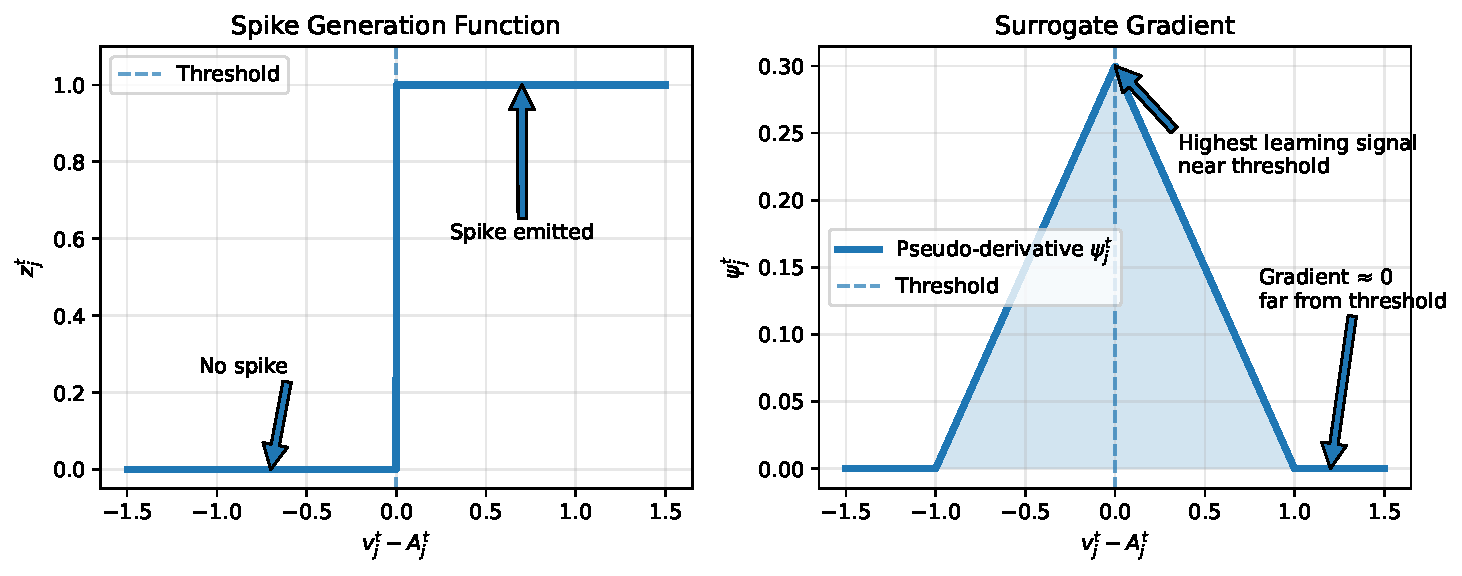
\includegraphics[width=\linewidth]{images/spiking_function_dynamics.pdf}
      \\{\scriptsize Membrane dynamics, spike and surrogate $\psi$.}
    \end{column}
  \end{columns}
  \note{$\psi$ returns later - it is the load-bearing ingredient of Contribution 2.}
\end{frame}

% ---- 3. E-prop = trace x signal -----------------------------
\begin{frame}{E-prop: a local trace $\times$ a learning signal}
  \citet*{} \textbf{E-prop}~\citep{eprop2020} factorizes the gradient into
  two pieces each neuron holds at any time:
  \[
    \frac{dE}{dW_{ji}}
      \;=\; \sum_t \underbrace{L_j^t}_{\text{learning signal}}\;
                   \cdot \underbrace{e_{ji}^t}_{\text{eligibility trace}}
  \]
  \begin{columns}[T]
      \begin{column}{0.45\textwidth}
    \begin{block}{Learning signal $L_j^t$: ``how much did my spike affect the loss?''}
      An approximation of $\frac{dE}{dz_j^t}$, routed top-down
      via feedback weights (one scalar per neuron, per time step).
    \end{block}
    \end{column}
    \begin{column}{0.45\textwidth}
    \begin{block}{Eligibility trace $e_{ji}^t$: ``how much did this synapse contribute to my spike?''}
      The derivative of neuron $j$'s spike w.r.t.\ weight $W_{ji}$,
      accumulated forward in time.
    \end{block}
    \end{column}
  \end{columns}
  \vfill
  \centering Sidesteps both BPTT's and RTRL's memory/compute cost.
  \note{Emphasise: this is the framework everything else is built on.}
\end{frame}

\begin{frame}{Why e-prop matters, beyond cost}
  Two properties worth noting relative to TBPTT:
  \vfill
  \begin{columns}[T]
    \begin{column}{0.48\textwidth}
      \begin{block}{Reuse, not recomputation}
        TBPTT recomputes a backward pass of cost $\mathcal{O}(k)$ for every
        timestep it updates at. E-prop's trace is a forward recursion: each
        step reuses the previous step's trace directly, there is no per-update
        backward pass cost to pay.
      \end{block}
    \end{column}
    \begin{column}{0.48\textwidth}
      \begin{block}{Stable at any depth}
        TBPTT's gradient is a product of Jacobians chained across the
        window, the usual vanishing/exploding problem, worsened by the recurrences. E-prop's trace is a single neuron's own local
        and stable recursion dependent on presynaptic activity, and the learning signal does not compound either.
      \end{block}
    \end{column}
  \end{columns}
\end{frame}
% (place immediately after the e-prop factorisation frame, in Background)
\begin{frame}{E-prop: ALIF detailed formulas}
  Neuron dynamics, pseudo-derivative, and the local trace:
  \begin{align*}
    v^t_j &= \alpha\, v^{t-1}_j + \textstyle\sum_i W_{ji} z^{t-1}_i
             - z^{t-1}_j v_{\mathrm{th}},
      & z^t_j &= H(v^t_j - A^t_j)\\
    \psi^t_j &= \tfrac{\gamma_{\mathrm{pd}}}{v_{\mathrm{th}}}
      \max\!\big(0,\,1 - |\tfrac{v^t_j - A^t_j}{v_{\mathrm{th}}}|\big)
      & e^t_{ji} &= \psi^t_j\big(\bar{z}^t_i - \beta\,\epsilon^{t-1}_{ji}\big)
  \end{align*}
  Gradient factorisation:
  \[
    \frac{\mathrm{d}E}{\mathrm{d}W_{ji}} = \sum_t L^t_j\, \bar{e}^{\,t}_{ji},
    \qquad L^t_j \approx \frac{\mathrm{d}E}{\mathrm{d}z^t_j}.
  \]
  For LIF ($\beta=0$): $e^t_{ji} = \psi^t_j\,\bar{z}^t_i$.
\end{frame}

% ---- 4. The weak point: feedback weights --------------------
\begin{frame}{E-prop: Structured feedback weights}
  Where does $L_j^t$ come from? The true $\frac{dE}{dz_j^t}$
  is intractable online as it requires knowing how neuron $j$'s spike
  propagates through future time steps. Random/Adaptive e-prop replaces it with
  currently arising output errors routed via feedback weights $B_{jk}$.
  \vfill
  This introduces two sources of bias:
  \begin{itemize}
    \item \textbf{Temporal:} indirect effects through future time steps
          are ignored.
    \item \textbf{Structural:} $B_{jk}$ is a linear projection, it is
          insufficient to represent even $\frac{\partial E}{\partial z_j^t}$
          for neurons beyond causal path length 1, where the true signal
          involves nonlinear dependencies.
  \end{itemize}
  \vfill
  Despite this, the authors report no task where e-prop fails where
  BPTT succeeds, the approximation is empirically robust.
  \vfill

\end{frame}

% ---- 5. RL briefly + TD error -------------------------------
\begin{frame}{Reinforcement learning, briefly}
  \begin{columns}[T]
    \begin{column}{0.45\textwidth}
      \begin{block}{The loop}
        An agent acts in an environment and receives a \textbf{reward};
        the goal is to maximize reward over time.
      \end{block}
      \begin{block}{Actor \& critic}
        A \textbf{critic} estimates the value $V$ (expected future reward);
        an \textbf{actor} chooses actions to push it up.
      \end{block}
    \end{column}
    \begin{column}{0.45\textwidth}
      \begin{alertblock}{TD error: the reward signal}
        \[
          \delta_t \;=\; r_t + \gamma V_{t+1} - V_t
        \]
        Positive $\delta$ = ``better than expected.''
        Negative $\delta$ = ``worse than expected.'' \\
        This single scalar becomes the learning signal.
        
        The hyperparameter $\gamma$ sets how far the critic looks ahead.
      \end{alertblock}
    \end{column}
  \end{columns}
  \note{$\delta$ is the one number that will be broadcast to every neuron.}
\end{frame}



\begin{frame}{Reward-based e-prop}
  The TD error plugs into the e-prop update as a global modulator:
  \[
    \Delta W_{ji} = -\eta \sum_t \delta_t\,
      \mathcal{F}_{\gamma}\!\left(L_j^t\, \bar{e}^{\,t}_{ji}\right)
  \]
  with the neuron-specific learning signal decomposed as:
  \[
    L_j^t = -c_V B_j^V + \sum_k B_{kj}^\pi \,
      \nabla_{\theta} \log \pi_k^t
    \;;\quad
    \nabla_{\theta} \log \pi_k^t = \pi_k^t - \mathbf{1}_{a^t=k} \ (Softmax)
  \]
  \begin{columns}[T]
    \begin{column}{0.31\textwidth}
      \begin{block}{$\delta_t$: prediction error}
        Global TD error, broadcast identically to every synapse.
      \end{block}
    \end{column}
    \begin{column}{0.31\textwidth}
      \begin{block}{$L_j^t$: policy \& value feedback}
        Neuron-specific combination of value and policy gradients,
        routed via feedback weights $B^V_j$, $B^\pi_{kj}$.
      \end{block}
    \end{column}
    \begin{column}{0.31\textwidth}
      \begin{block}{$\bar{e}^{\,t}_{ji}$: synaptic responsibility}
        Local eligibility trace: which synapses matter most and how.
      \end{block}
    \end{column}
  \end{columns}
  \note{This is the baseline the two contributions improve upon.}
\end{frame}
% ============================================================
%  CHUNK 3 / 6 : Contributions
% ============================================================
\section{Contributions}

% ---- 1. Two contributions overview --------------------------
\begin{frame}{Two contributions}
  This thesis asks whether recurrent spiking networks can learn online using
  only local computation and a globally broadcast signal, addressed through
  two contributions.
  \begin{columns}[T]
    \begin{column}{0.45\textwidth}
      \begin{block}{1 - A continuously-running online RL agent}
        An excitatory-inhibitory recurrent SRNN trained \textbf{online} with
        e-prop, \textbf{no episodic resets}, on a GPU-accelerated event-based
        simulator~\citep{Yavuz2016GeNN}. As part of this, we integrate
        TD($\lambda$) into the e-prop update and \textbf{decouple} the
        discount $\gamma$ from the credit-trace decay $\lambda$.
      \end{block}
    \end{column}
    \begin{column}{0.45\textwidth}
      \begin{block}{2 - Distributed e-prop}
        A new family of rules that \textbf{eliminates the structured feedback
        weights}, every neuron receives the same single broadcast scalar and
        relies entirely on its own local activity to update its incoming
        connections.
      \end{block}
    \end{column}
  \end{columns}
\end{frame}

% (place immediately after "Two contributions", in Contributions)
\begin{frame}{Network architecture}
  \begin{columns}[T]
    \begin{column}{0.3\textwidth}
      \begin{itemize}\small
        \item Excitatory–inhibitory recurrent core (weakened Dale's law)
              \citep{Song2016DaleEI,Cornford2021DaleANN}.
        \item Per-head EI field layers between core and outputs, these increase the
              \emph{causal path length} between the input and the output.
        \item Toroidal Gaussian connectivity
              \citep{Spreizer2019Toroidal}.
      \end{itemize}
    \end{column}
    \begin{column}{0.7\textwidth}
      \centering
      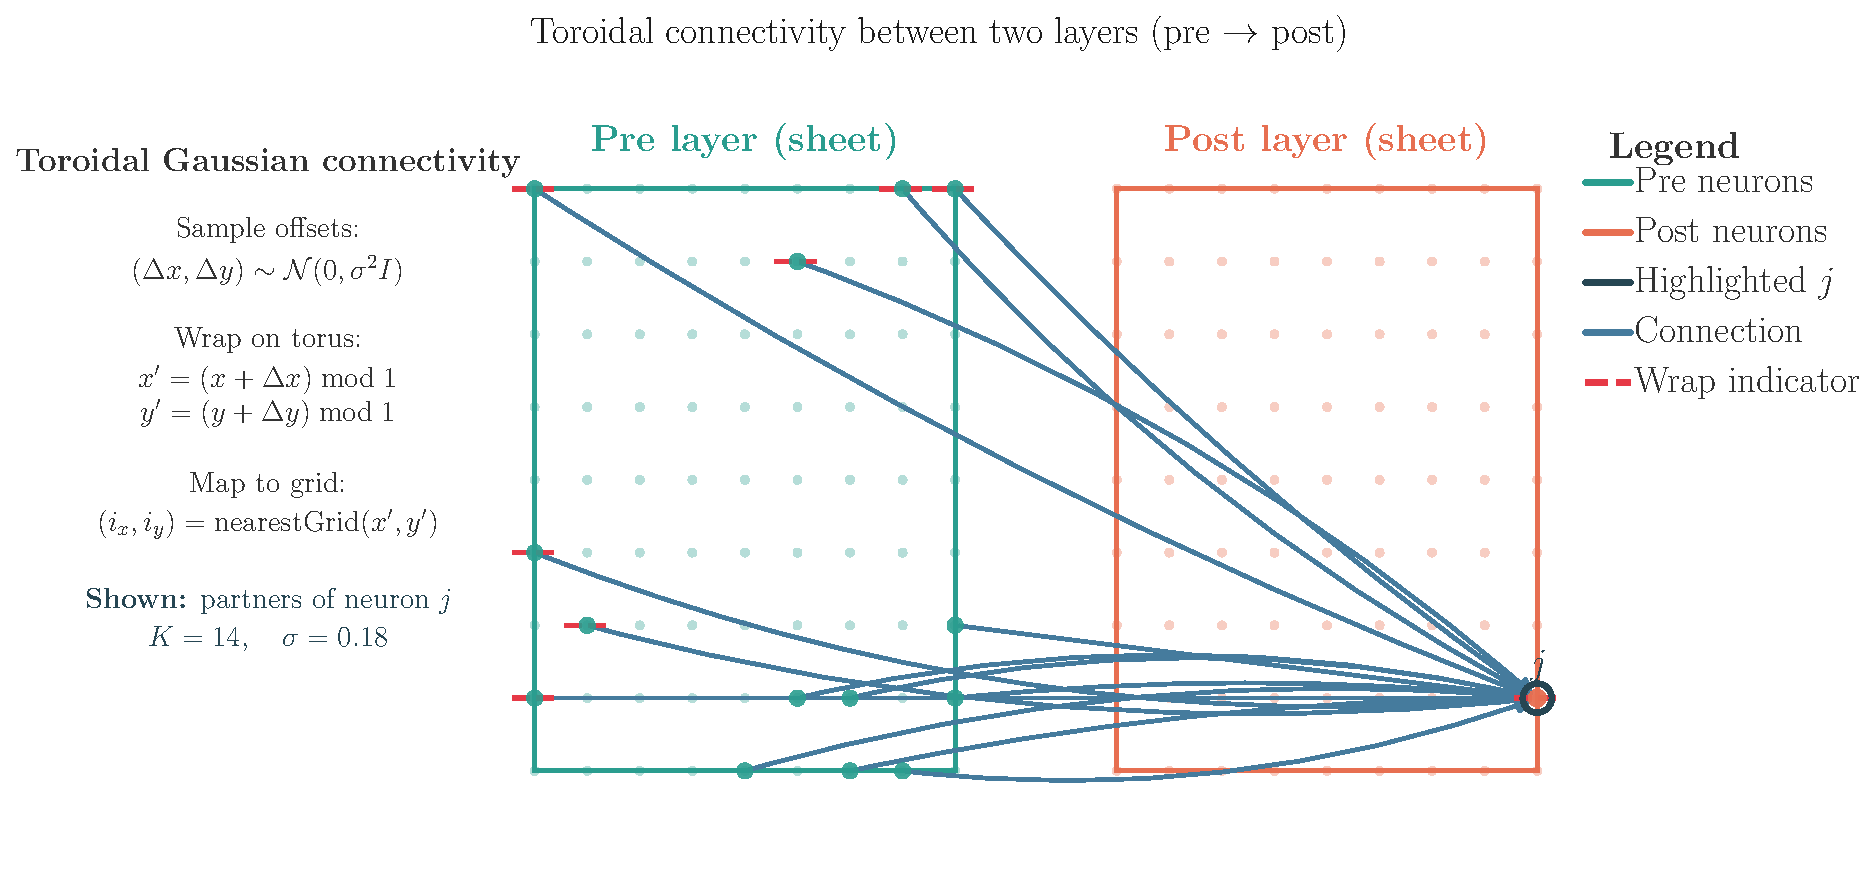
\includegraphics[width=\linewidth]{images/toroidal_connectivity_two_layers.pdf}
    \end{column}
  \end{columns}
\end{frame}

% ---- 2. TD(lambda) inside e-prop ----------------------------
\begin{frame}{TD($\lambda$) with e-prop}
  The online reward-based e-prop update filters the local signal with the
  discount $\gamma$:
  $$
    \Delta W_{ji} = -\eta \sum_t \delta_t\,
      \mathcal{F}_{\gamma\lambda}\!\left(L_j^t\, \bar{e}^{\,t}_{ji}\right)
  $$
  $$
    p^{\,t}_{ji} = \gamma\lambda\, p^{\,t-1}_{ji} + L_j^t\, \bar{e}^{\,t}_{ji}
    \;\equiv\;
    \mathcal{F}_{\gamma\lambda}\!\left(L_j^t\, \bar{e}^{\,t}_{ji}\right)
  $$
  
  Relaxing the credit-trace decay from $\gamma$ to $\gamma\lambda$ recovers the
  backward view of TD($\lambda$)~\citep{SuttonBarto2018}: $\lambda$ spreads
  credit for an action back over a tunable horizon.
  \vfill
  \begin{alertblock}{The catch}
    Since $\gamma\lambda \le \gamma$, a \emph{small} $\gamma$ caps the credit
    horizon no matter how large $\lambda$ is, the credit trace collapses to a small number of actions.
  \end{alertblock}
\end{frame}

% ---- 3. Decoupling gamma and lambda -------------------------
\begin{frame}{Decoupling $\gamma$ and $\lambda$}
  One parameter, two conflicting jobs: \alert{stable critic} wants $\gamma$
  \emph{small}; \alert{long action credit} wants the horizon \emph{long}.
  We separate them.
  \begin{columns}[T]
    \begin{column}{0.55\textwidth}
      \vspace{0.5em}
      \textbf{Input / hidden weights} $\lambda$ alone sets the horizon:
      \[ h^{\,t}_{ji} = \lambda\, h^{\,t-1}_{ji} + L_j^t\, \bar{e}^{\,t}_{ji}
         \;\equiv\; \mathcal{F}_{\lambda}\!\left(L_j^t\, \bar{e}^{\,t}_{ji}\right) \]
      \textbf{Actor output weights} Actors use the same $\lambda$:
      \[ p^{\,t}_{kj} = \lambda\, p^{\,t-1}_{kj} +  \nabla_{\theta} \log \pi_k^t\, \bar{z}^{\,t}_{j}
         \;\equiv\; \mathcal{F}_{\lambda}\!\left( \nabla_{\theta} \log \pi_k^t\, \bar{z}^{\,t}_{kj}\right) \]
      \textbf{Critic output weights} keeps $\gamma$:
      \[ \nu^{\,t}_{kj} = \gamma\, \nu^{\,t-1}_{kj} + \bar{z}^{\,t}_{j}
         \;\equiv\; \mathcal{F}_{\gamma}\!\left(\bar{z}^{\,t}_{i}\right) \]
      $\Rightarrow$ long-range credit \emph{without} destabilizing the critic.
    \end{column}
    \begin{column}{0.45\textwidth}
      \centering
      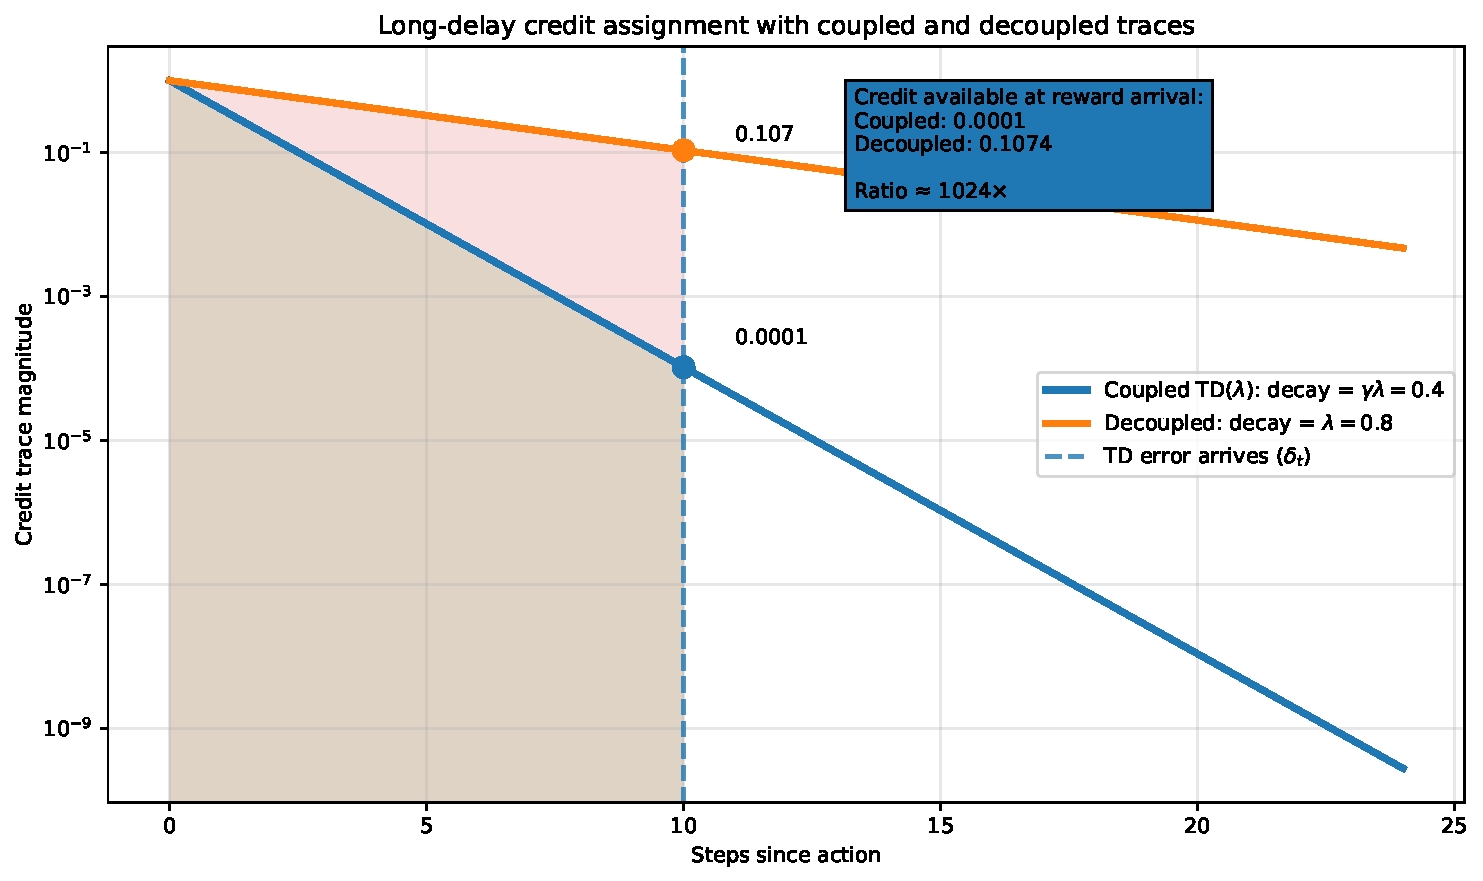
\includegraphics[width=\linewidth]{images/credit_trace_comparison.pdf}\\
      {\scriptsize Decoupled trace (decay $\lambda$) keeps credit alive
       far longer than the coupled $\gamma\lambda$ trace.}
    \end{column}
  \end{columns}
\end{frame}

% (place immediately after "Decoupling γ and λ")
\begin{frame}{Multi-step actions and interpretation of $\lambda$, $\gamma$}
  Each action is held for $\Delta$ neural integration steps. To keep
  $\gamma,\lambda$ meaningful at the \emph{behavioural} (per-action) level
  regardless of $\Delta$, we take the per-step decay as the $\Delta$-th root:
  \[
    \gamma_{\text{step}} = \gamma^{1/\Delta}, \qquad
    \lambda_{\text{step}} = \lambda^{1/\Delta}
  \]
  so that $\Delta$ compounding steps reproduce exactly the chosen per-action
  decay, $\Delta$ drops out of the effective horizon. Decoupled, the two
  constants then read independently:
  \begin{itemize}\small
    \item $\gamma$ - critic's value horizon / bootstrapping; kept small for a
          stable spike-based critic.
    \item $\lambda$ - pure credit window of order $1/(1-\lambda)$ steps; can sit
          near $1$ even when $\gamma$ is small.
  \end{itemize}
  Self-limiting: once the critic predicts rewards well, the extra terms a larger
  $\lambda$ contributes vanish.
\end{frame}

% ---- 4. Distributed e-prop: neurons as stochastic actors ----
\begin{frame}{Distributed E-prop}
  Remove the feedback weights altogether: treat every neuron as an
  \textbf{independent stochastic actor}, with the update
  \[
    \Delta W_{ji} \;\propto\;
      \delta_t \cdot \frac{(1-\alpha^2)\,\xi_j^t}{\sigma_j^2} \cdot e^{\,t}_{ji}
  \]
  Each neuron perturbs its own membrane dynamics and correlates that local
  noise with the single global TD error $\delta_t$:
  \[ v_j^t \sim \mathcal{N}(\mu_j^t,\, \sigma_j^2),
     \qquad \varepsilon_j^t = v_j^t - \mu_j^t,
     \qquad \xi_j^t = \alpha\,\xi_j^{t-1} + \varepsilon_j^t \]
  Grounded in node/weight-perturbation learning~\citep{Cauwenberghs1992}
  and its established link to policy
  gradients~\citep{Williams1992REINFORCE,fiete2006gradient}.
  \vfill
  \centering\small
  What makes this \emph{e-prop}: the raw estimate is weighted by
  $\psi_j^t$, so it only counts perturbations near threshold, and
  $\psi_j^t\,\epsilon^{\,t,v}_{ji}$ is precisely the e-prop trace
  $e^{\,t}_{ji}$ (LIF case; for ALIF, we extend this to keep using the
  e-trace as a natural but heuristic choice).
\end{frame}

% ---- 5. One broadcast scalar - the update rule --------------
\begin{frame}{Every neuron, the same broadcast scalar}
  No structured routing: one identical number $\delta_t$ reaches every neuron,
  combined with information it already holds.
  
    The filtered perturbation
  trace $\xi_j^t = \alpha\,\xi_j^{t-1} + \varepsilon_j^t$ is the membrane shift
  attributable to noise alone, beyond what deterministic dynamics would
  have produced:
  \[
    \Delta W_{ji} \;\propto\;
      \delta_t\;
      \mathcal{F}_{\lambda}\!\left(
        \underbrace{\tfrac{(1-\alpha^2)\,\xi_j^t}{\sigma_j^2}}_{\text{perturbation footprint}}
        \;\cdot\;
        \underbrace{e^{\,t}_{ji}}_{\text{synapse sensitivity}}
      \right)
  \]
  \begin{center}\small
    \alert{$\delta_t$} = was it good? \quad
    \alert{$\xi_j^t$} = which way did noise push me? \quad
    \alert{$e^{\,t}_{ji}$} = was this synapse responsible?
  \end{center}
  \vfill
  \centering\footnotesize
  
  $(1-\alpha^2)$ corrects $\xi_j^t$ back to the perturbation's own variance
  (filtering inflates it)
  
  $1/\sigma_j^2$ falls out of the Gaussian policy's score function.
  \vfill
\end{frame}

% ---- 6. psi-gating: the essential ingredient ----------------
\begin{frame}{The essential ingredient: gating by $\psi$}
  The actor's "action'' is the perturbation \(\varepsilon_j^t\) on the
  \textbf{membrane potential}, not the spike itself, so the policy-gradient
  derivation never touches $z_j^t$, and $\psi$ does not appear naturally.
  \vfill
  Yet a membrane nudge only matters when it's near threshold, the only
  moment it can flip whether the neuron spikes. We gate the update by the
  pseudo-derivative anyway, recovering the e-prop eligibility trace
  $e^{\,t}_{ji} = \psi_j^t\,\epsilon^{\,t,v}_{ji}$~\citep{eprop2020}.
  \vfill
  \begin{columns}[T]
    \begin{column}{0.45\textwidth}
      \begin{block}{With $\psi$-gating}
        Credit lands where it counts. Stable dynamics, effective learning.
      \end{block}
    \end{column}
    \begin{column}{0.45\textwidth}
      \begin{alertblock}{Without it (ablation)}
        Performance collapses below every variant; membrane voltage seen to diverge
        without bound.
      \end{alertblock}
    \end{column}
  \end{columns}
  \vfill
  \centering\small
  The perturbation derivation never asked for $\psi$, but it is
  \textbf{load-bearing}.
\end{frame}

\begin{frame}{Backward routing of local gradients}
  \textbf{independent stochastic actor}.
  \centering
  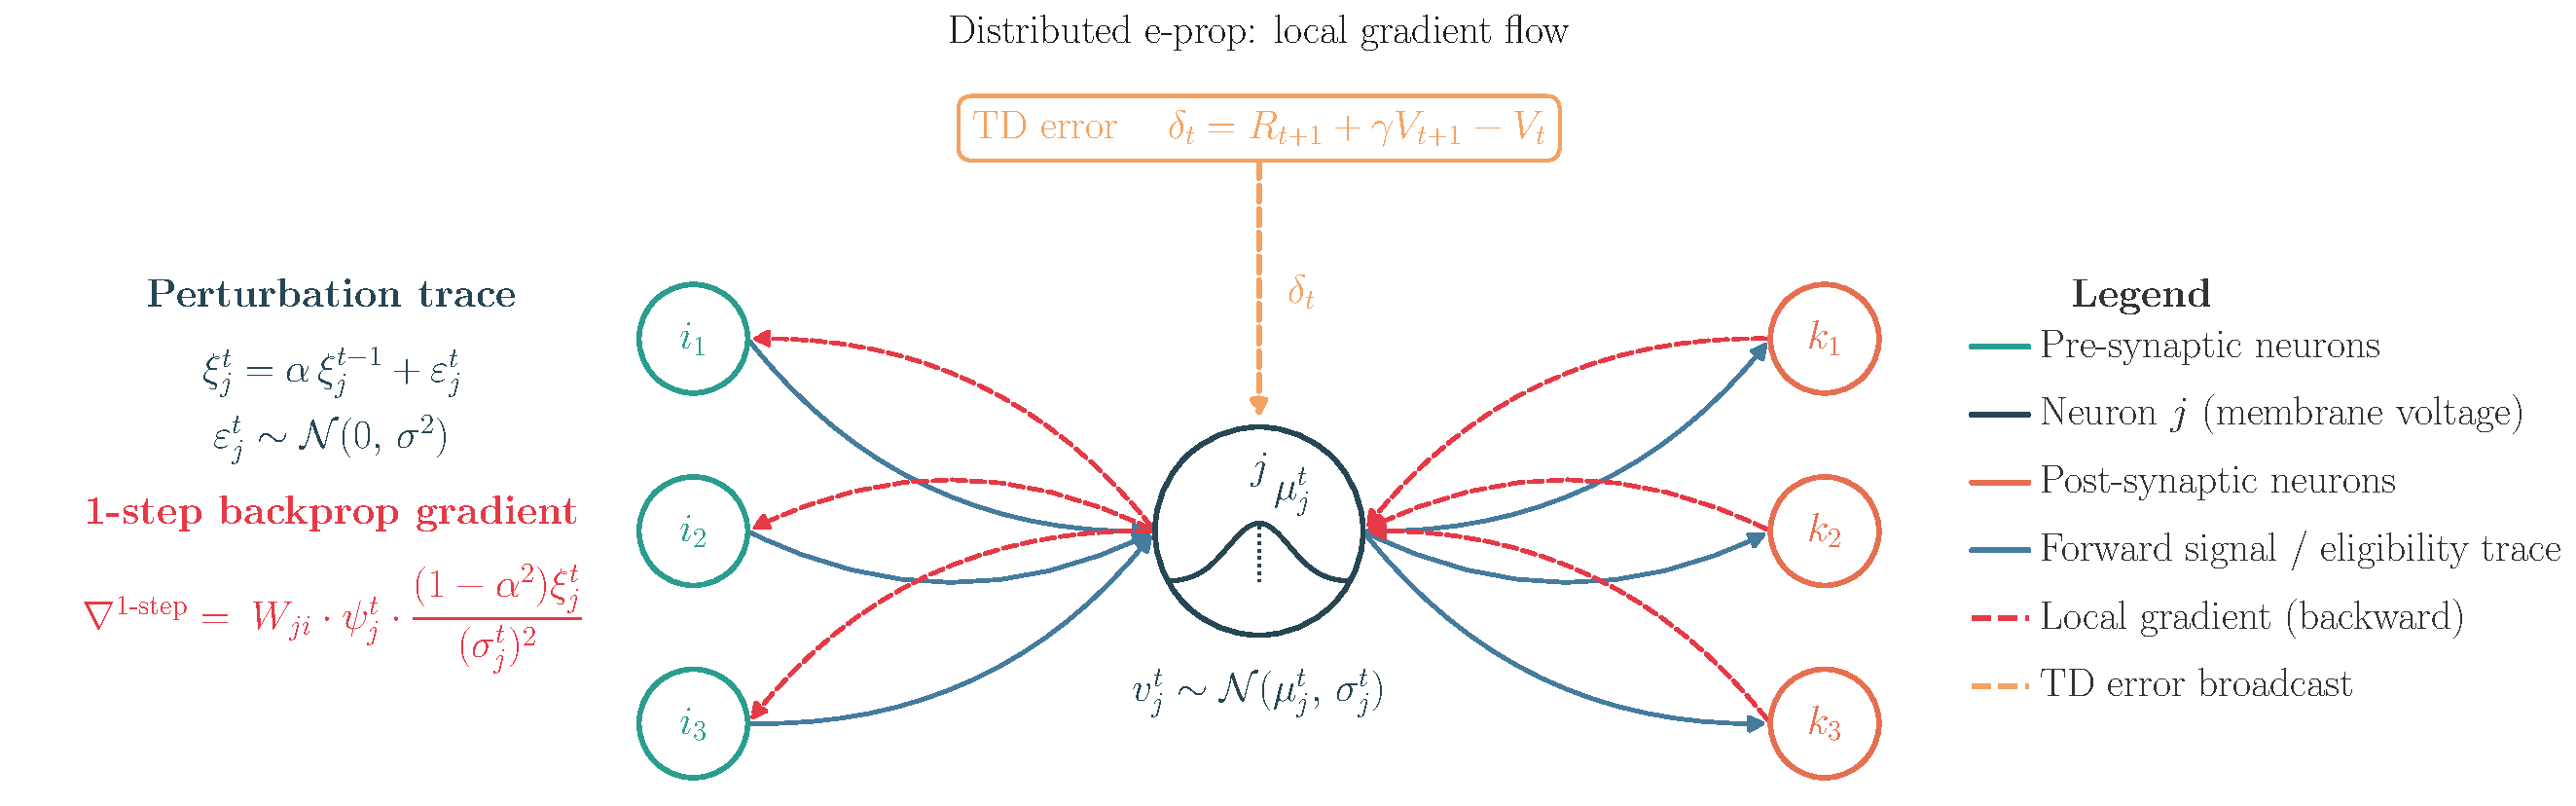
\includegraphics[width=\linewidth]{images/distributed_eprop_diagram.pdf}
\end{frame}

% ============================================================
%  CHUNK 4 / 6 : Experiments & Evaluation
% ============================================================
\section{Experiments \& Evaluation}

% ---- 1. Three tasks -----------------------------------------
\begin{frame}{Three tasks}
  Each probes a different facet of online credit assignment.
  \vfill
  \begin{columns}[T]
    \begin{column}{0.31\textwidth}
      \begin{block}{Snake $5\times5$}
        \begin{figure}
            \centering
            
\includegraphics[width=0.25\linewidth]{snake.png}
        \end{figure}
        \textbf{Reward credit assignment.} Eat food, grow longer; reward is
        frequent and fairly direct. Previous actions matter a lot.
      \end{block}
    \end{column}
    \begin{column}{0.31\textwidth}
      \begin{block}{Pac-Man}
        \begin{figure}
            \centering
            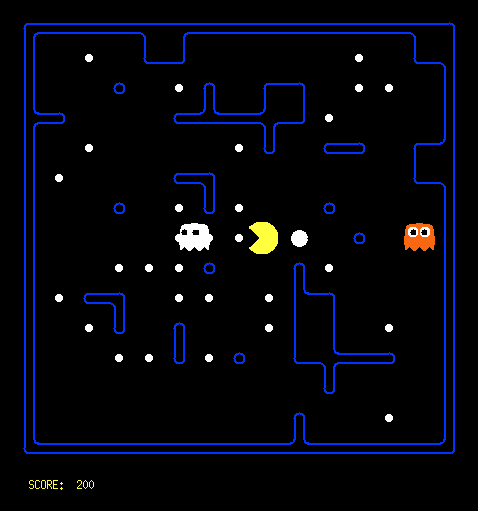
\includegraphics[width=0.25\linewidth]{pac-man.png}
        \end{figure}
        \textbf{Memory and partial observability.} Randomized layouts demand
        anticipatory navigation from limited views.
      \end{block}
    \end{column}
    \begin{column}{0.31\textwidth}
      \begin{block}{Connect Four}
        \begin{figure}
            \centering
            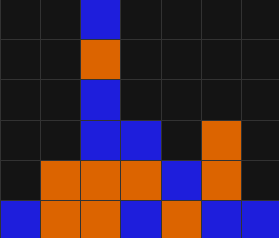
\includegraphics[width=0.25\linewidth]{connect-4.png}
        \end{figure}
        \textbf{Sparse reward.} A single reward at the end of the game, the
        hardest credit problem.
      \end{block}
    \end{column}
  \end{columns}
  \vfill
  \centering\small Pac-Man environment adapted from \citet{denero2010pacman}.
\end{frame}

% ---- 2. What we compare and how we measure ------------------
\begin{frame}{What we compare, and how we measure}
  \begin{columns}[T]
    \begin{column}{0.45\textwidth}
      \begin{block}{The comparison}
        \deprop{} (this thesis) vs. \aeprop{} with adaptively learned feedback
        weights. PPO~\citep{schulman2017ppo} serves \emph{only} as an
 idealized gradient-based ceiling.
      \end{block}
    \end{column}
    \begin{column}{0.45\textwidth}
      \begin{block}{The measure}
        In a continuing, no-reset setting there is no episode to total up, so
        the \textbf{reward rate} is the natural measure of performance.
      \end{block}
    \end{column}
  \end{columns}
  \vfill
  \begin{center}
    Colour key for every plot:\quad
    {\color{accent2}\rule{1.2em}{0.5em}}~\aeprop\quad
    {\color{accent3}\rule{1.2em}{0.5em}}~\deprop
  \end{center}
\end{frame}

% ---- 3. PPO ceiling and the metric ---------------------------
\begin{frame}{PPO ceiling \& reward rate}
  \begin{columns}[T]
    \begin{column}{0.45\textwidth}
      With a large $\gamma=0.99$, the \textbf{episodic} and \textbf{continuing}
      objectives settle at visibly different operating points:
      \begin{itemize}\small
        \item Episodic: episode reward $\approx 22$, but reward rate
              $\approx 0.18$.
        \item Continuing: episode reward $\approx 8$, yet reward rate
              $\approx 0.24$.
      \end{itemize}
      The spiking agents optimize the continuing stream, so reward rate, not
      episodic return, is more aligned with the target.
    \end{column}
    \begin{column}{0.55\textwidth}
      \centering
        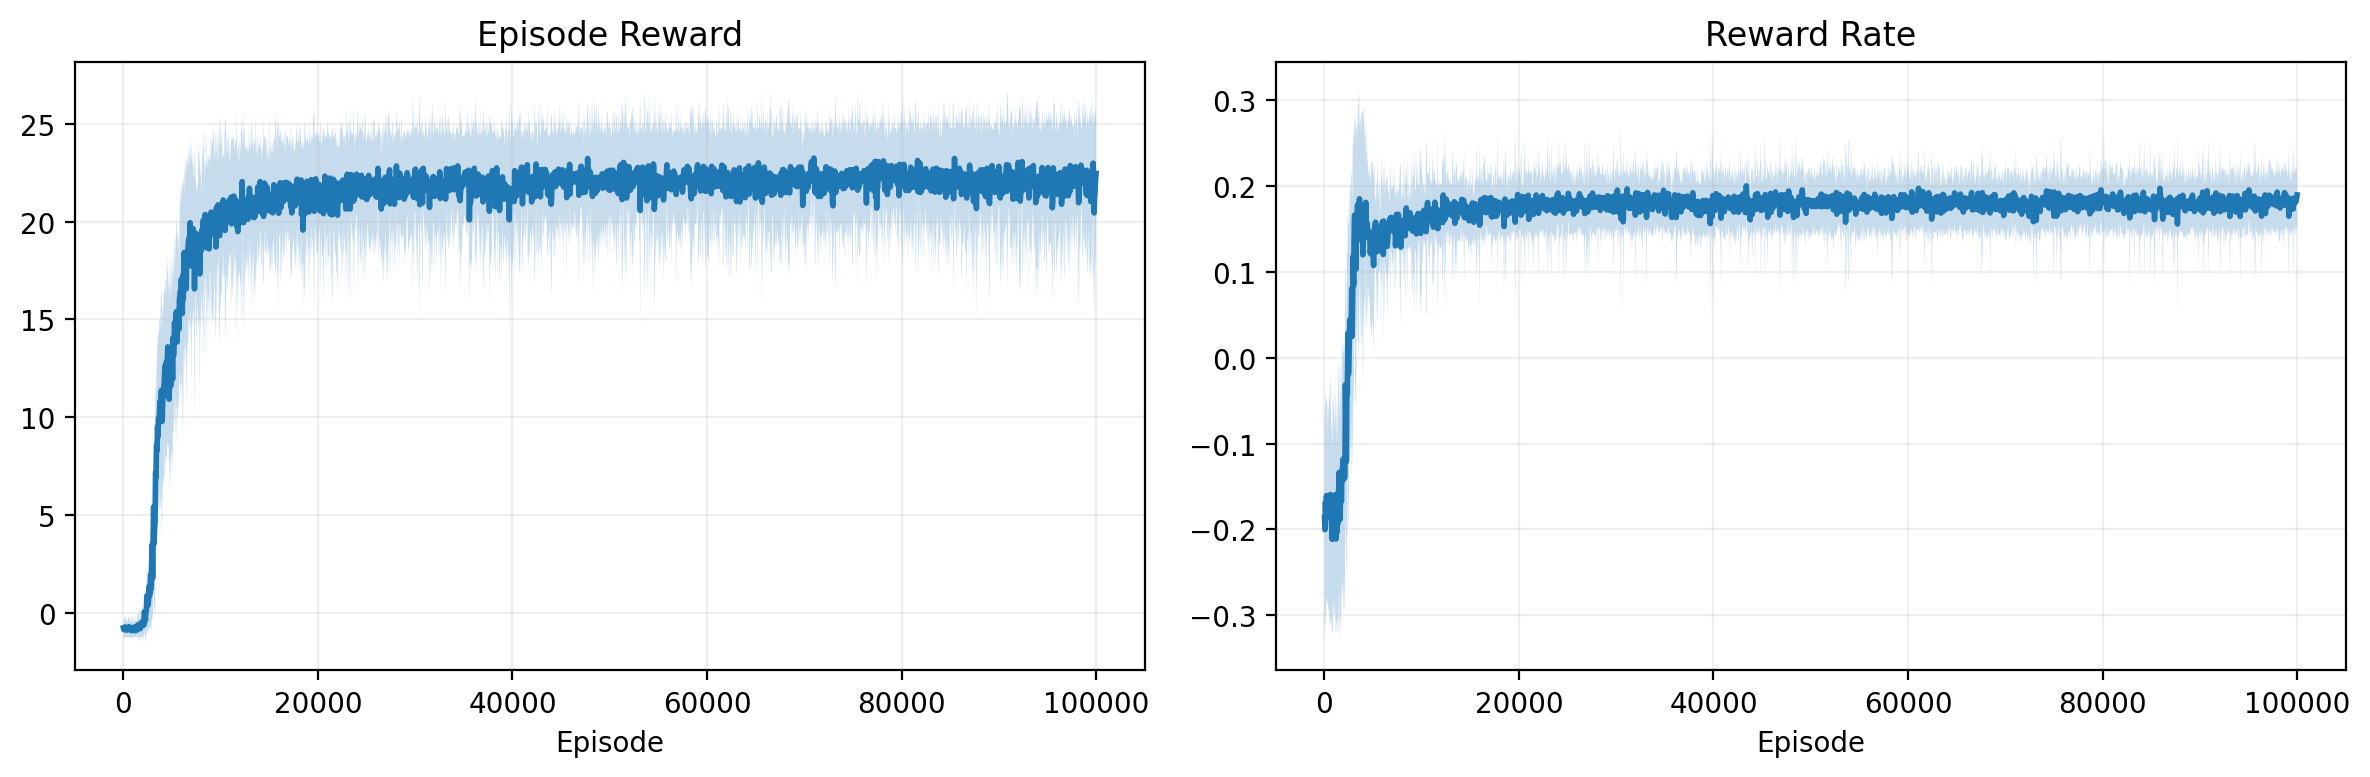
\includegraphics[width=\linewidth]{images/EpisodicObjectivePPO.png}
        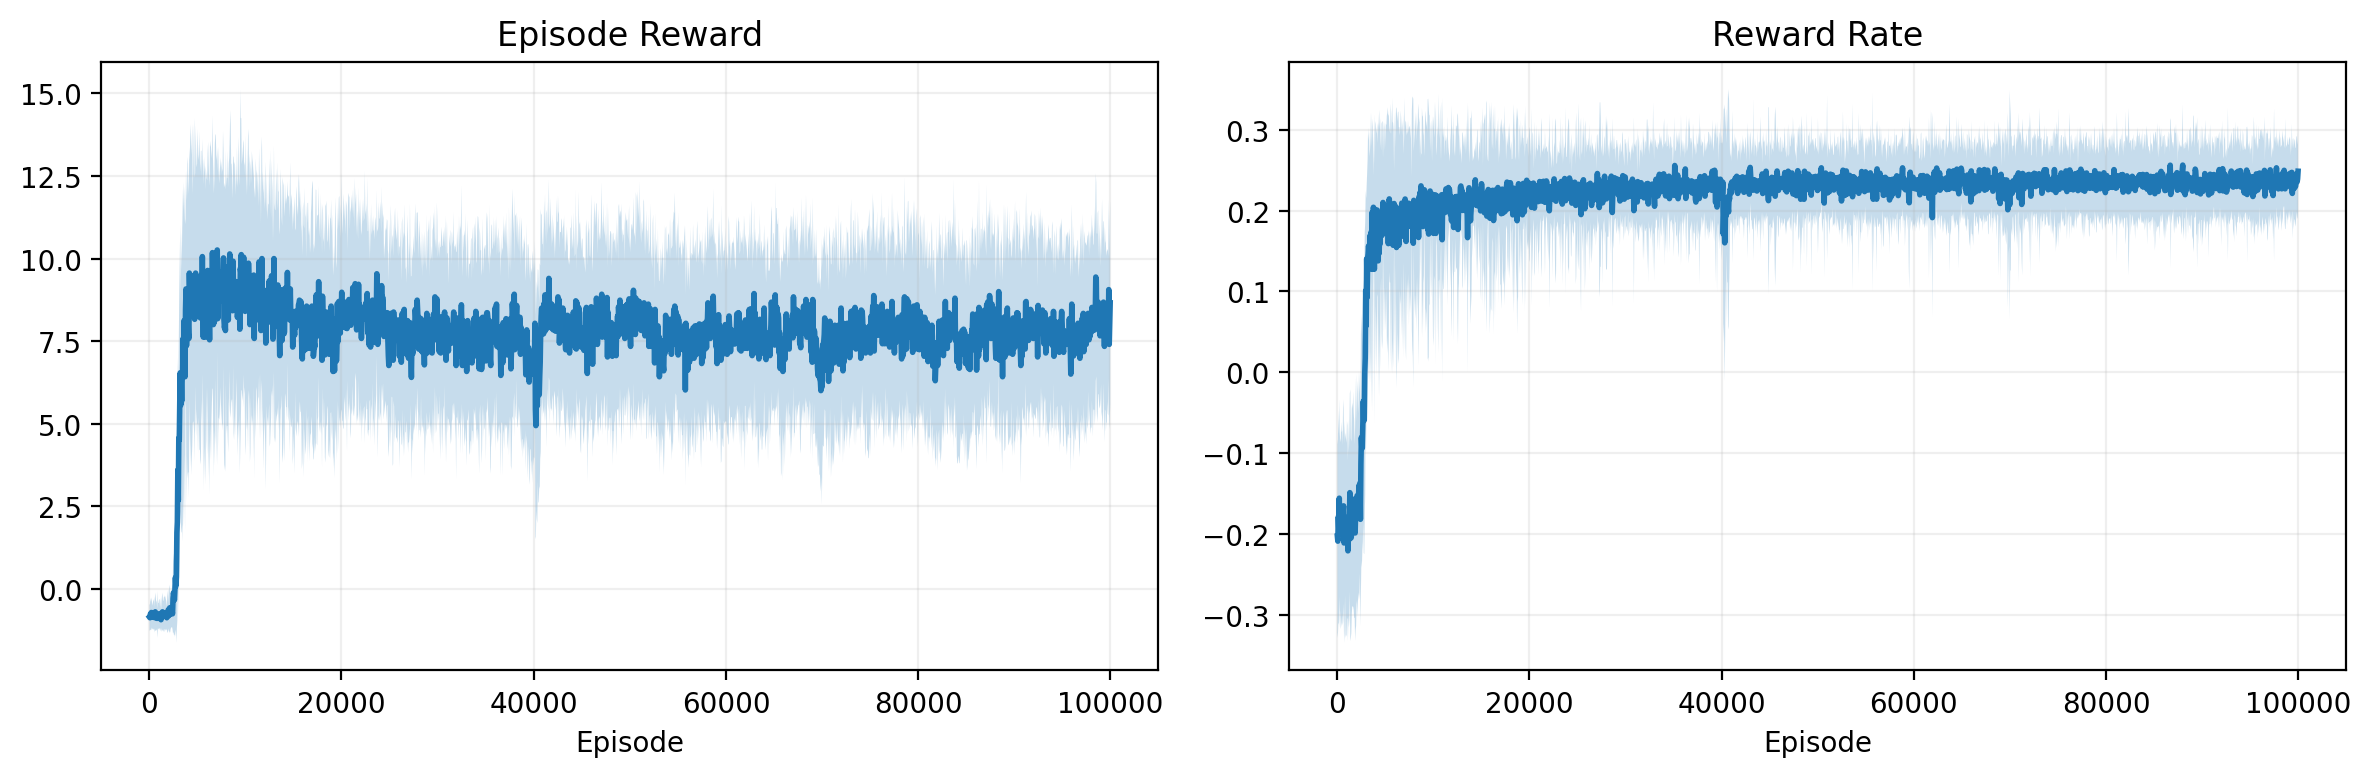
\includegraphics[width=\linewidth]{images/ContinuousObjectivePPO.png}
    \end{column}
  \end{columns}
\end{frame}

\begin{frame}{PPO at $\gamma=0.5$}
      At $\gamma=0.99$ the value horizon ($\sim$100 steps) spans most of an
      episode, so the two objectives pull apart. At $\gamma=0.5$, the same
      $\gamma,\lambda$ used by the spiking rules, the horizon shrinks to
      $\sim$2 steps: too short to reach either extreme, so episodic and
      continuing \textbf{coincide}: 
      
      episode reward $\approx 13$, reward rate $\approx 0.21$.
      \vfill
      \small Crucially, this lands almost exactly where \emph{symmetric}
      e-prop does.   The spiking rules aren't
      limited by their credit assignment; they're limited by $\gamma$ itself.
  \begin{columns}[T]
    \begin{column}{0.75\textwidth}
      \centering
      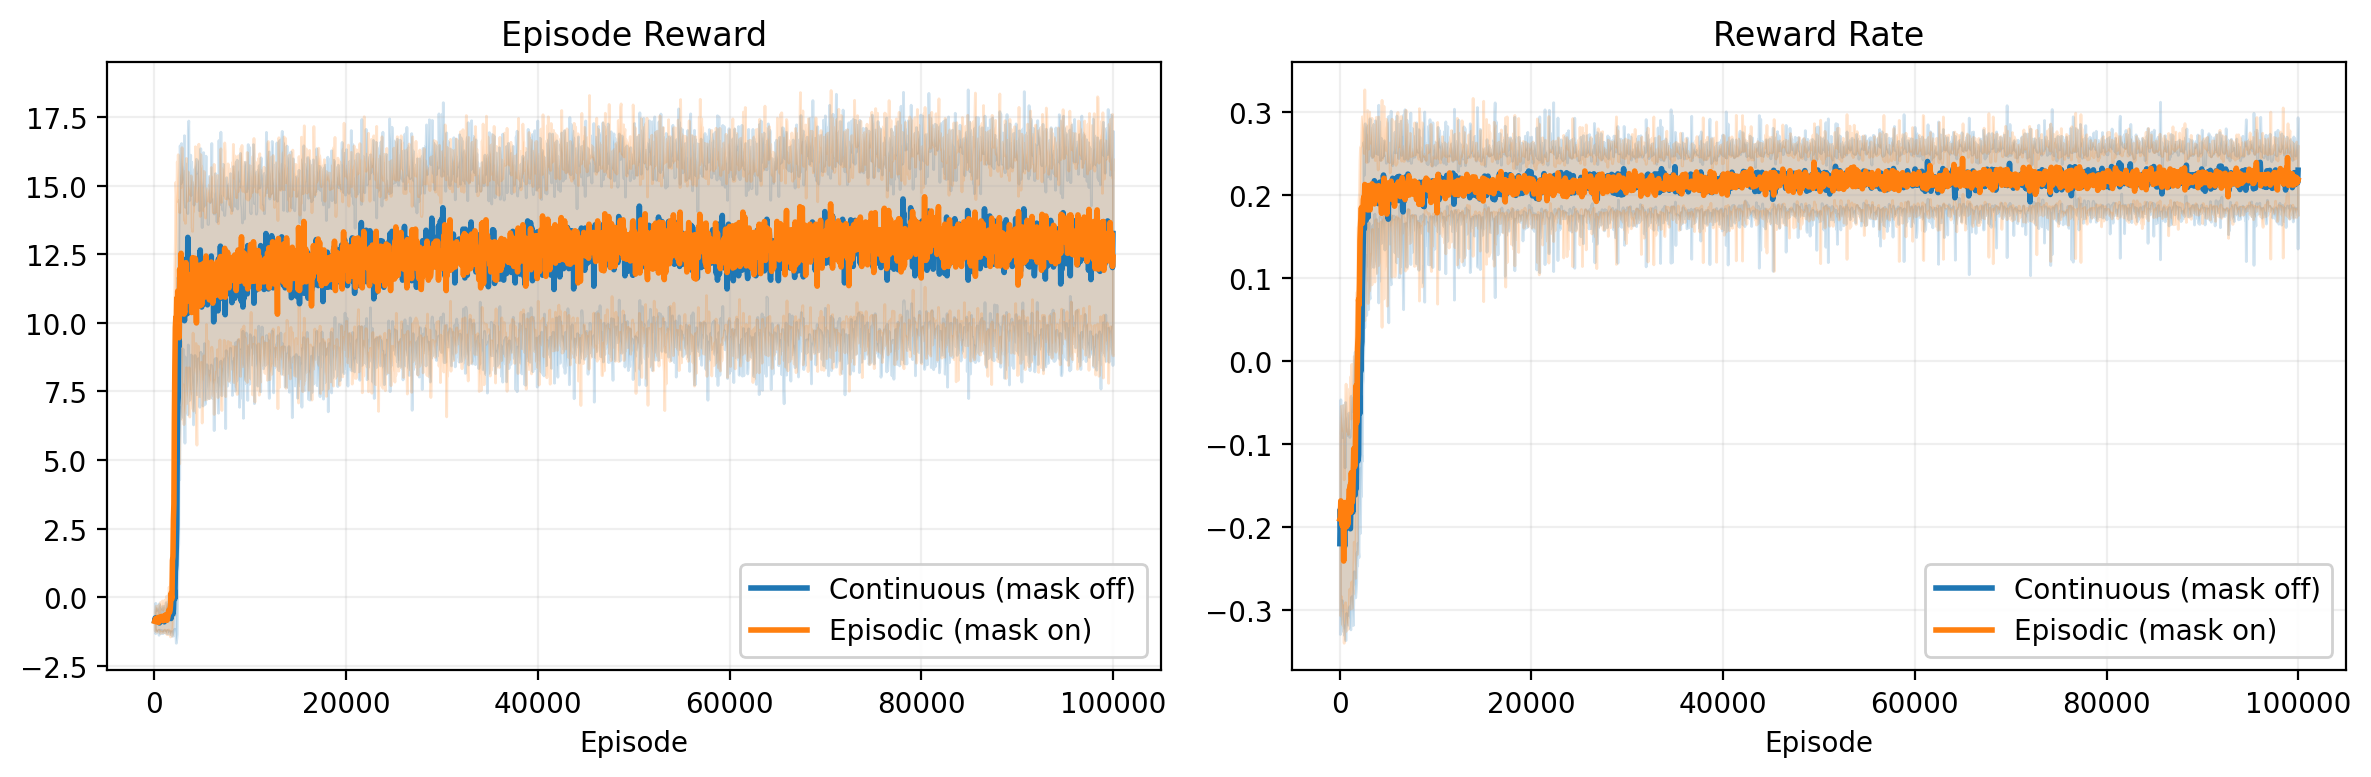
\includegraphics[width=\linewidth]{images/PPOComparison.png}
    \end{column}
  \end{columns}
\end{frame}

\begin{frame}{Symmetric e-prop performance and failure case}
  \begin{columns}[T]
    \begin{column}{0.48\textwidth}
      \emph{Symmetric} e-prop is the single strongest configuration on flat
      Snake $5\times5$.
      \vfill
      But insert per-head field layers and it \textbf{collapses entirely}: its
      feedback is tied to the forward output weights, so any neuron beyond
      causal path length $1$ receives \emph{no} signal.
      \vfill
      \begin{alertblock}{Why it matters}
        An outright failure mode, not gradual decay - this is what motivates
        both adaptive and distributed e-prop.
      \end{alertblock}
    \end{column}
    \begin{column}{0.52\textwidth}
      \centering
      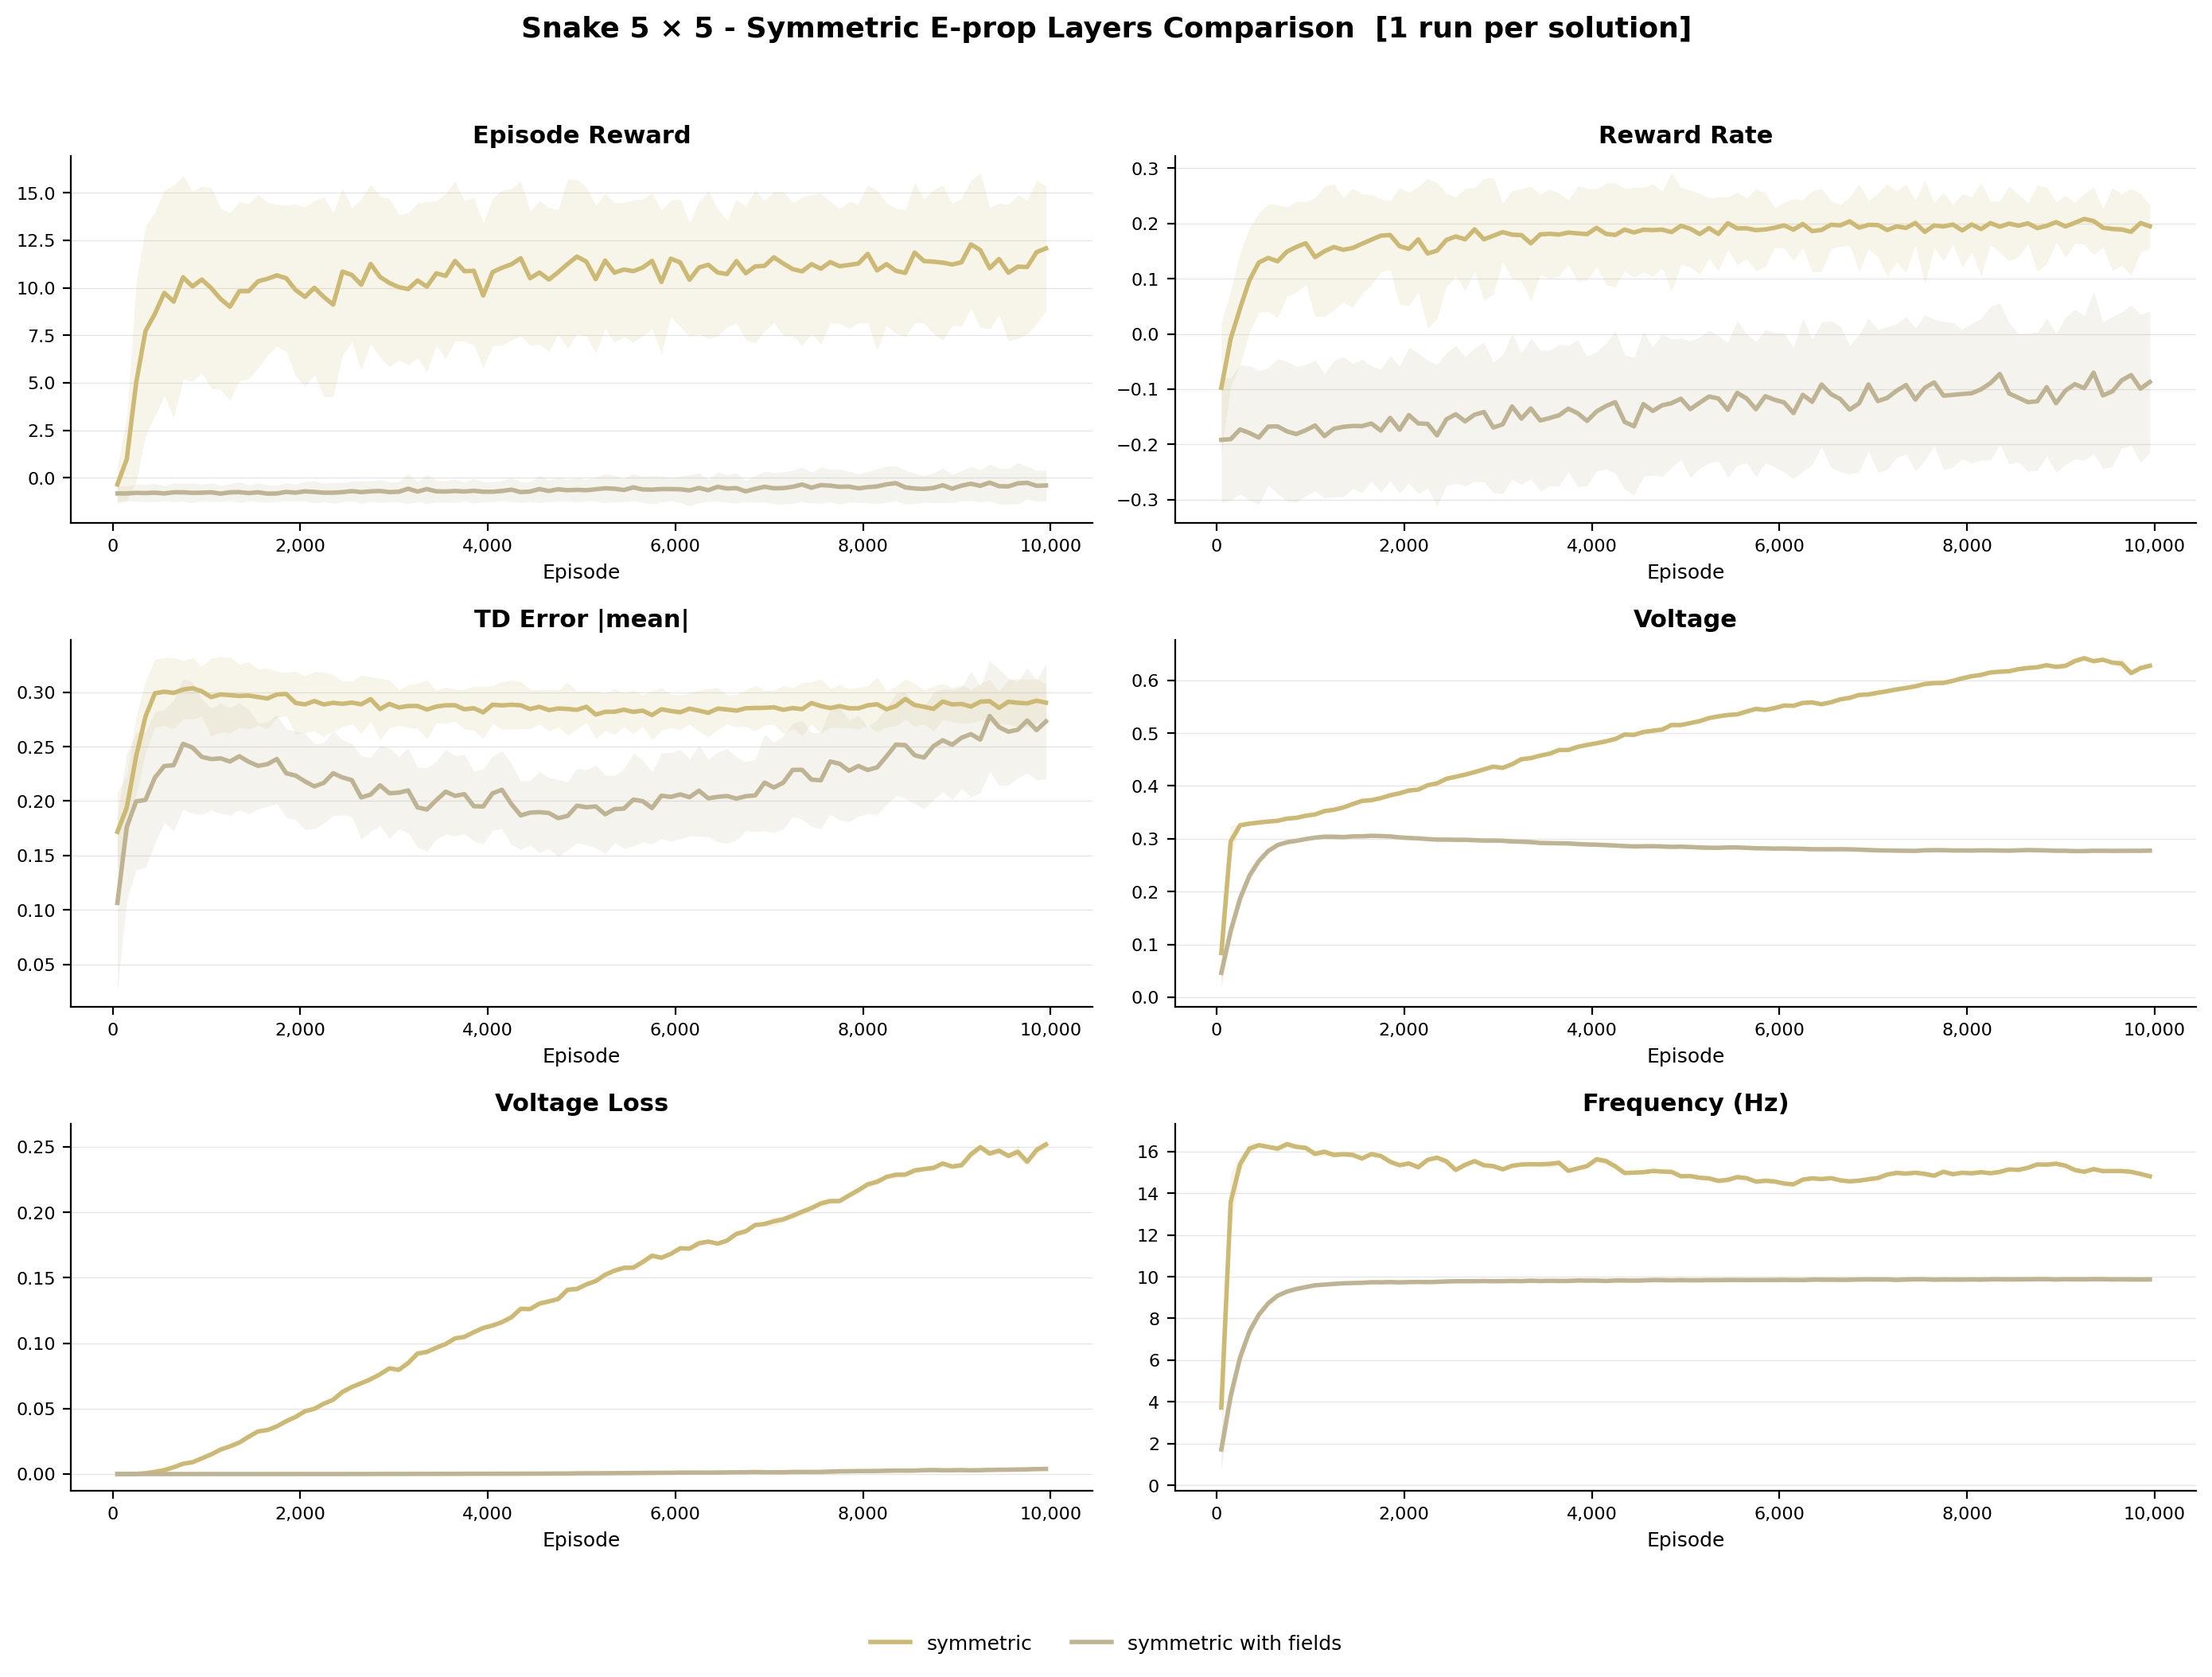
\includegraphics[width=\linewidth]{images/SnakeSymmetric.png}
    \end{column}
  \end{columns}
\end{frame}

% ---- 4. Snake result: competitive ----------------------------
\begin{frame}{Performance comparison on Snake $5\times5$}
  \begin{columns}[T]
    \begin{column}{0.4\textwidth}
     \begin{itemize}
         \item The neuron perturbation variants clearly underperform the weight perturbation variants.
         \item Independent noise per synapse hurt learning, the best variant found use the weight variant with noise at the post-synaptic neuron.
         \item Psi is essential, one of the wining variants drops to the worst performer by omiting Psi.
         \item Baseline tells us that training the recurrent structure is essential.
          
      
     \end{itemize}
    \end{column}
    \begin{column}{0.6\textwidth}
      \centering
      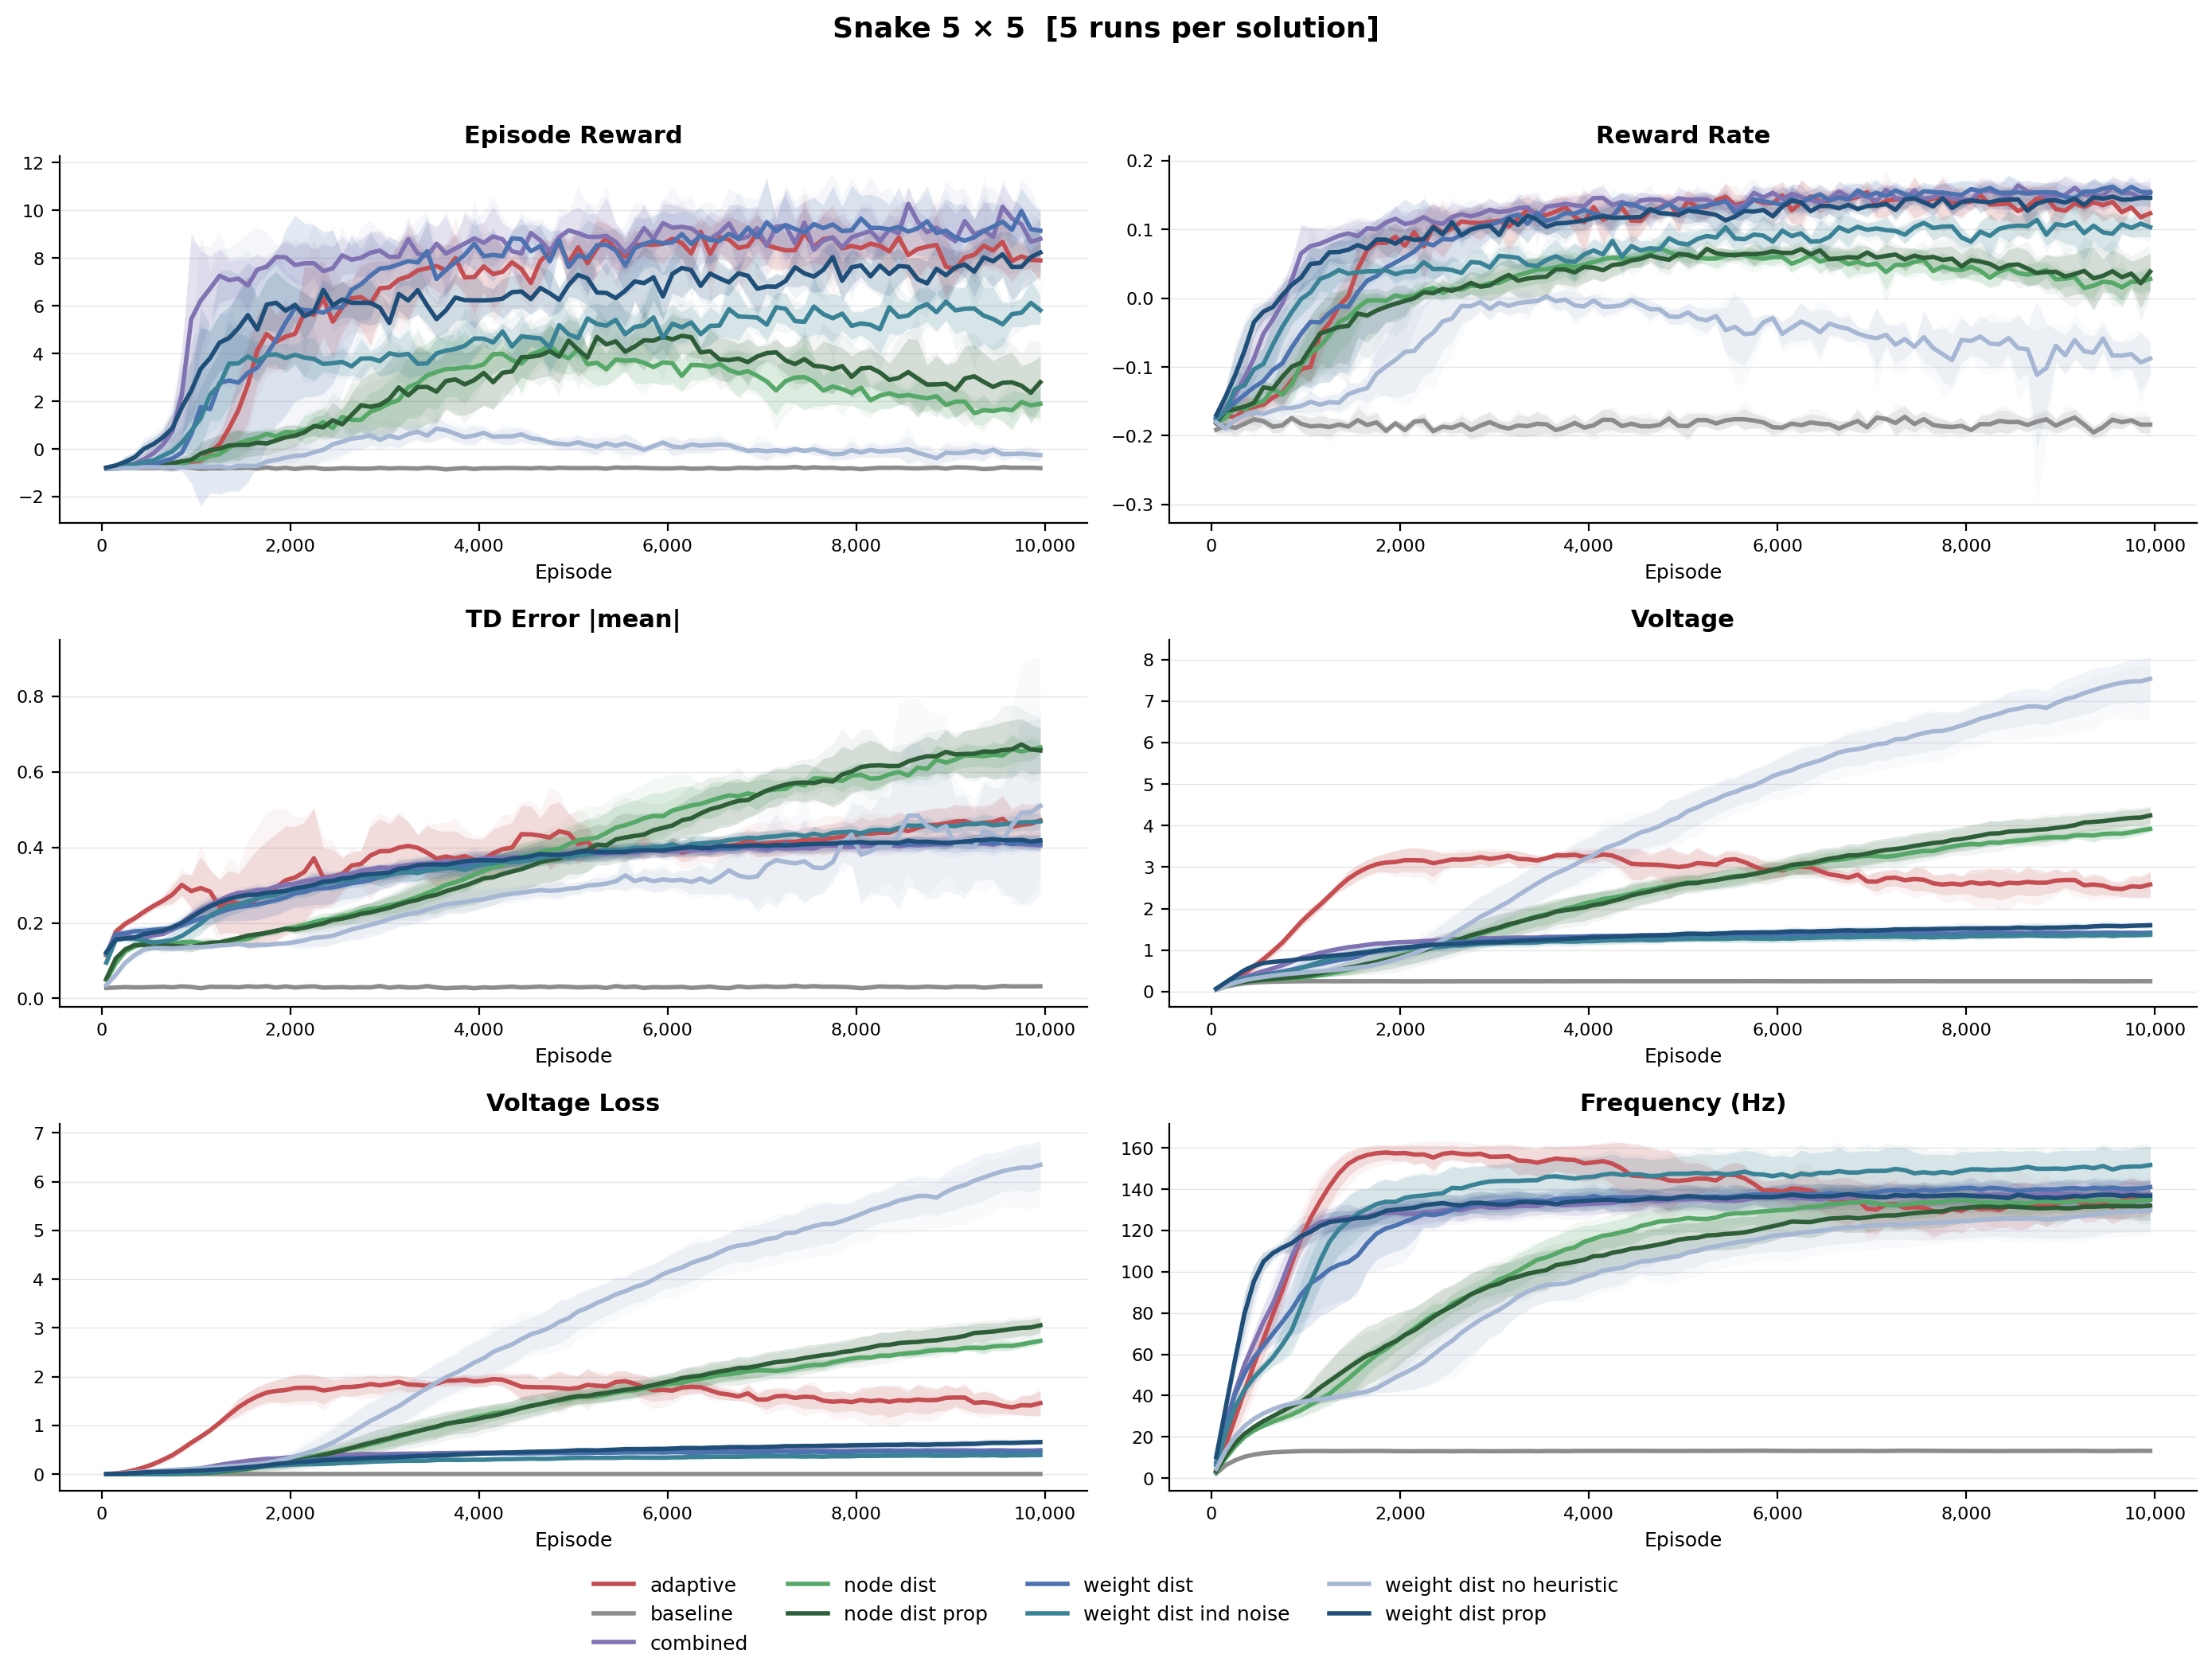
\includegraphics[width=\linewidth]{images/SnakeComparison.png}
    \end{column}
  \end{columns}
\end{frame}

\begin{frame}{Performance comparison on Snake $5\times5$}

      With \textbf{no feedback weights at all}, distributed variants reach, and arguably surpass, the
      same operating point as \aeprop{}.

      Near the ceiling for this
      small-$\gamma$   regime.

      The \emph{combined} is the fastest to reach the top, and maintains it during learning, y observing the dynamics it seems to behave more closely to distributed e-prop.
      \vfill
  \begin{columns}[T]
    \begin{column}{0.8\textwidth}
      \centering
      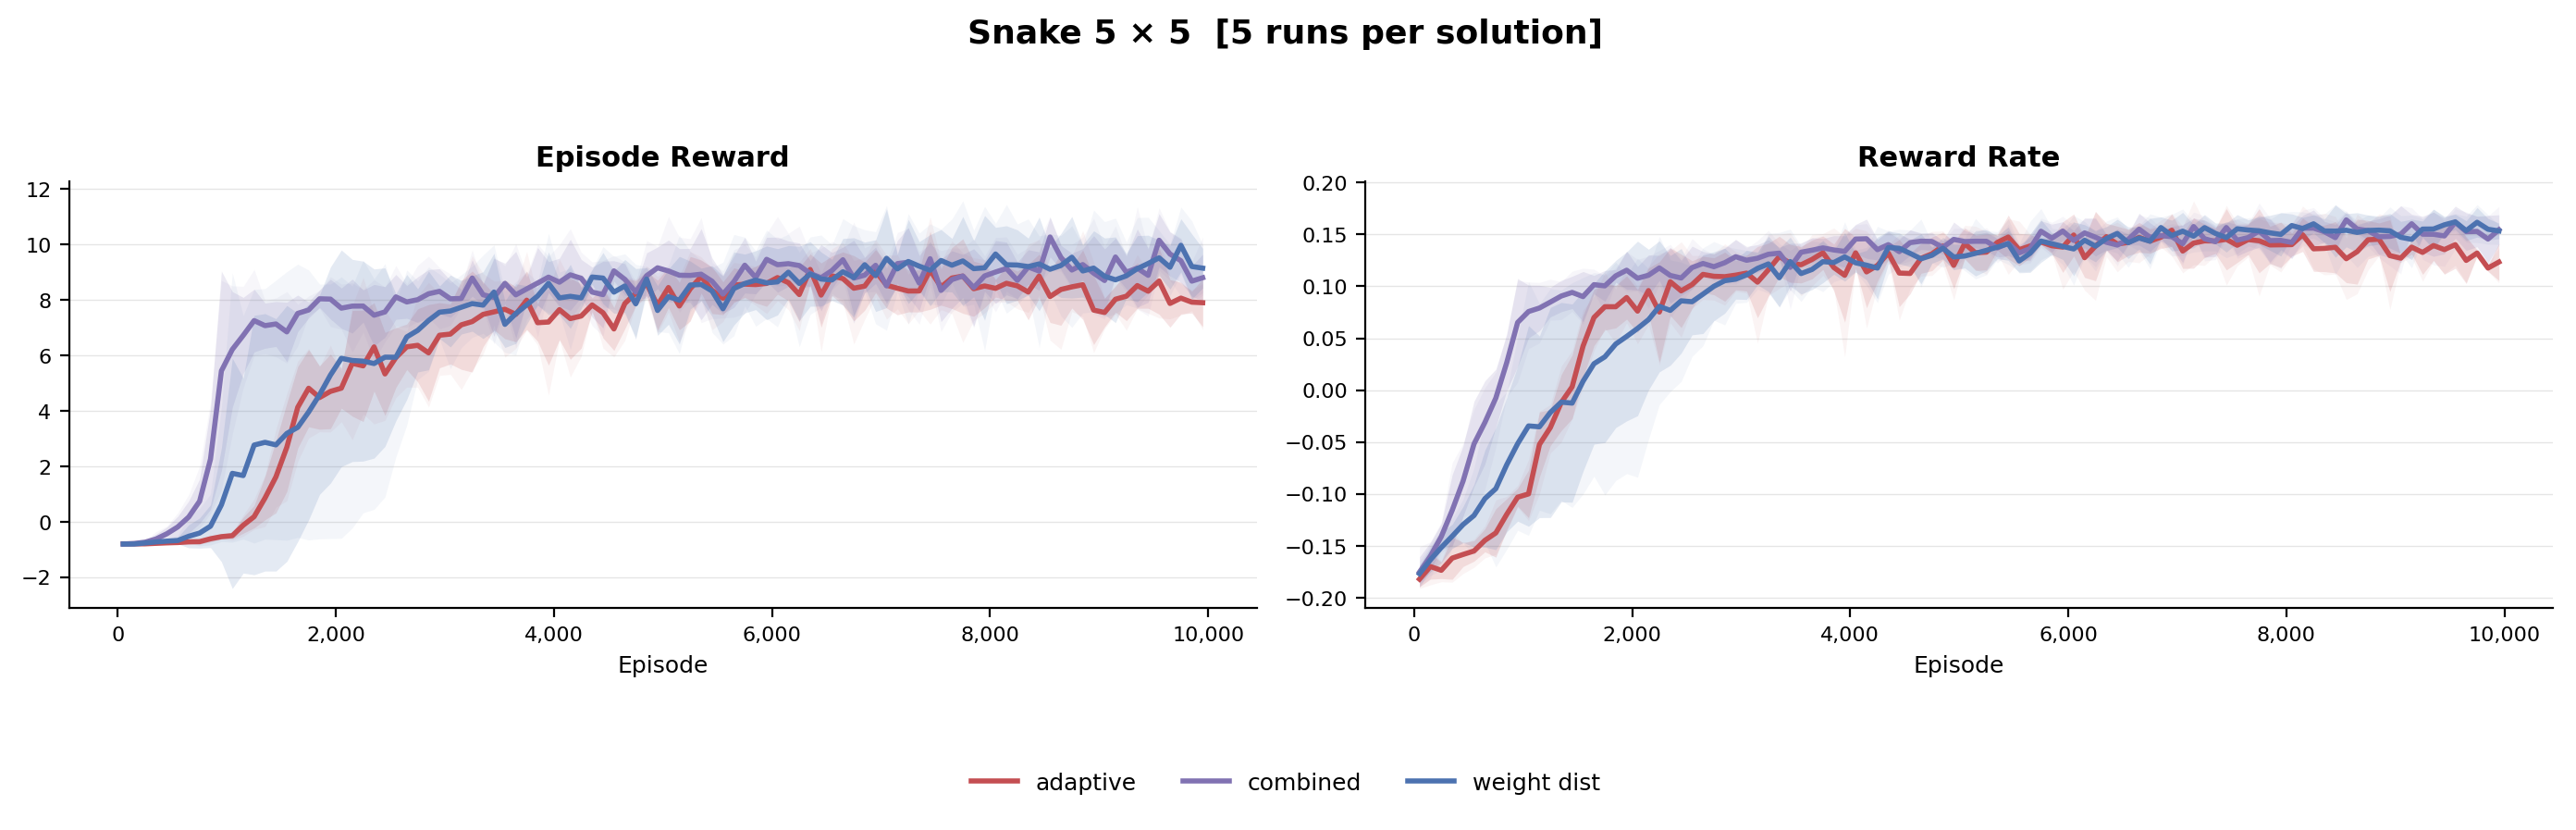
\includegraphics[width=\linewidth]{SnakeTop3Comparison.png}
    \end{column}
  \end{columns}
\end{frame}

\begin{frame}{$\lambda$-robustness on Snake $5\times5$}
      Sweeping the credit horizon $\lambda$ on Snake: \aeprop{} tolerates nearly
      the full range, failing only at the most extreme value.
      \vfill
      The distributed variant has a narrower band of $\lambda$
      for which it learns promptly.
      \vfill
      \small (The ordering reverses on Pac-Man, see later.)
  \begin{columns}[T]
    \begin{column}{0.7\textwidth}
      \centering
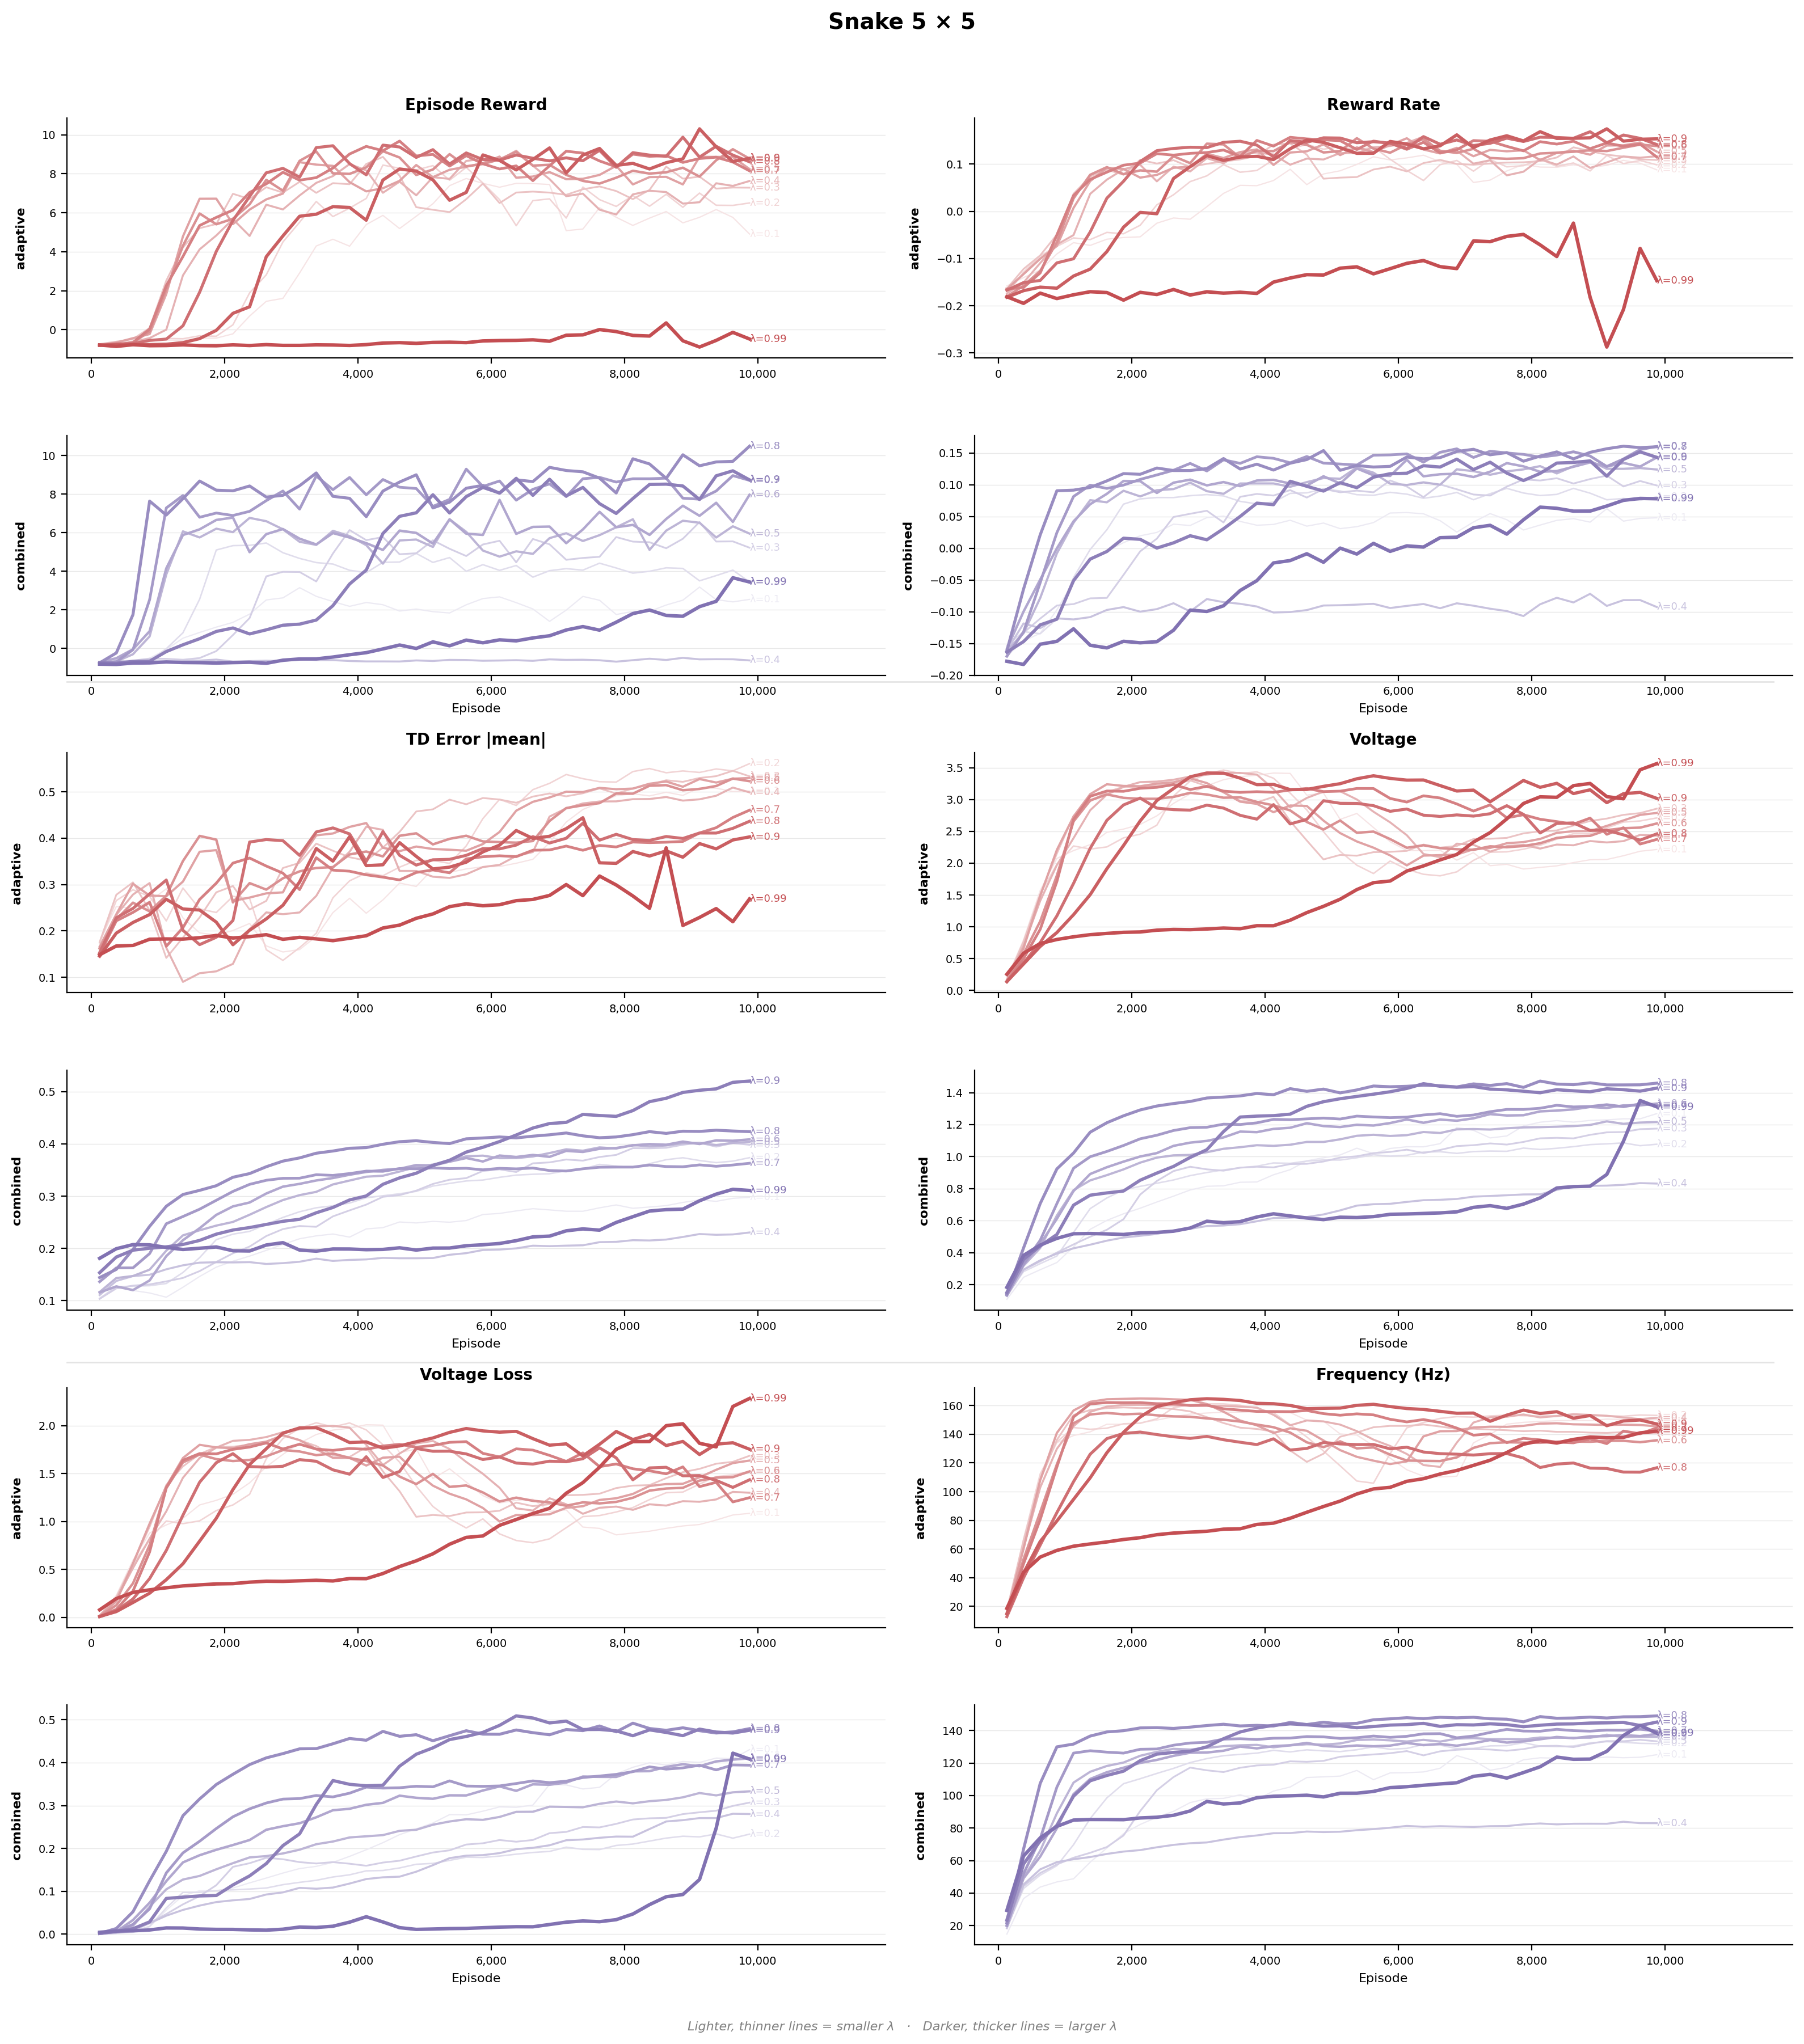
\includegraphics[width=\linewidth,clip,trim=0 29cm 0 0]{images/SnakeLambdaComparison.png}
    \end{column}
  \end{columns}
\end{frame}


\begin{frame}{$\lambda$-robustness on Snake $5\times5$}
  \begin{columns}[T]
    \begin{column}{0.3\textwidth}
      The adaptive variant seems more unstable in both the sweep and in individual runs. 
      
      Combined seems show clear patterns with regards to the choice of lambda. 
      
      \end{column}
    \begin{column}{0.63\textwidth}
      \centering
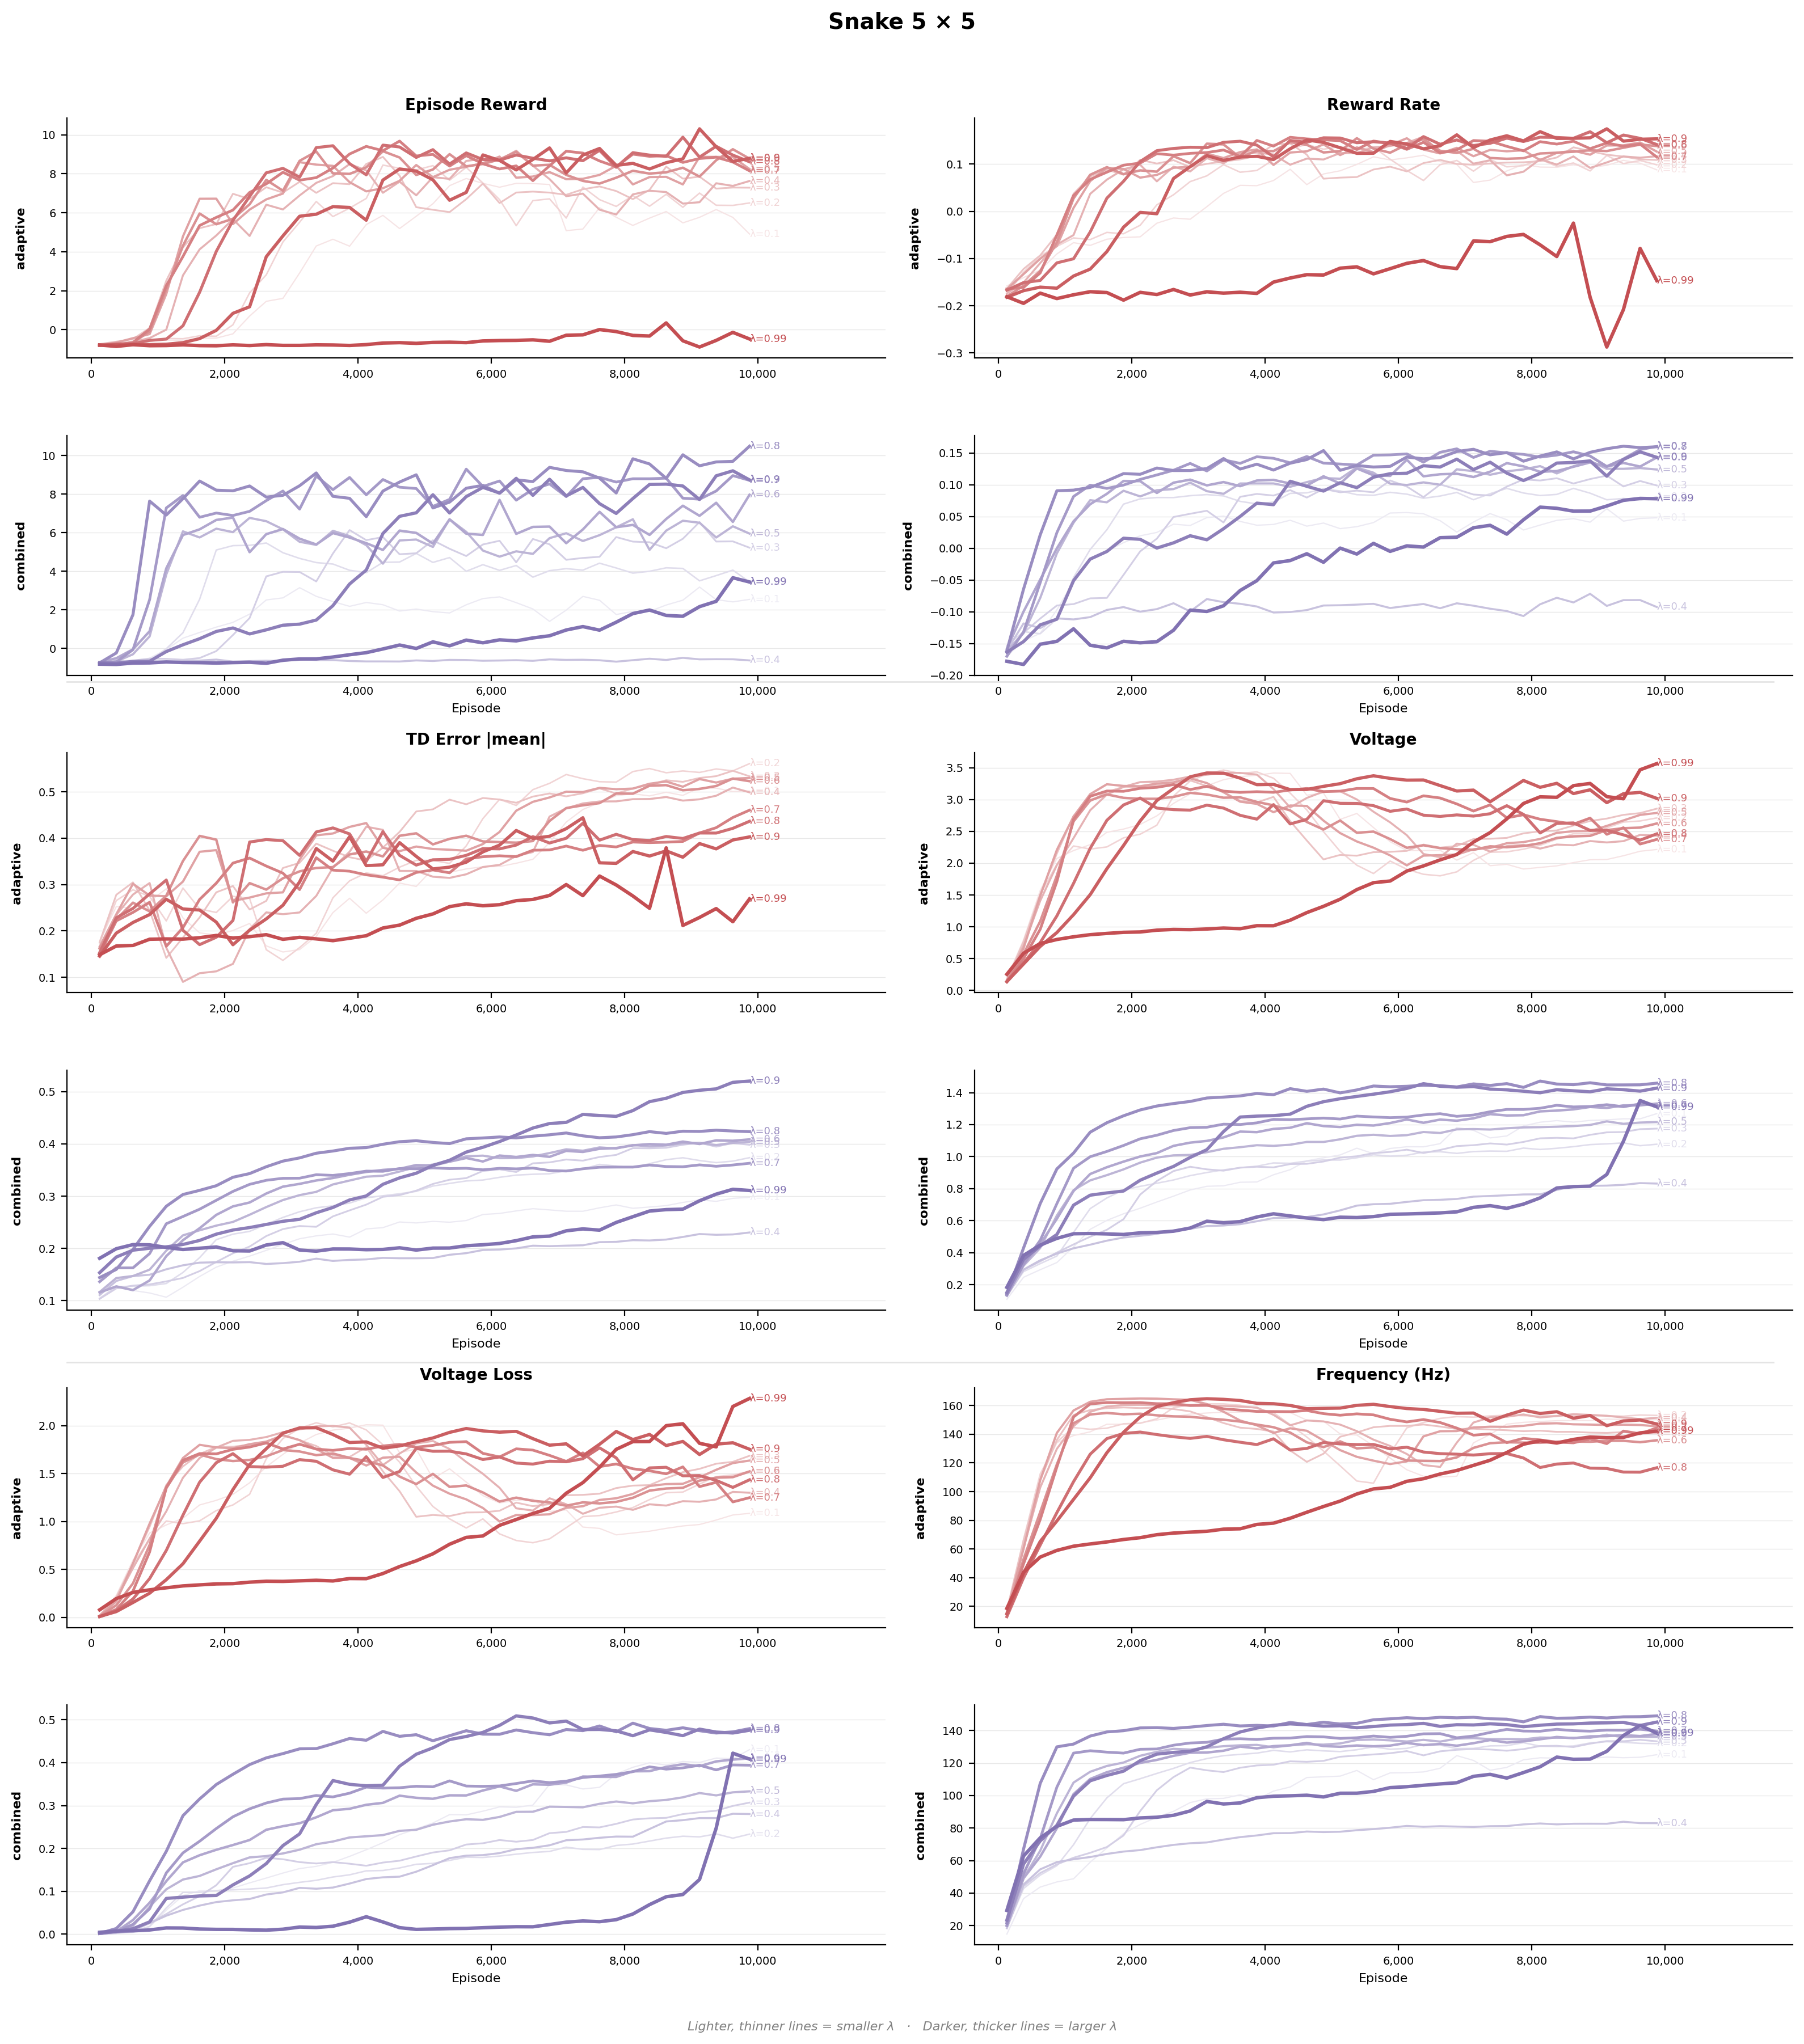
\includegraphics[width=\linewidth,clip,trim=0 0 0 16cm]{images/SnakeLambdaComparison.png}
    \end{column}
  \end{columns}
\end{frame}

\begin{frame}{Depth comparison on Snake $5\times5$}
      At a \emph{fixed} training budget, distributed e-prop looks more
      \textbf{depth-robust} than adaptive: performance degrades more gracefully
      as layers are added.
      \vfill
      \small This alone would suggest distributed e-prop scales better with
      depth, but it's not the full picture.

  \begin{columns}[T]
    \begin{column}{0.7\textwidth}
      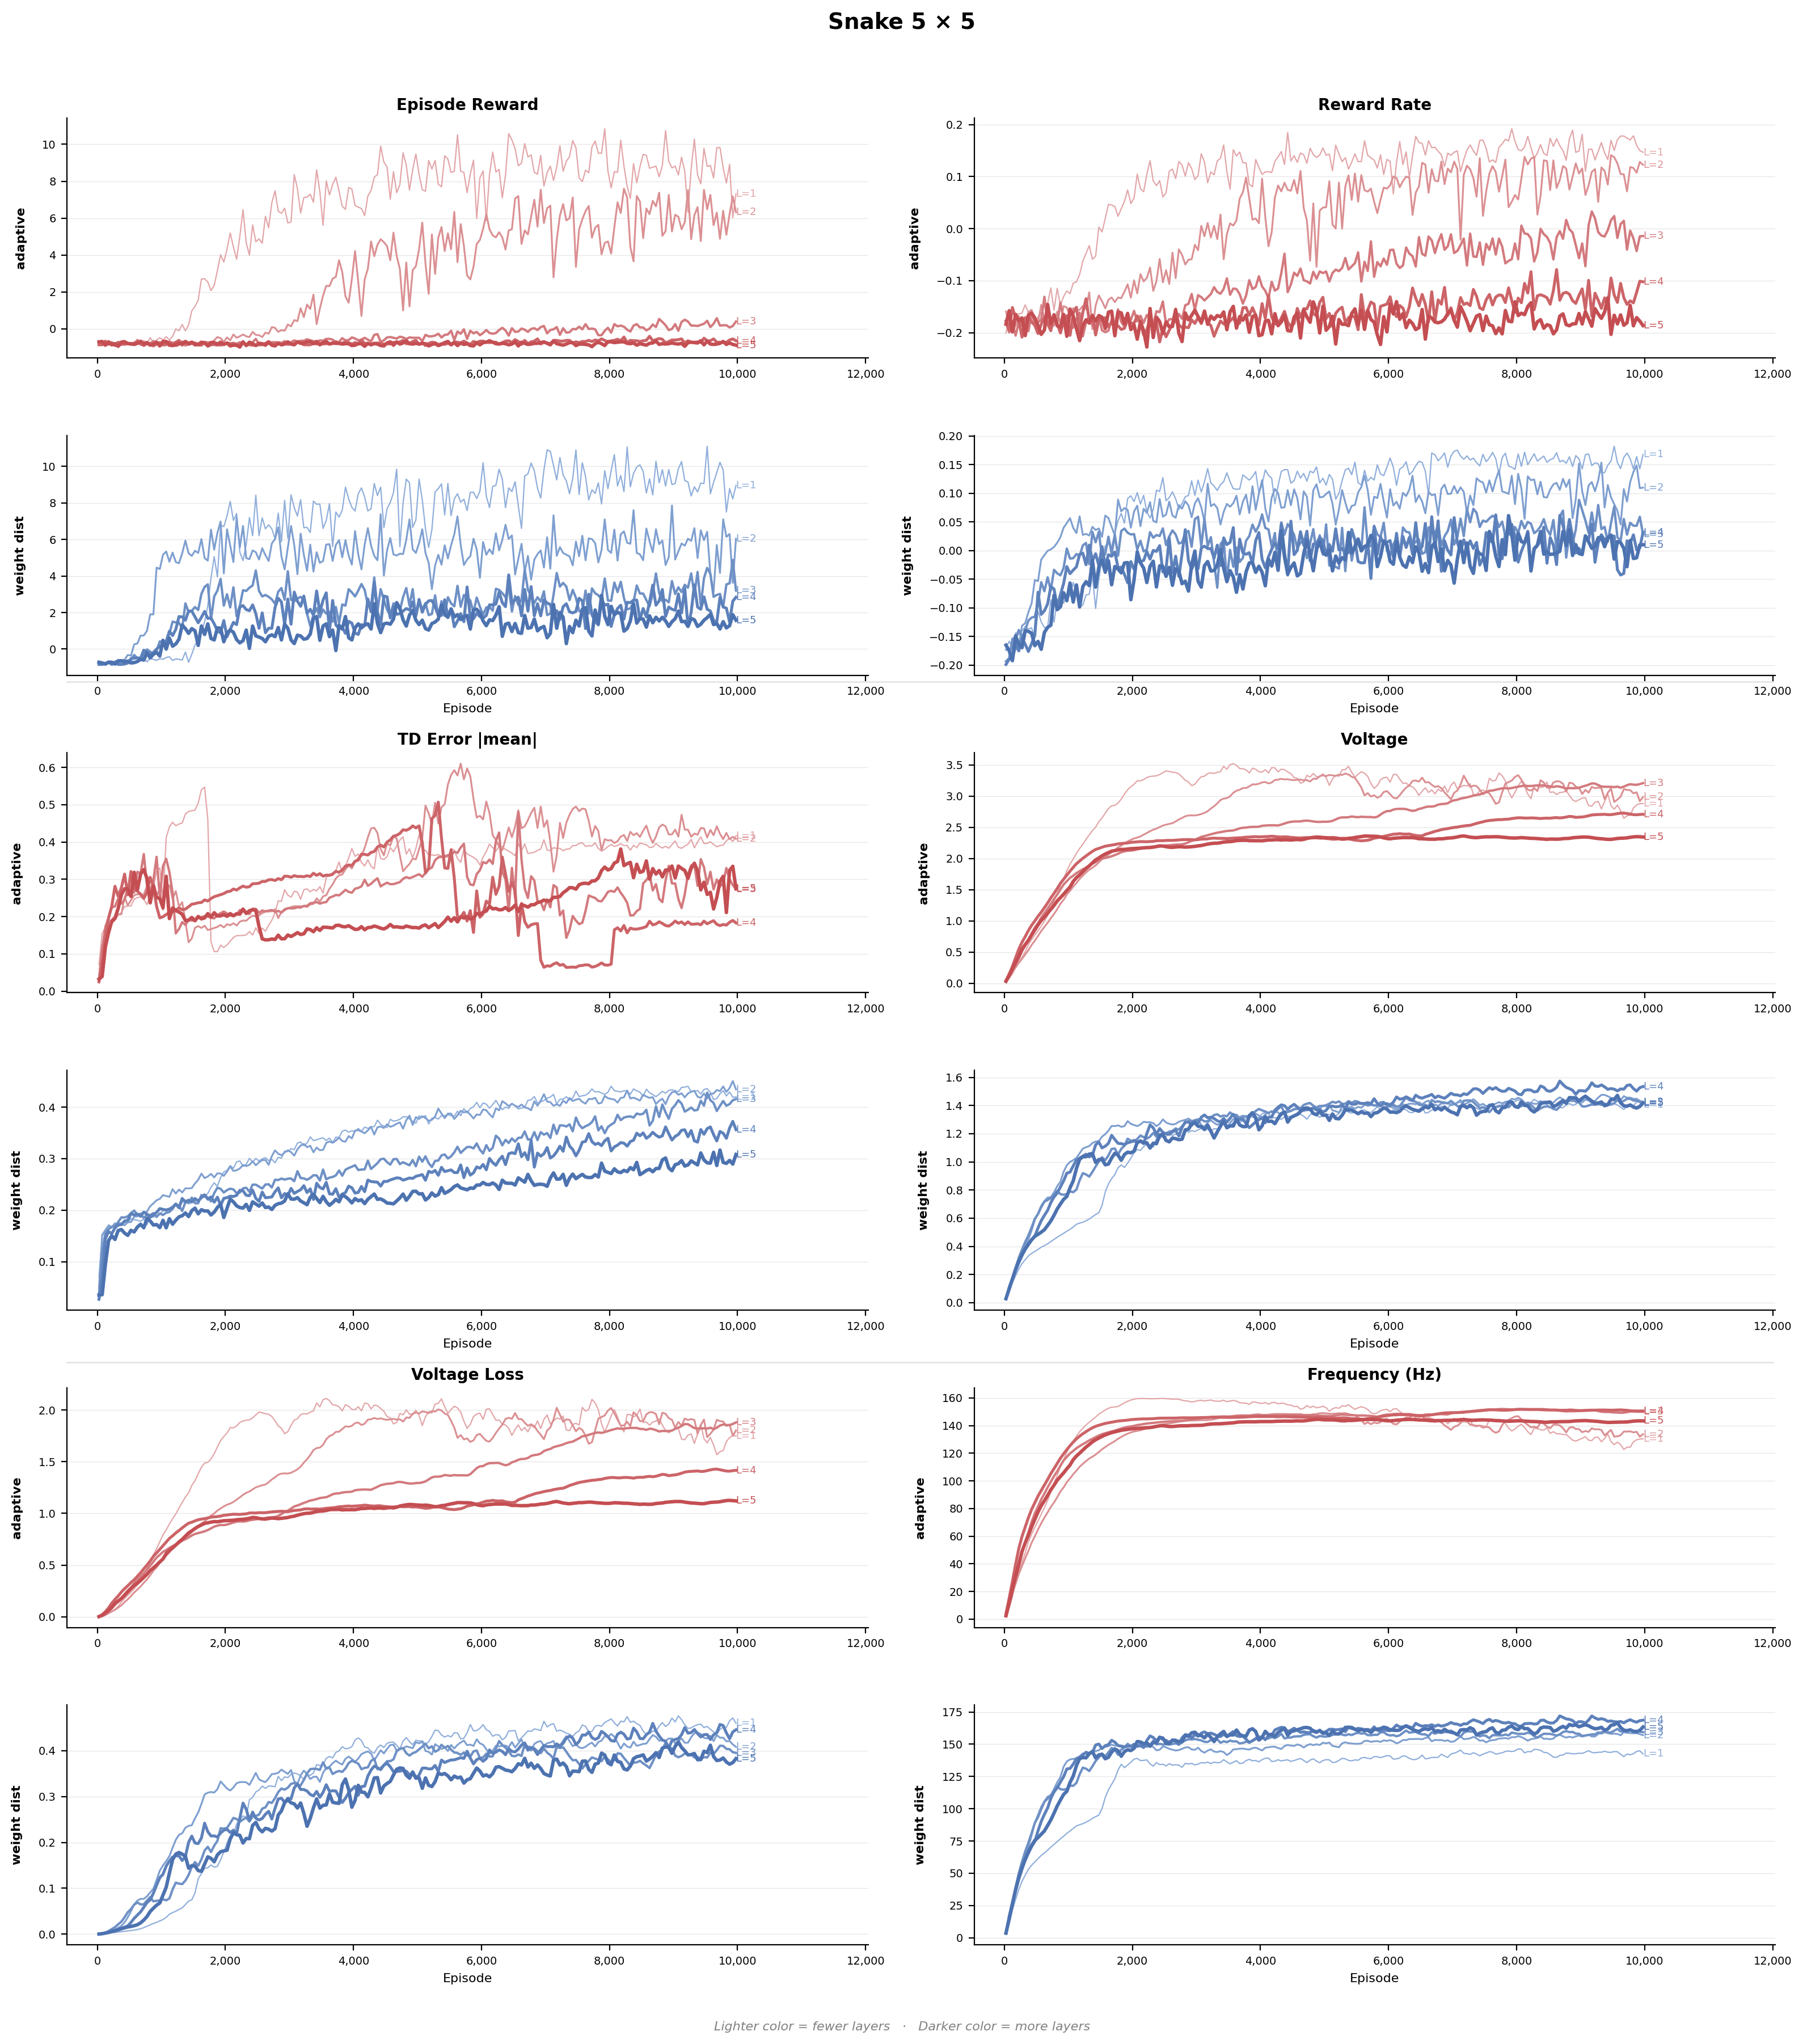
\includegraphics[width=\linewidth,clip,trim=0 29cm 0 0]{images/SnakeLayersComparison.png}
    \end{column}
  \end{columns}
\end{frame}

\begin{frame}{Depth comparison on Snake $5\times5$}
  \begin{columns}[T]
    \begin{column}{0.48\textwidth}
      The spiking dynamics tell a sharper story than reward alone: \aeprop{}
      reaches a \textbf{higher membrane voltage} ($\sim$3) and voltage loss,
      both \textbf{rising with depth}.
      \vfill
      \deprop{} stays \textbf{low and flat} ($\sim$1.5) across every depth
      tested, with small voltage loss throughout.
      \vfill
      \small TD error grows with depth for both, but adaptive's is visibly
      noisier; firing frequency converges to a similar high band
      ($\sim$140-170\,Hz) regardless of rule or depth.
    \end{column}
    \begin{column}{0.48\textwidth}
      \centering
      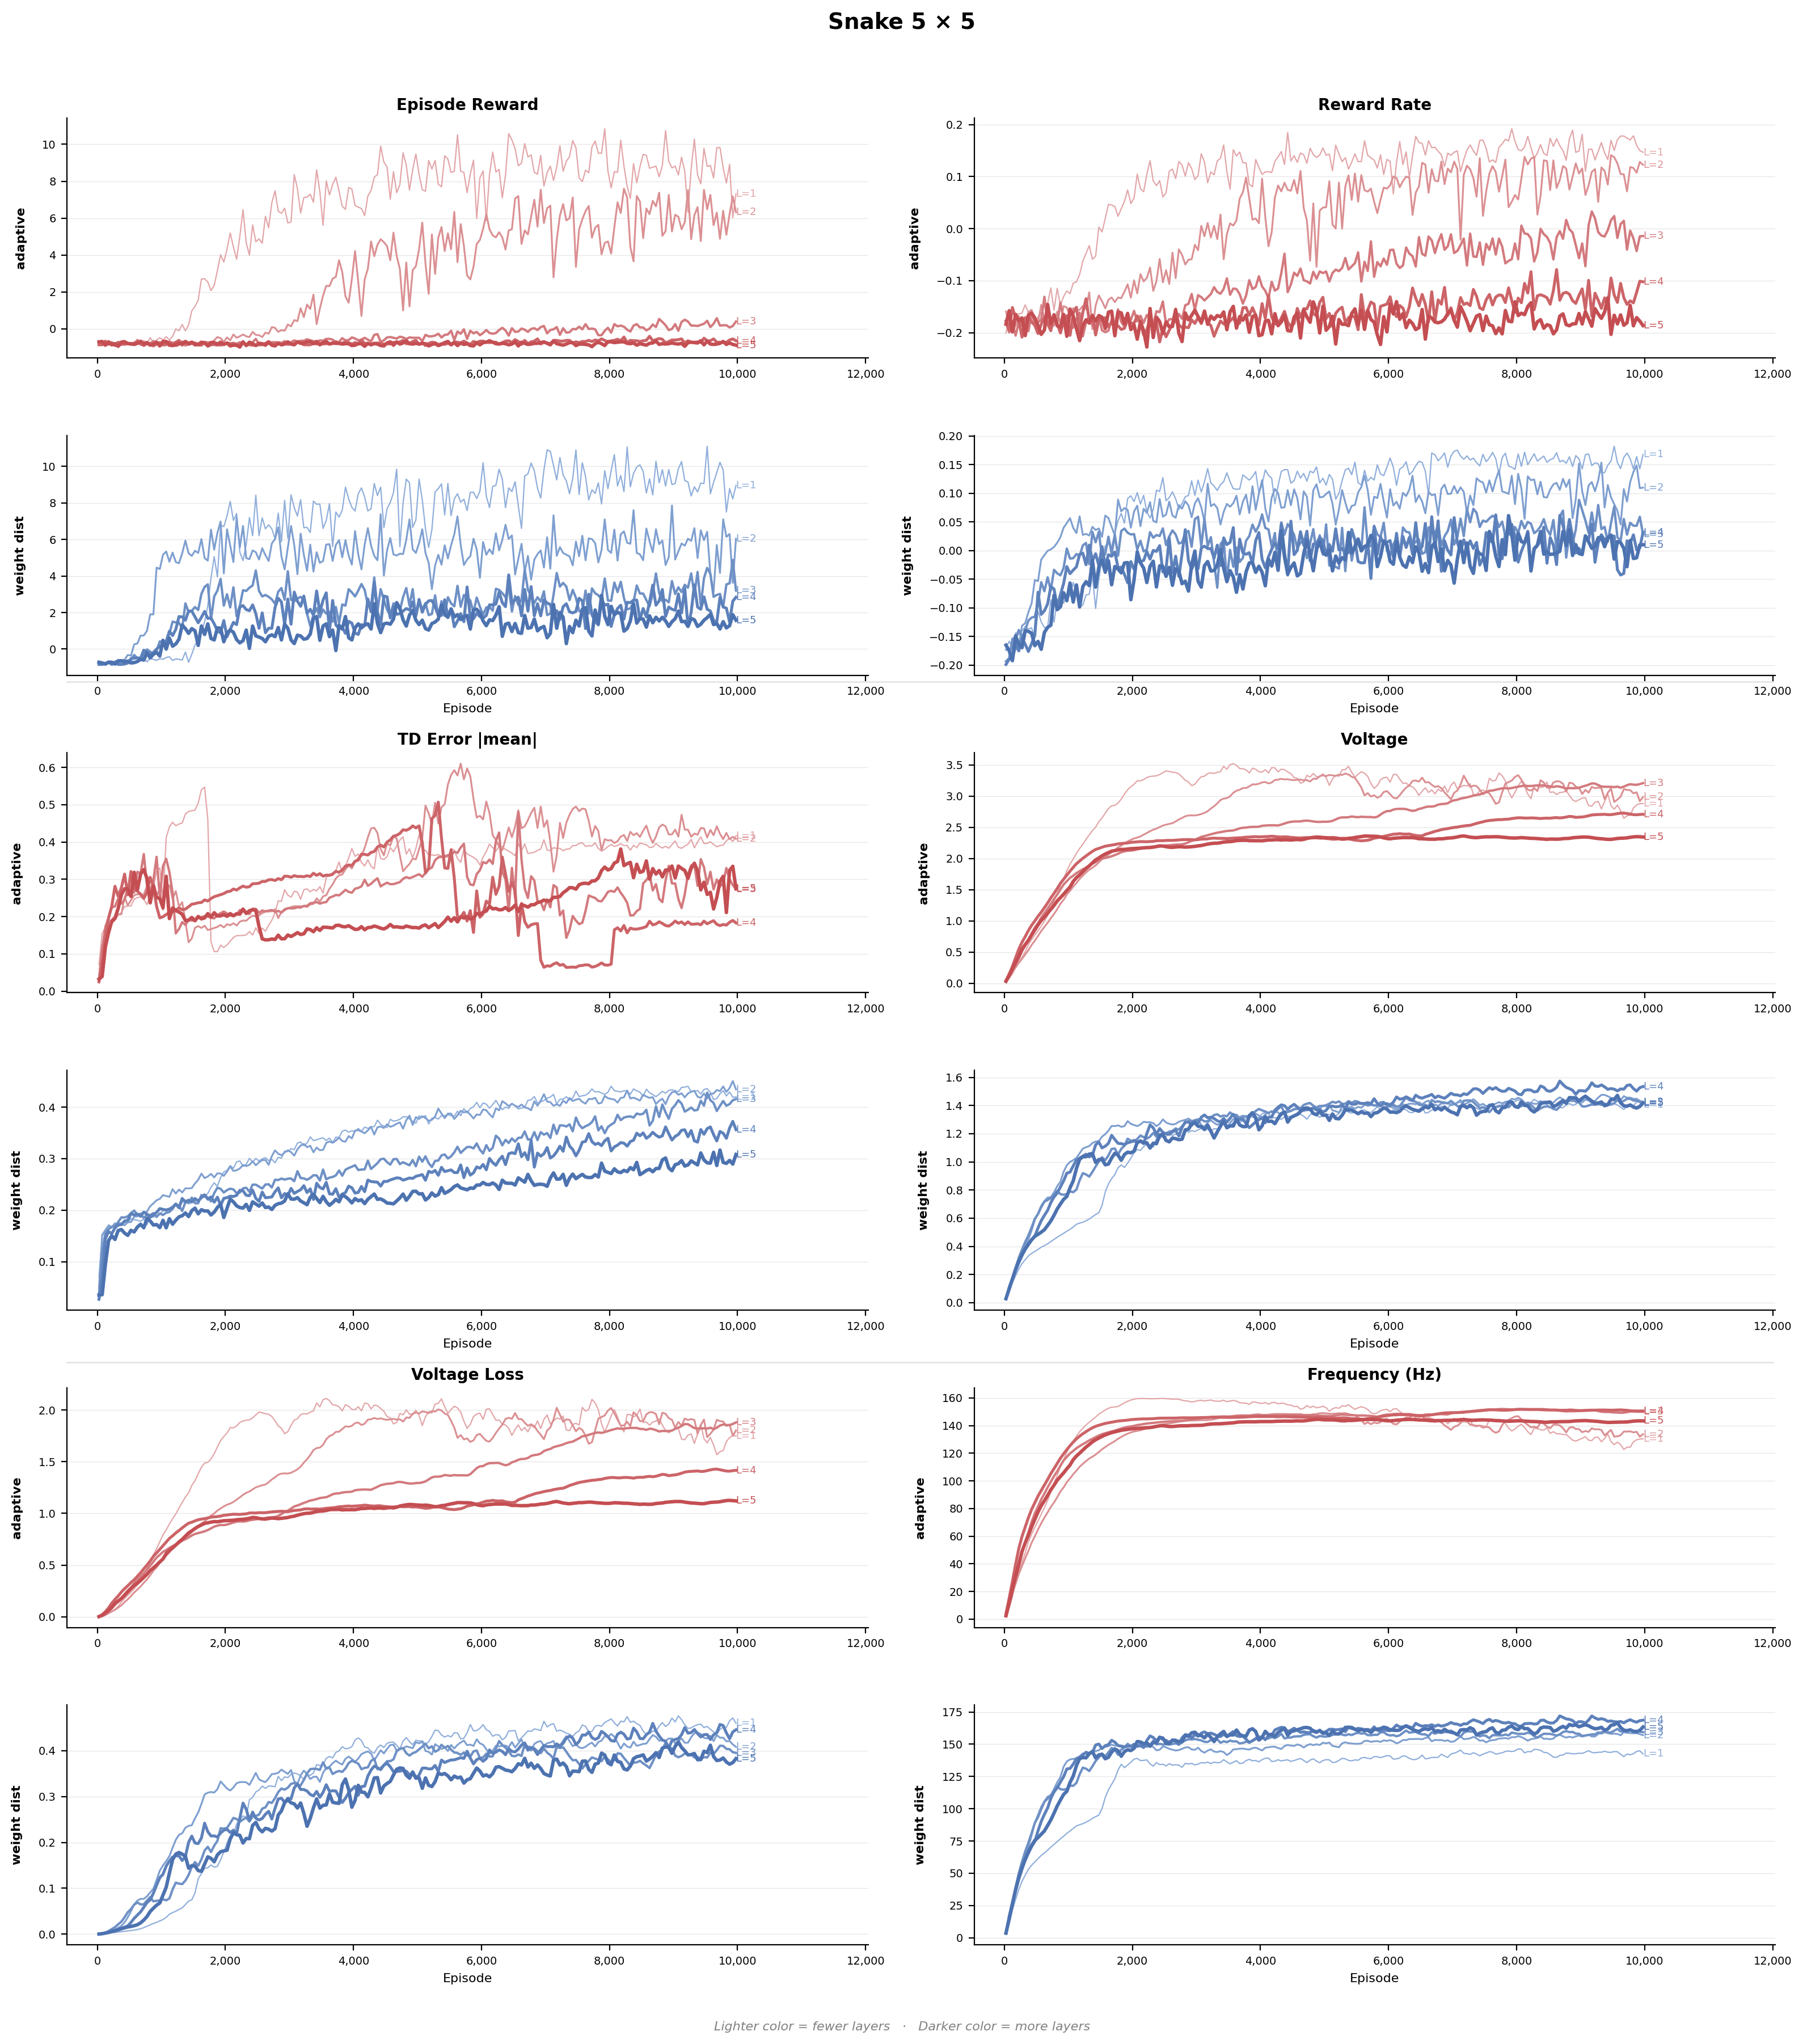
\includegraphics[width=\linewidth,clip,trim=0 0 0 16cm]{images/SnakeLayersComparison.png}
    \end{column}
  \end{columns}
\end{frame}

\begin{frame}{Depth comparison on Snake $5\times5$ with extended runs}
  \begin{columns}[T]
    \begin{column}{0.38\textwidth}
      Over a long ($\sim$100k-episode) 5-layer run, \aeprop{} starts slowly
      (feedback alignment) then \textbf{overtakes} the distributed variants,
      which plateau early.
      These executions where done by updating the parameters per episode and not per action.
      \vfill
      \small Depth-robustness seems to be a budget artifact, but it is clear that 
      depth affects the two rules differently.
    \end{column}
    \begin{column}{0.6\textwidth}
      \centering
      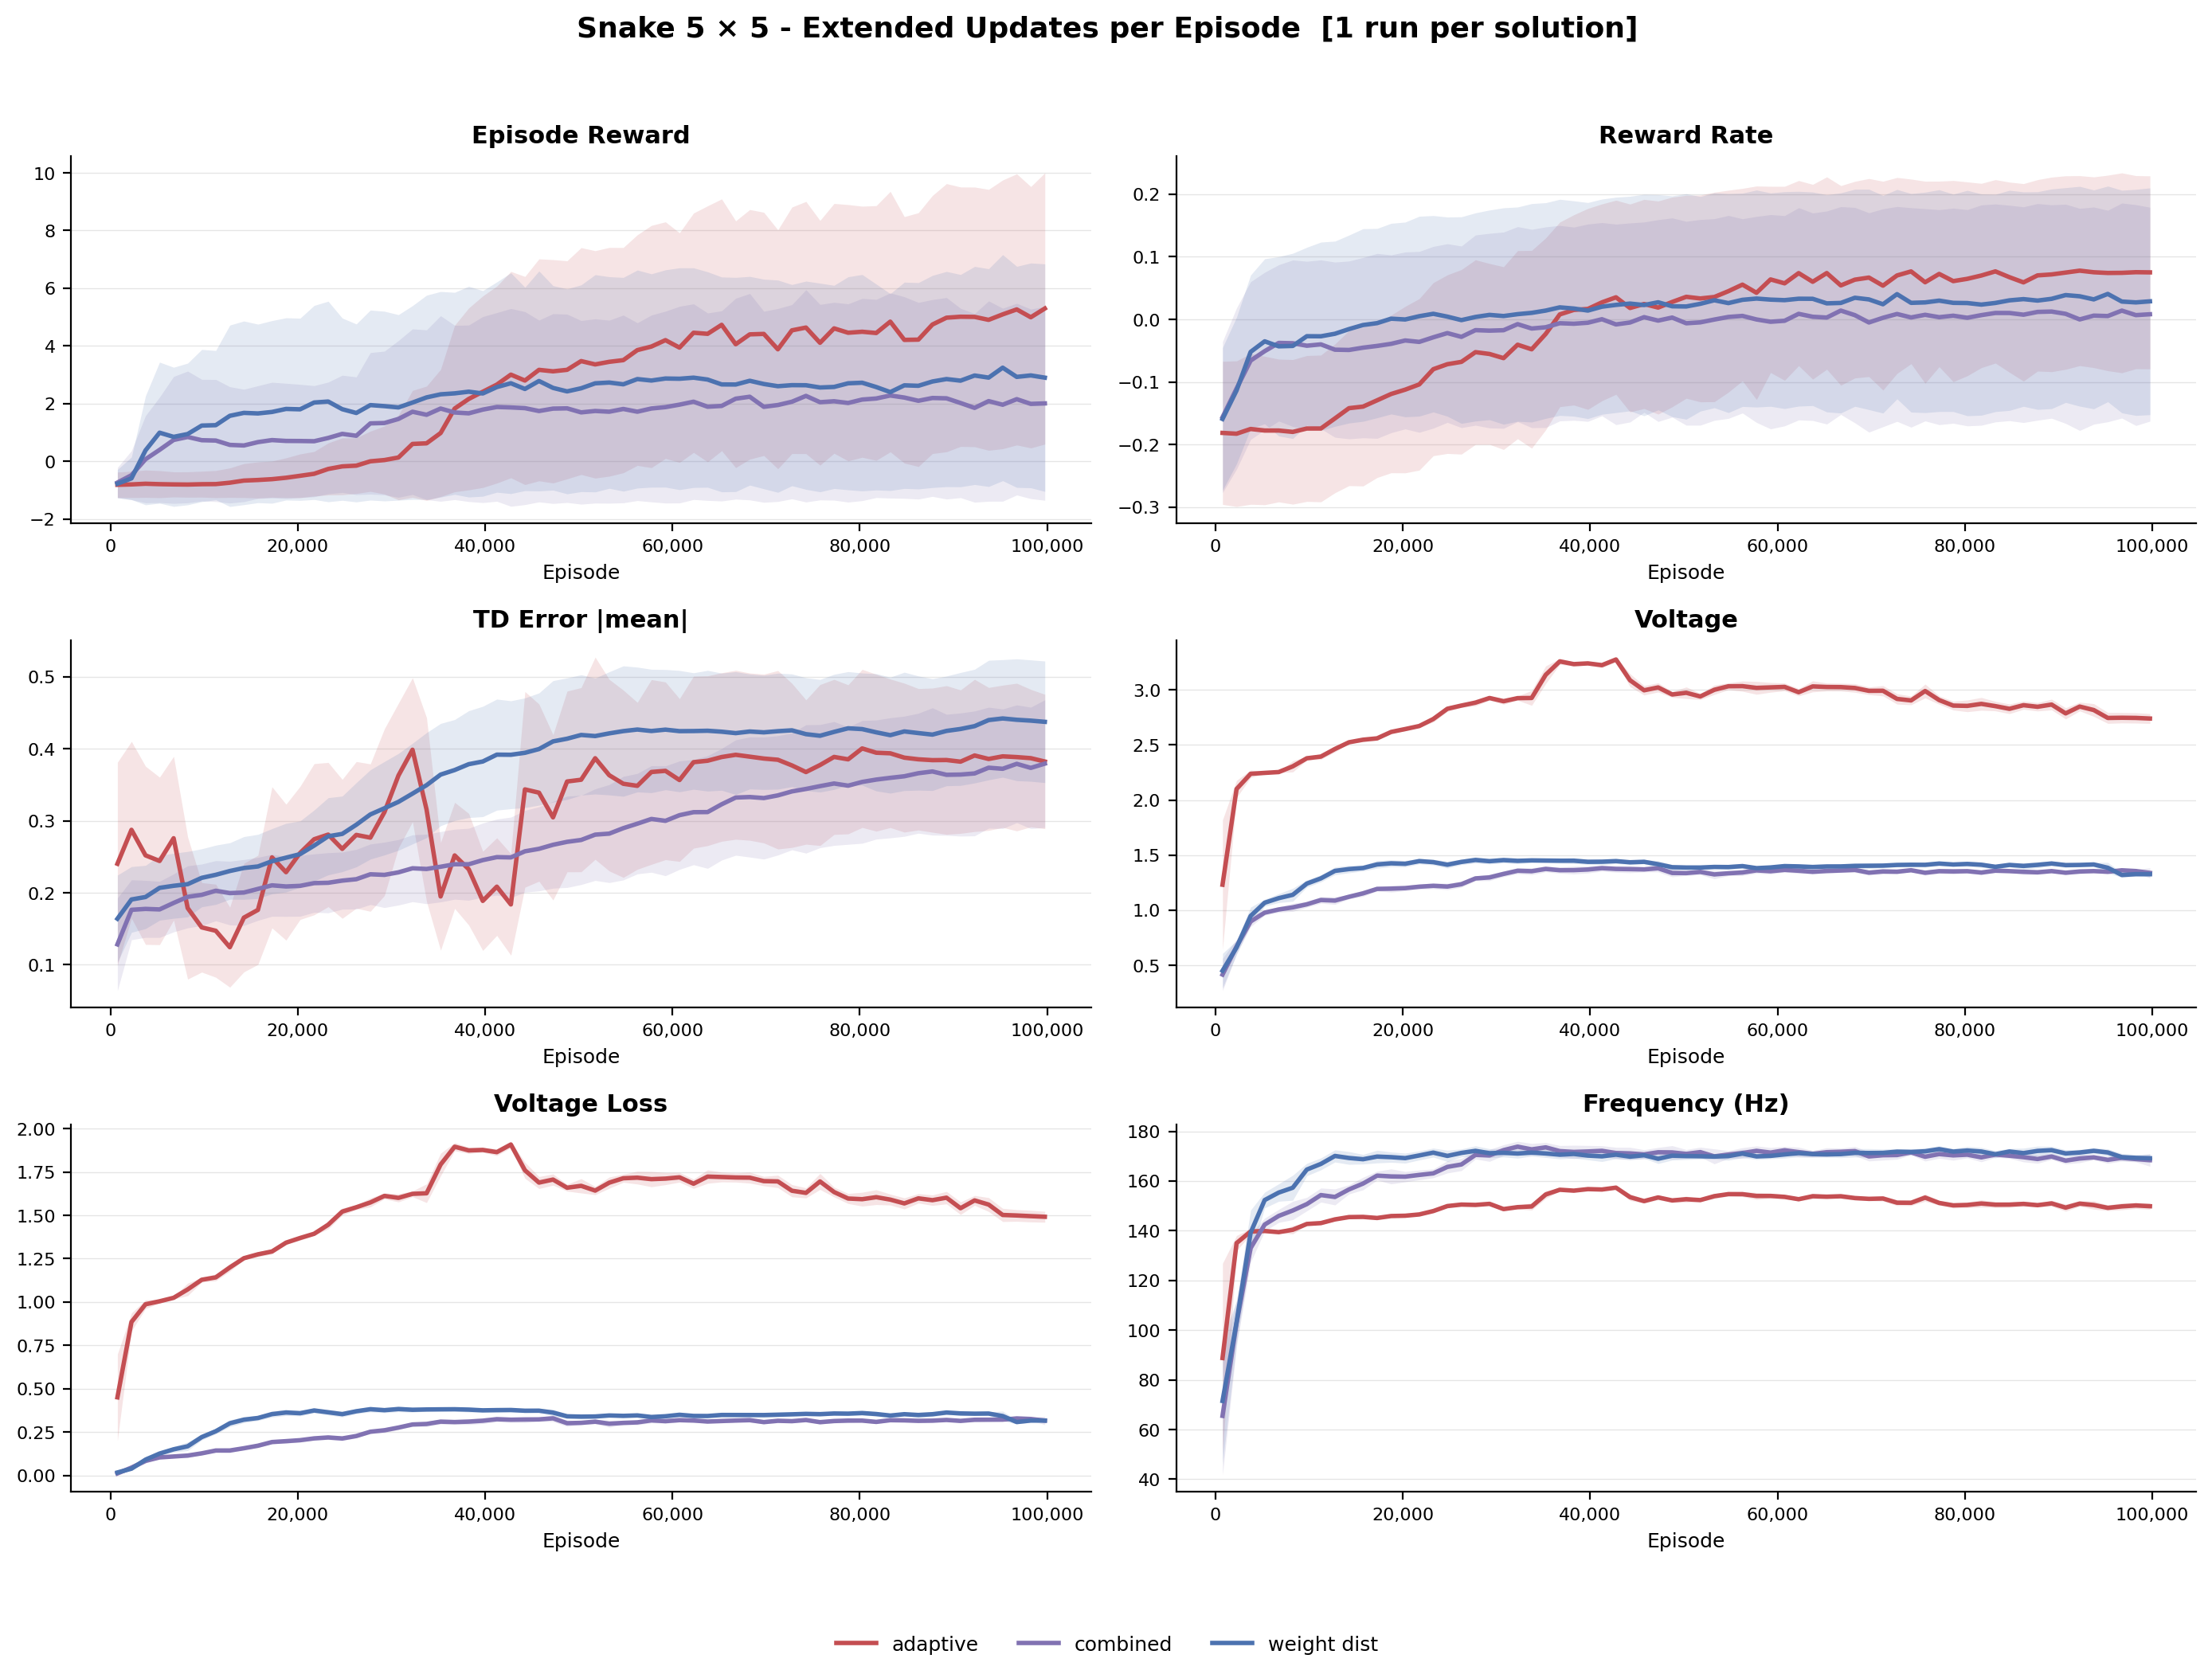
\includegraphics[width=\linewidth]{images/comparison_extended_updates_per_episode_1_runs.png}
    \end{column}
  \end{columns}
\end{frame}

\begin{frame}{Local reward-based regularization on Snake $5\times5$}
  \begin{columns}[T]
    \begin{column}{0.38\textwidth}
      A local, perturbation-gated \textbf{voltage reward} keeps membranes
      well-regulated for distributed e-prop, the same term \emph{diverges}
      under standard e-prop.
      \vfill
      \begin{itemize}\small
        \item Locality could explain why voltage regularization works well.
        \item Frequency regularization is harder.
        \item Regularization strength seems to degrade this task performance.
      \end{itemize}
    \end{column}
    \begin{column}{0.6\textwidth}
      \centering
      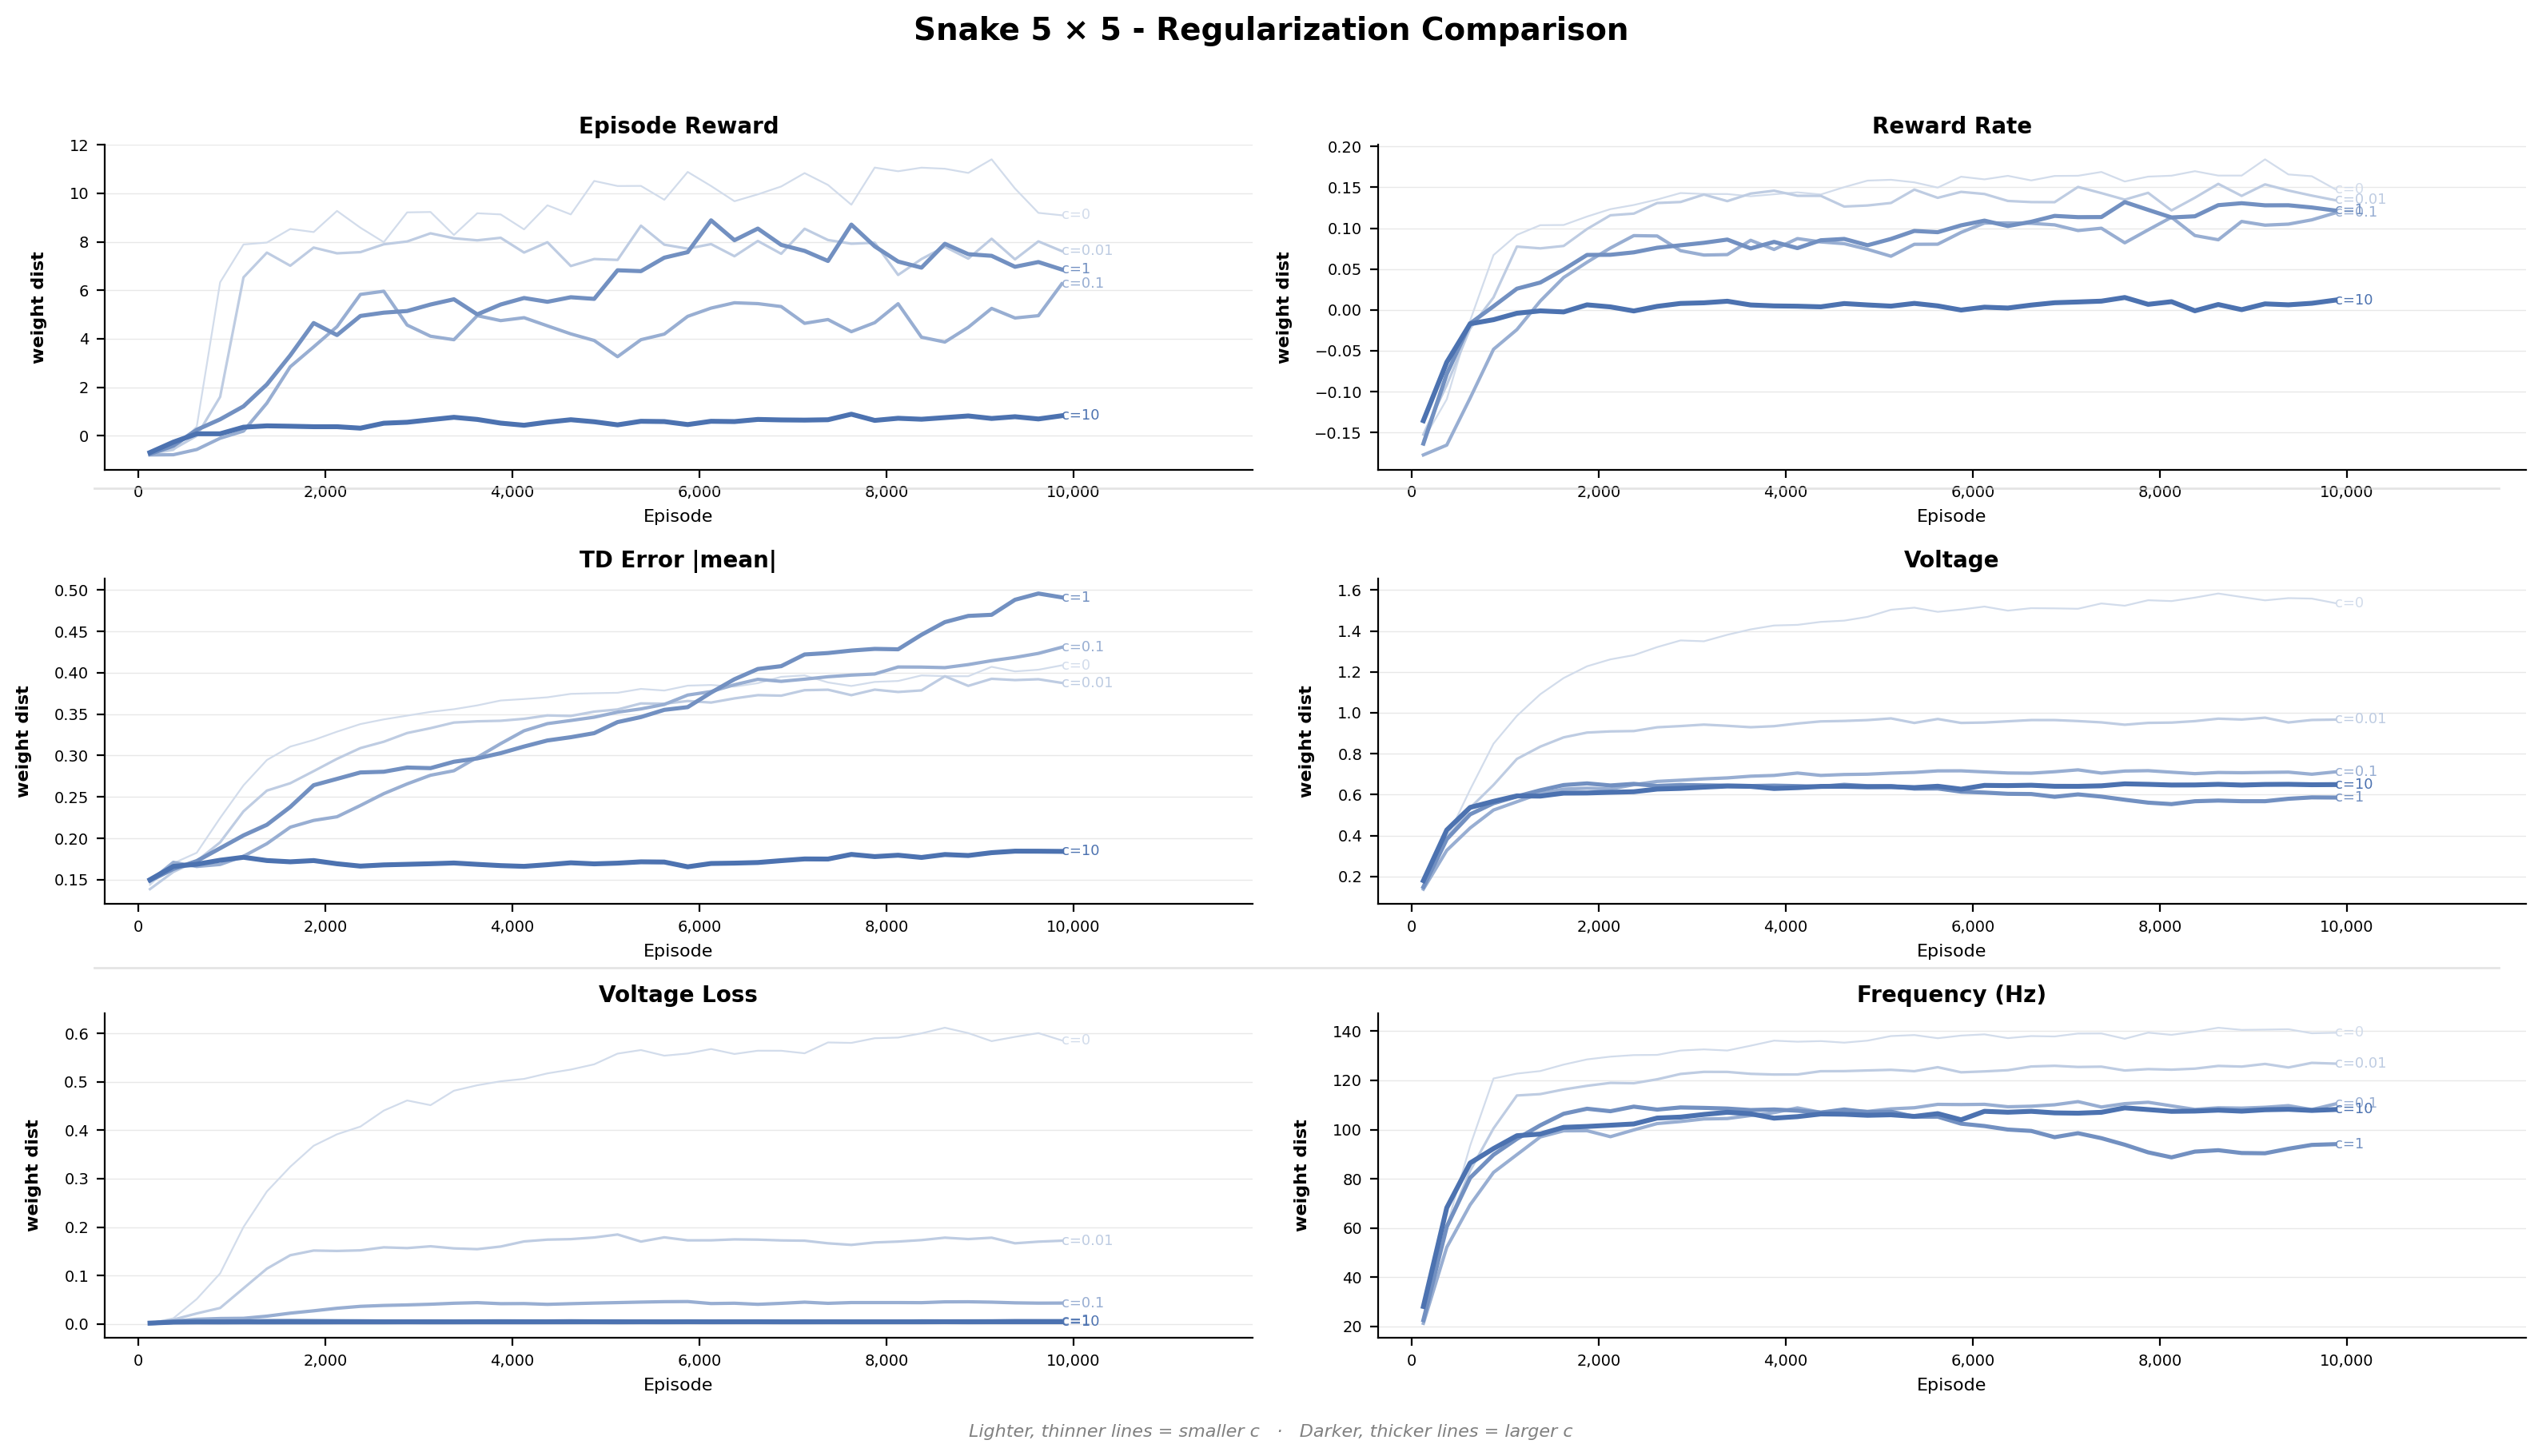
\includegraphics[width=\linewidth]{images/SnakeRegularizationComparison.png}
    \end{column}
  \end{columns}
\end{frame}

% ---- 6. A surprise: cleaner value representations ------------
\begin{frame}{Distributed e-prop surprisingly cleaner value representations}
  \begin{columns}[T]
    \begin{column}{0.28\textwidth}
      Distributed e-prop carries \emph{no} information about the value
      function, yet its representations have consistently been observed to let the value head regress faster and
      more cleanly than adaptive e-prop's.
      \vfill
      \small Useful representations for the value head apparently do not need explicit value gradient.
    \end{column}
    \begin{column}{0.7\textwidth}
      \centering
      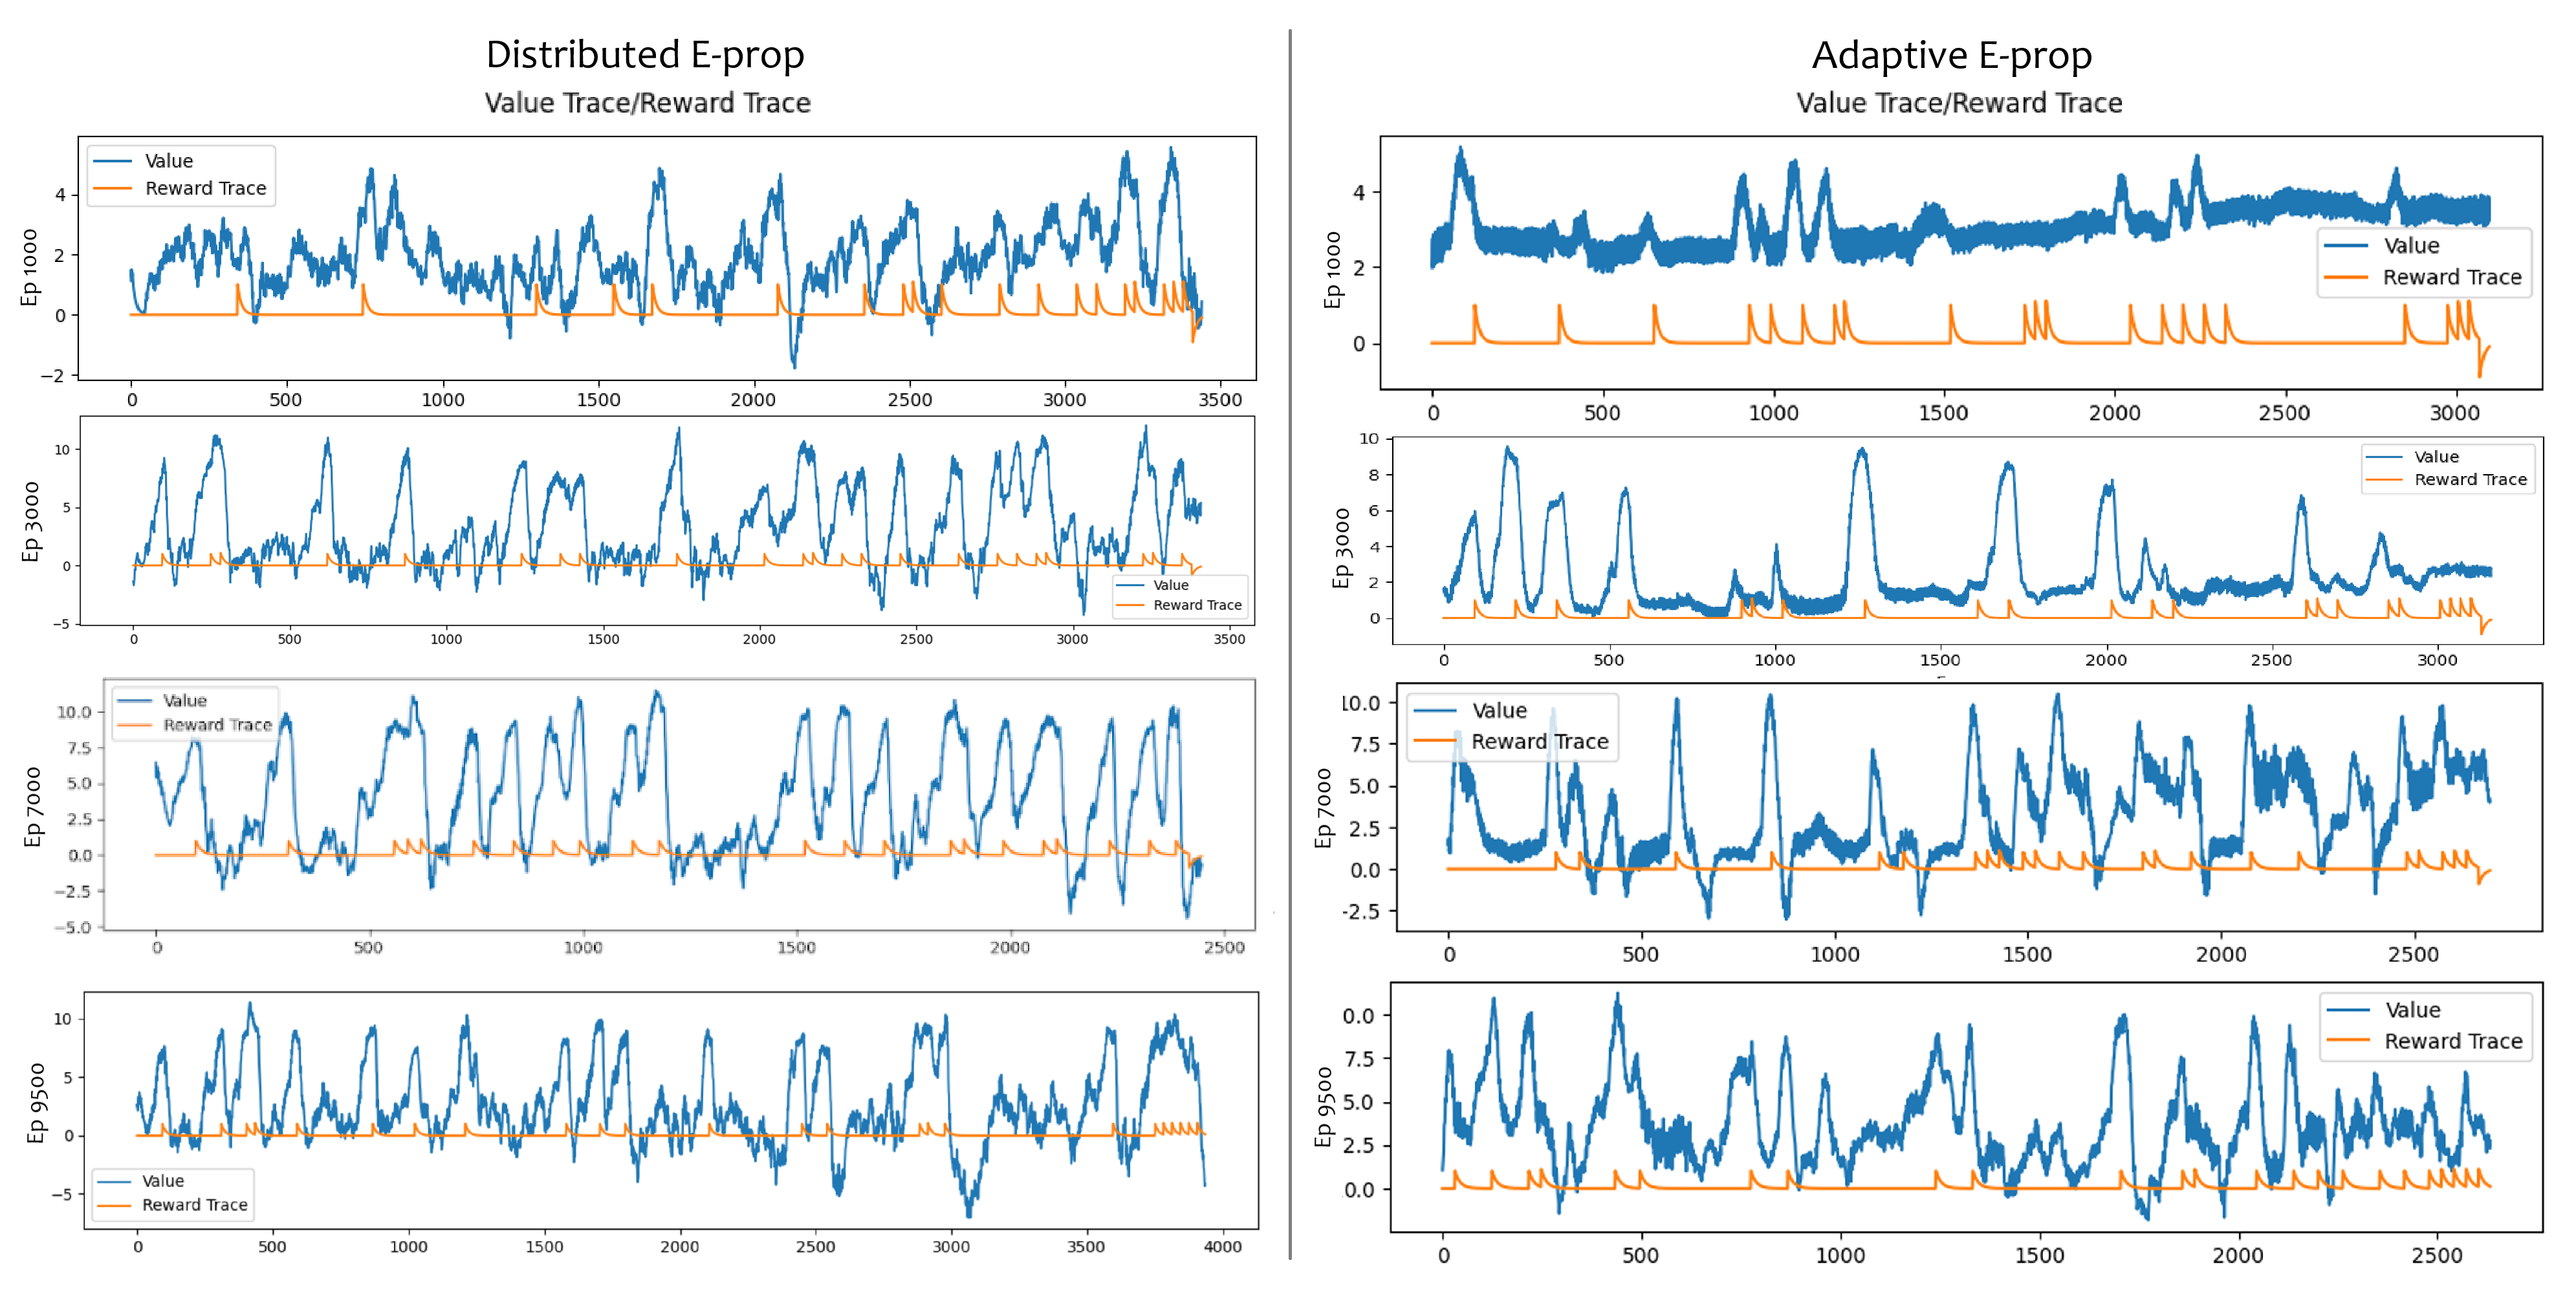
\includegraphics[width=\linewidth]{images/SnakeValueTraceComparison.png}\\
      {\scriptsize Value (blue) tracks the reward trace more sharply for
       distributed e-prop, earlier in training.}
    \end{column}
  \end{columns}
\end{frame}

\begin{frame}{Best individual runs on Snake $5\times5$}
  \scriptsize
  \setlength{\tabcolsep}{6pt}\renewcommand{\arraystretch}{1.1}
  \begin{tabular}{l r r r r}
    \toprule
    Run & Best100 RewardRate & Best100 Score & Wins & Win\% \\
    \midrule
    \emph{symmetric}                  & \textbf{0.2113} & \textbf{12.65} & 14 & 14\% \\
    weight dist creg 0 (Reg)          & 0.1897 & 12.31 & \textbf{33} & \textbf{33\%} \\
    weight dist (4)                   & 0.1823 & 11.82 & 11 & 11\% \\
    weight dist (3)                   & 0.1776 & 11.73 & 8  & 8\%  \\
    combined (3)                      & 0.1868 & 11.60 & 13 & 13\% \\
    combined $\lambda{=}0.8$          & 0.1761 & 11.56 & 8  & 8\%  \\
    combined (5)                      & 0.1826 & 11.51 & 14 & 14\% \\
    combined (1)                      & 0.1792 & 11.45 & 6  & 6\%  \\
    adaptive $\lambda{=}0.9$          & 0.1858 & 11.21 & 3  & 3\%  \\
    adaptive (4)                      & 0.1795 & 11.13 & 14 & 15\% \\
    combined (2)                      & 0.1816 & 11.01 & 11 & 11\% \\
    adaptive (3)                      & 0.1844 & 10.65 & 11 & 11\% \\
    \bottomrule
  \end{tabular}
  \vspace{0.5em}
  
  \footnotesize \emph{symmetric} tops the table, but the no-regularization
  \emph{weight dist} run wins $2.36\times$ as often and nearly matches it. The
  two best non-symmetric runs are both \emph{weight dist}, higher-variance
  exploration might explain finding stronger strategies. (Top 12 of 26; full table in thesis.)
\end{frame}

\begin{frame}{Distributed vs.\ adaptive on Pac-Man}
  \begin{columns}[T]
    \begin{column}{0.3\textwidth}
      On the randomized-layout Pac-Man problem (memory under partial
      observability), the distributed variants learn \textbf{faster} and reach a
      \textbf{higher ceiling} within the fixed budget.
      \vfill
      \small Consistent with the ranking table: only 5 of the top-26 runs are
      adaptive.
    \end{column}
    \begin{column}{0.6\textwidth}
      \centering
      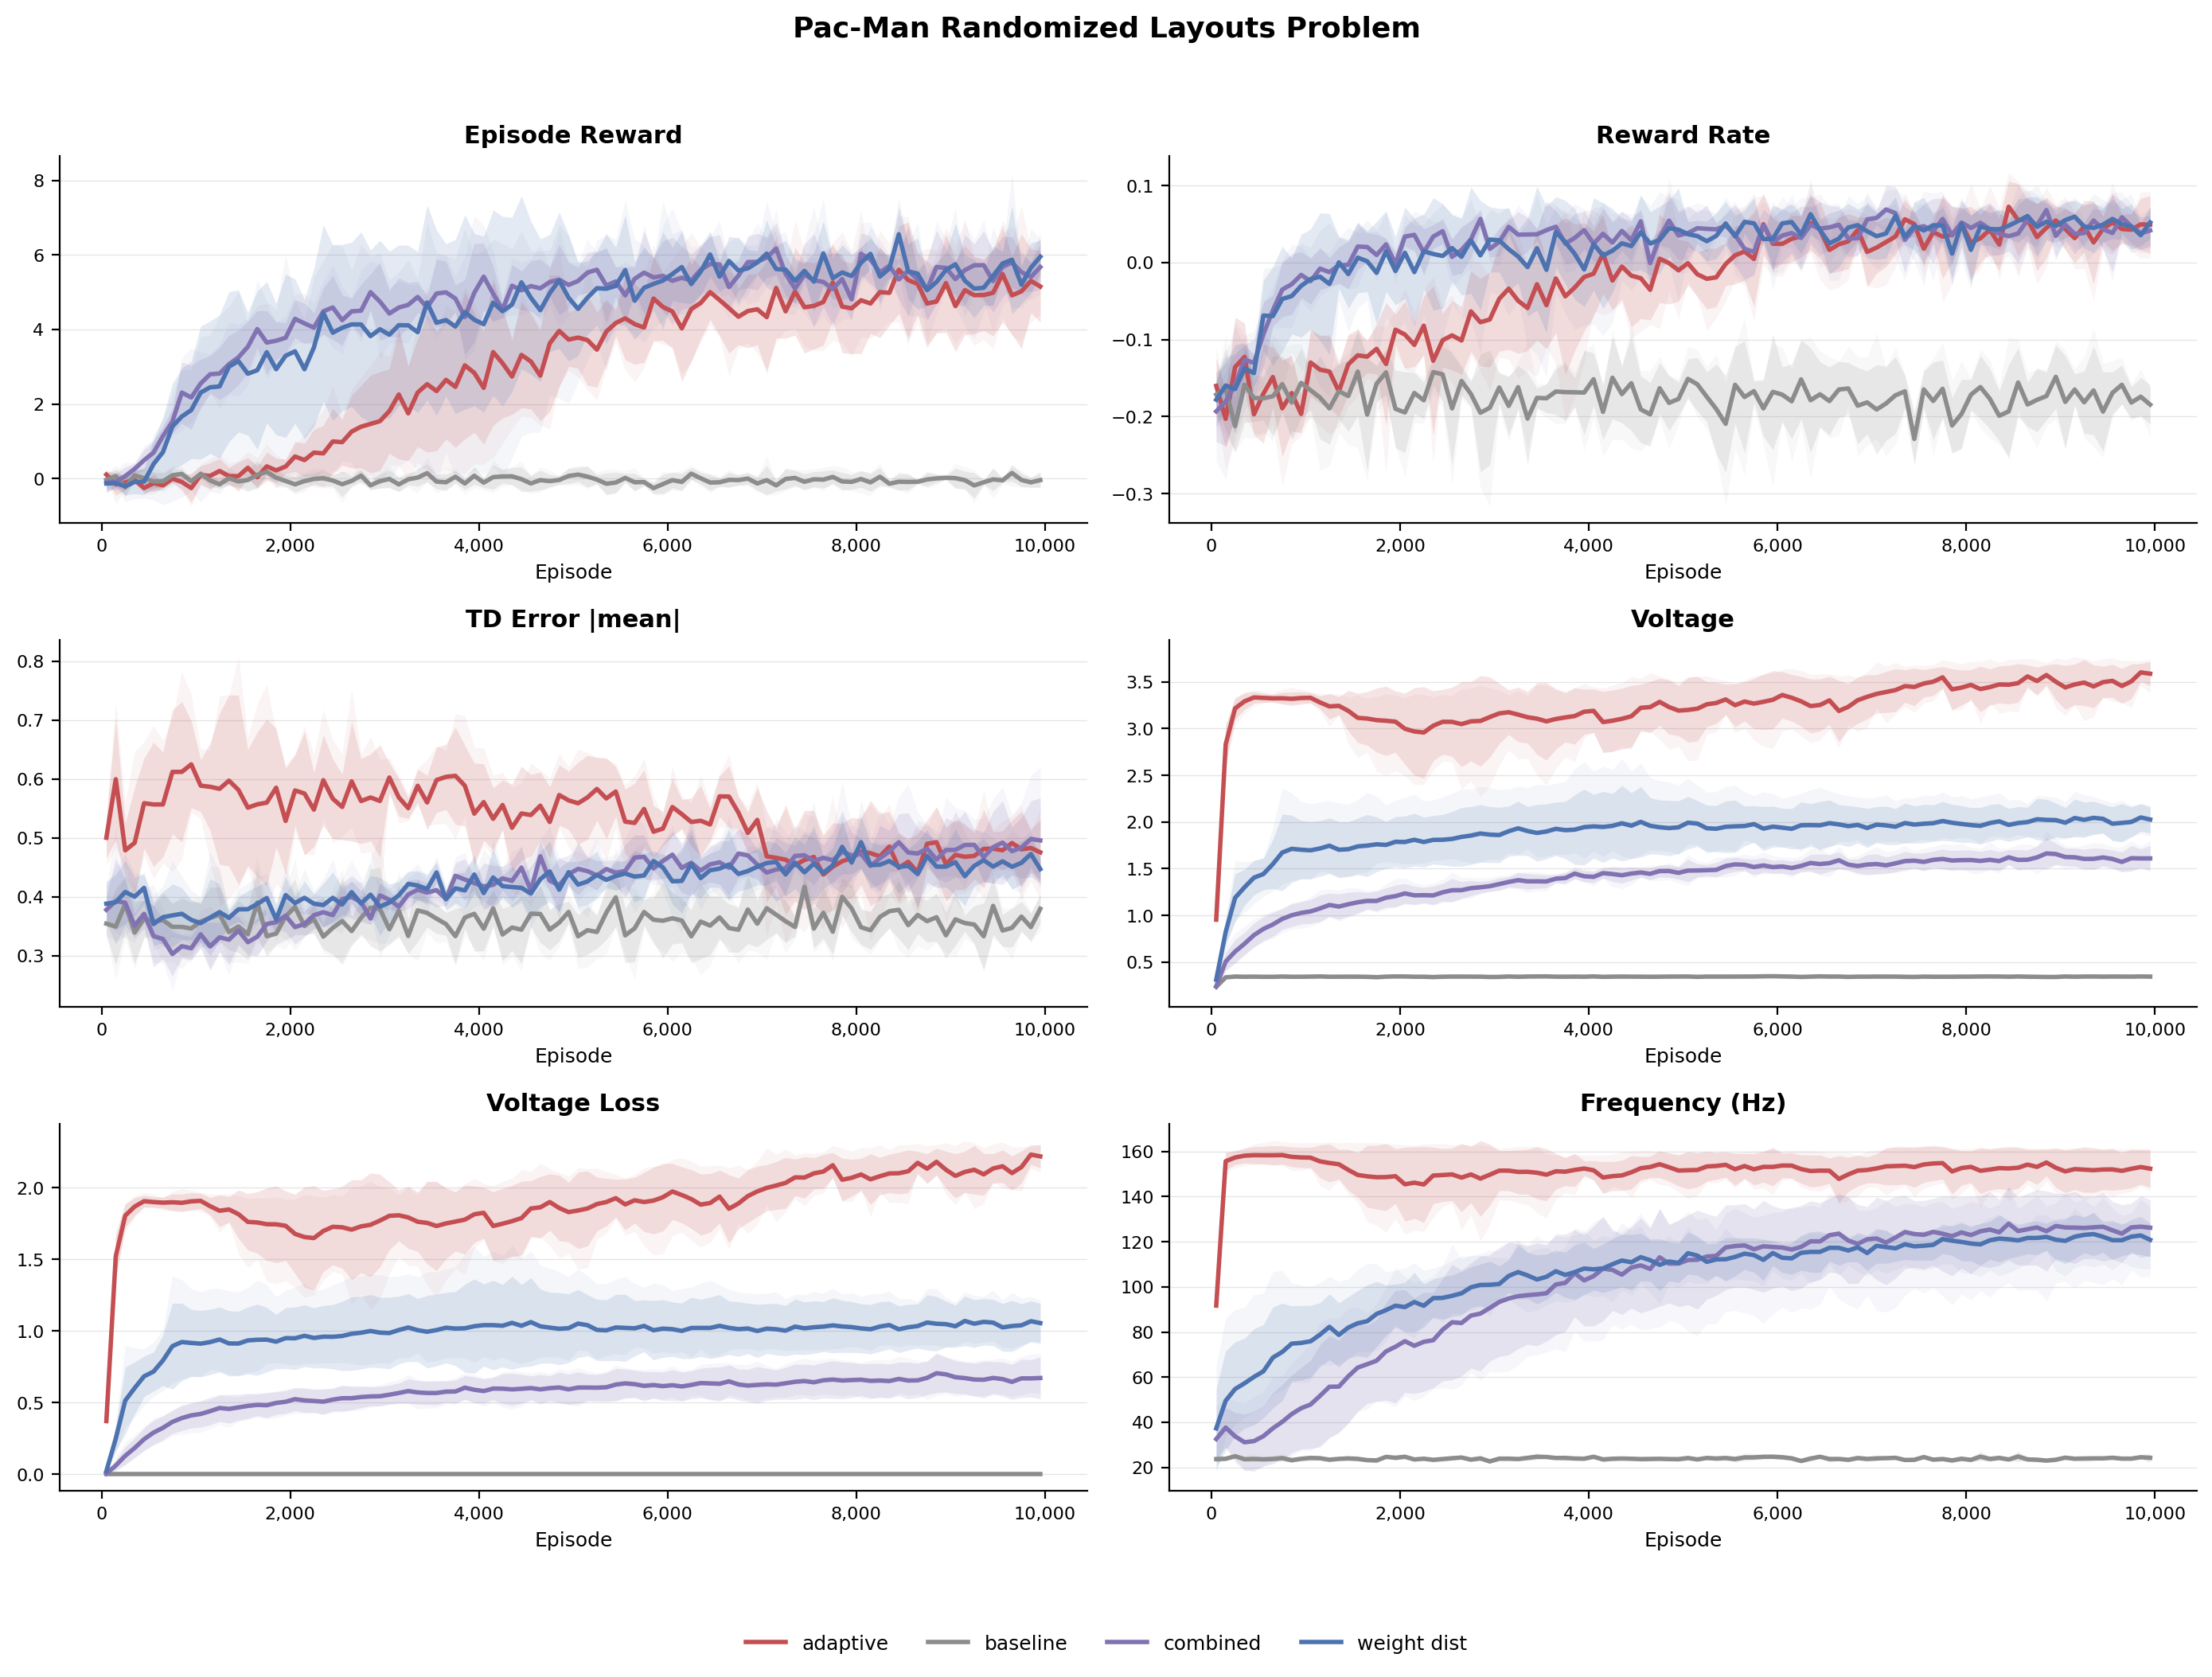
\includegraphics[width=\linewidth]{images/PacManComparison.png}
    \end{column}
  \end{columns}
\end{frame}

% ---- 5. HEADLINE: robustness to a broken neuron model --------
\begin{frame}{Robustness to a changed neuron model on Pac-Man}
  \begin{columns}[T]
    \begin{column}{0.4\textwidth}
      Disable membrane integration during the refractory period, a change to
      the standard ALIF dynamics.
      \vfill
      {\color{accent2}\aeprop} fails to learn at all;
      {\color{accent3}\deprop} keeps learning.
      \vfill
      \begin{alertblock}{Why}
        We don't have a clean mechanistic account of the asymmetry, only
        that \deprop{}'s perturbation-based credit is, empirically, far less
        sensitive to this change than \aeprop{}'s structured feedback, in this task.
      \end{alertblock}
    \end{column}
    \begin{column}{0.6\textwidth}
      \centering
      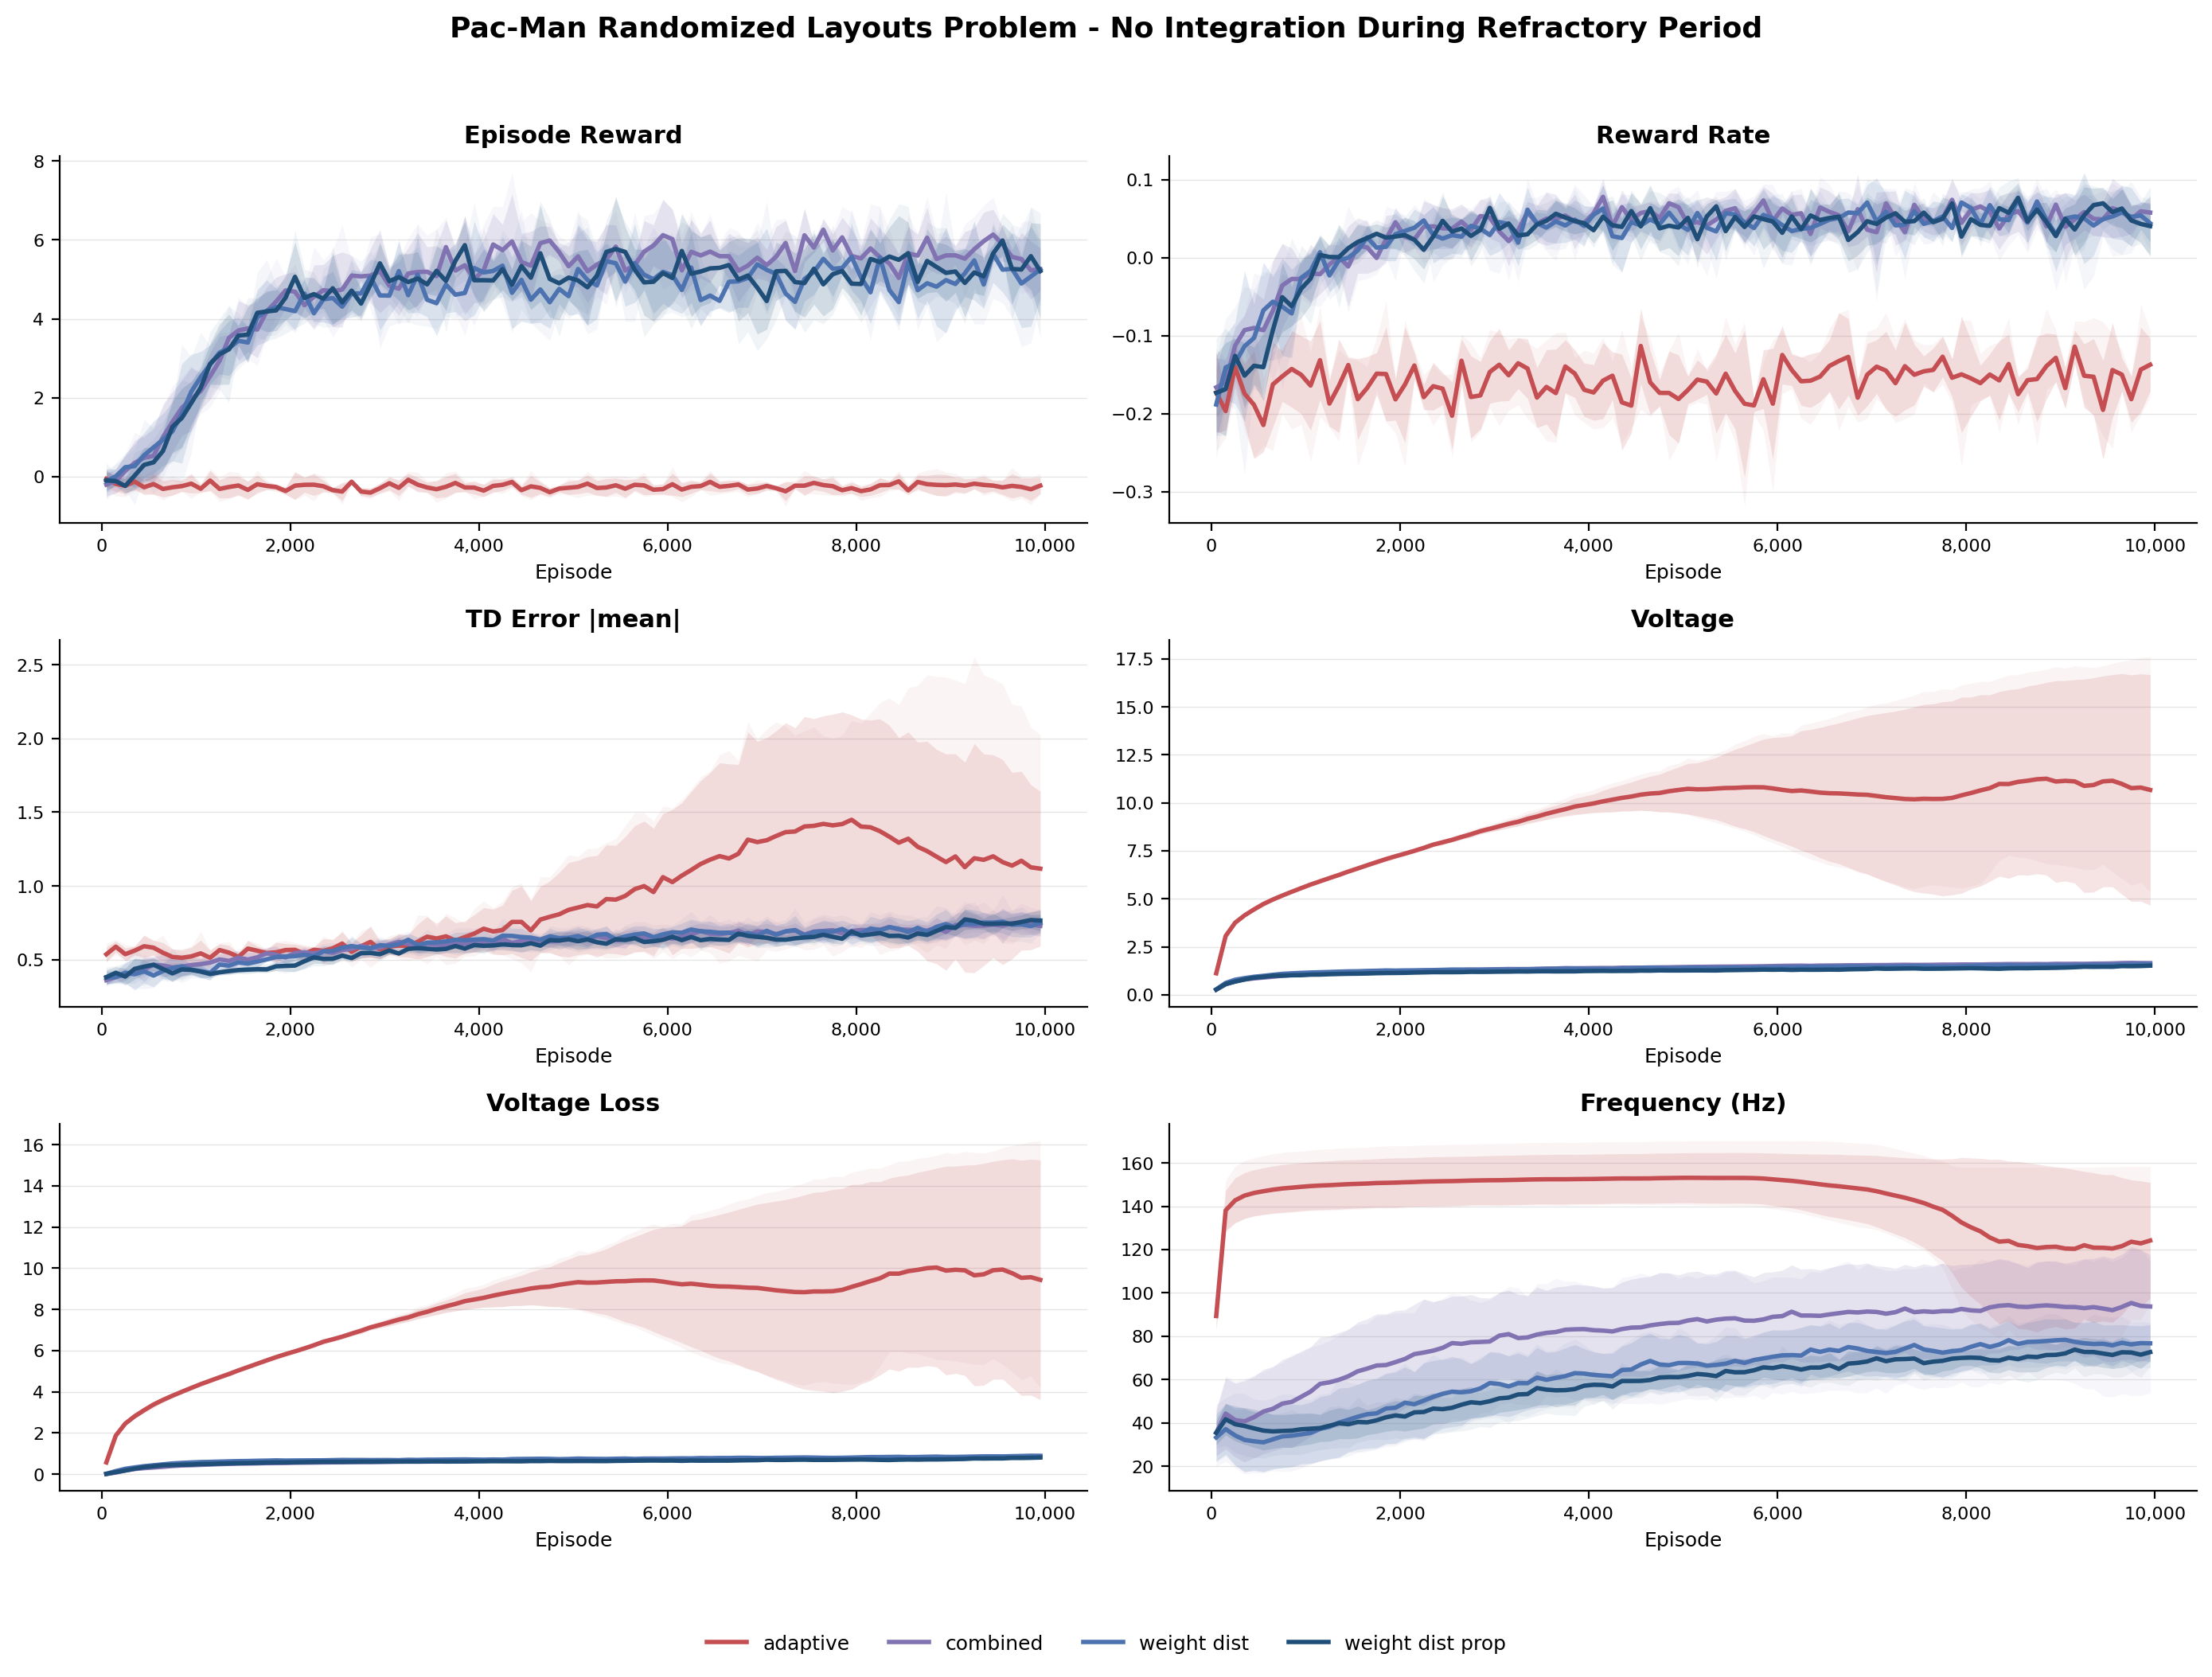
\includegraphics[width=\linewidth]{images/PacManComparisonNoIntegration.png}\\
    \end{column}
  \end{columns}
\end{frame}

\begin{frame}{Corroboration for value representation claim}
  \begin{columns}[T]
    \begin{column}{0.4\textwidth}
      The same value-representation advantage appears here: distributed e-prop's
      critic tracks the reward structure more cleanly, despite carrying no
      explicit value gradient in the recurrent update.
    \end{column}
    \begin{column}{0.6\textwidth}
      \centering
      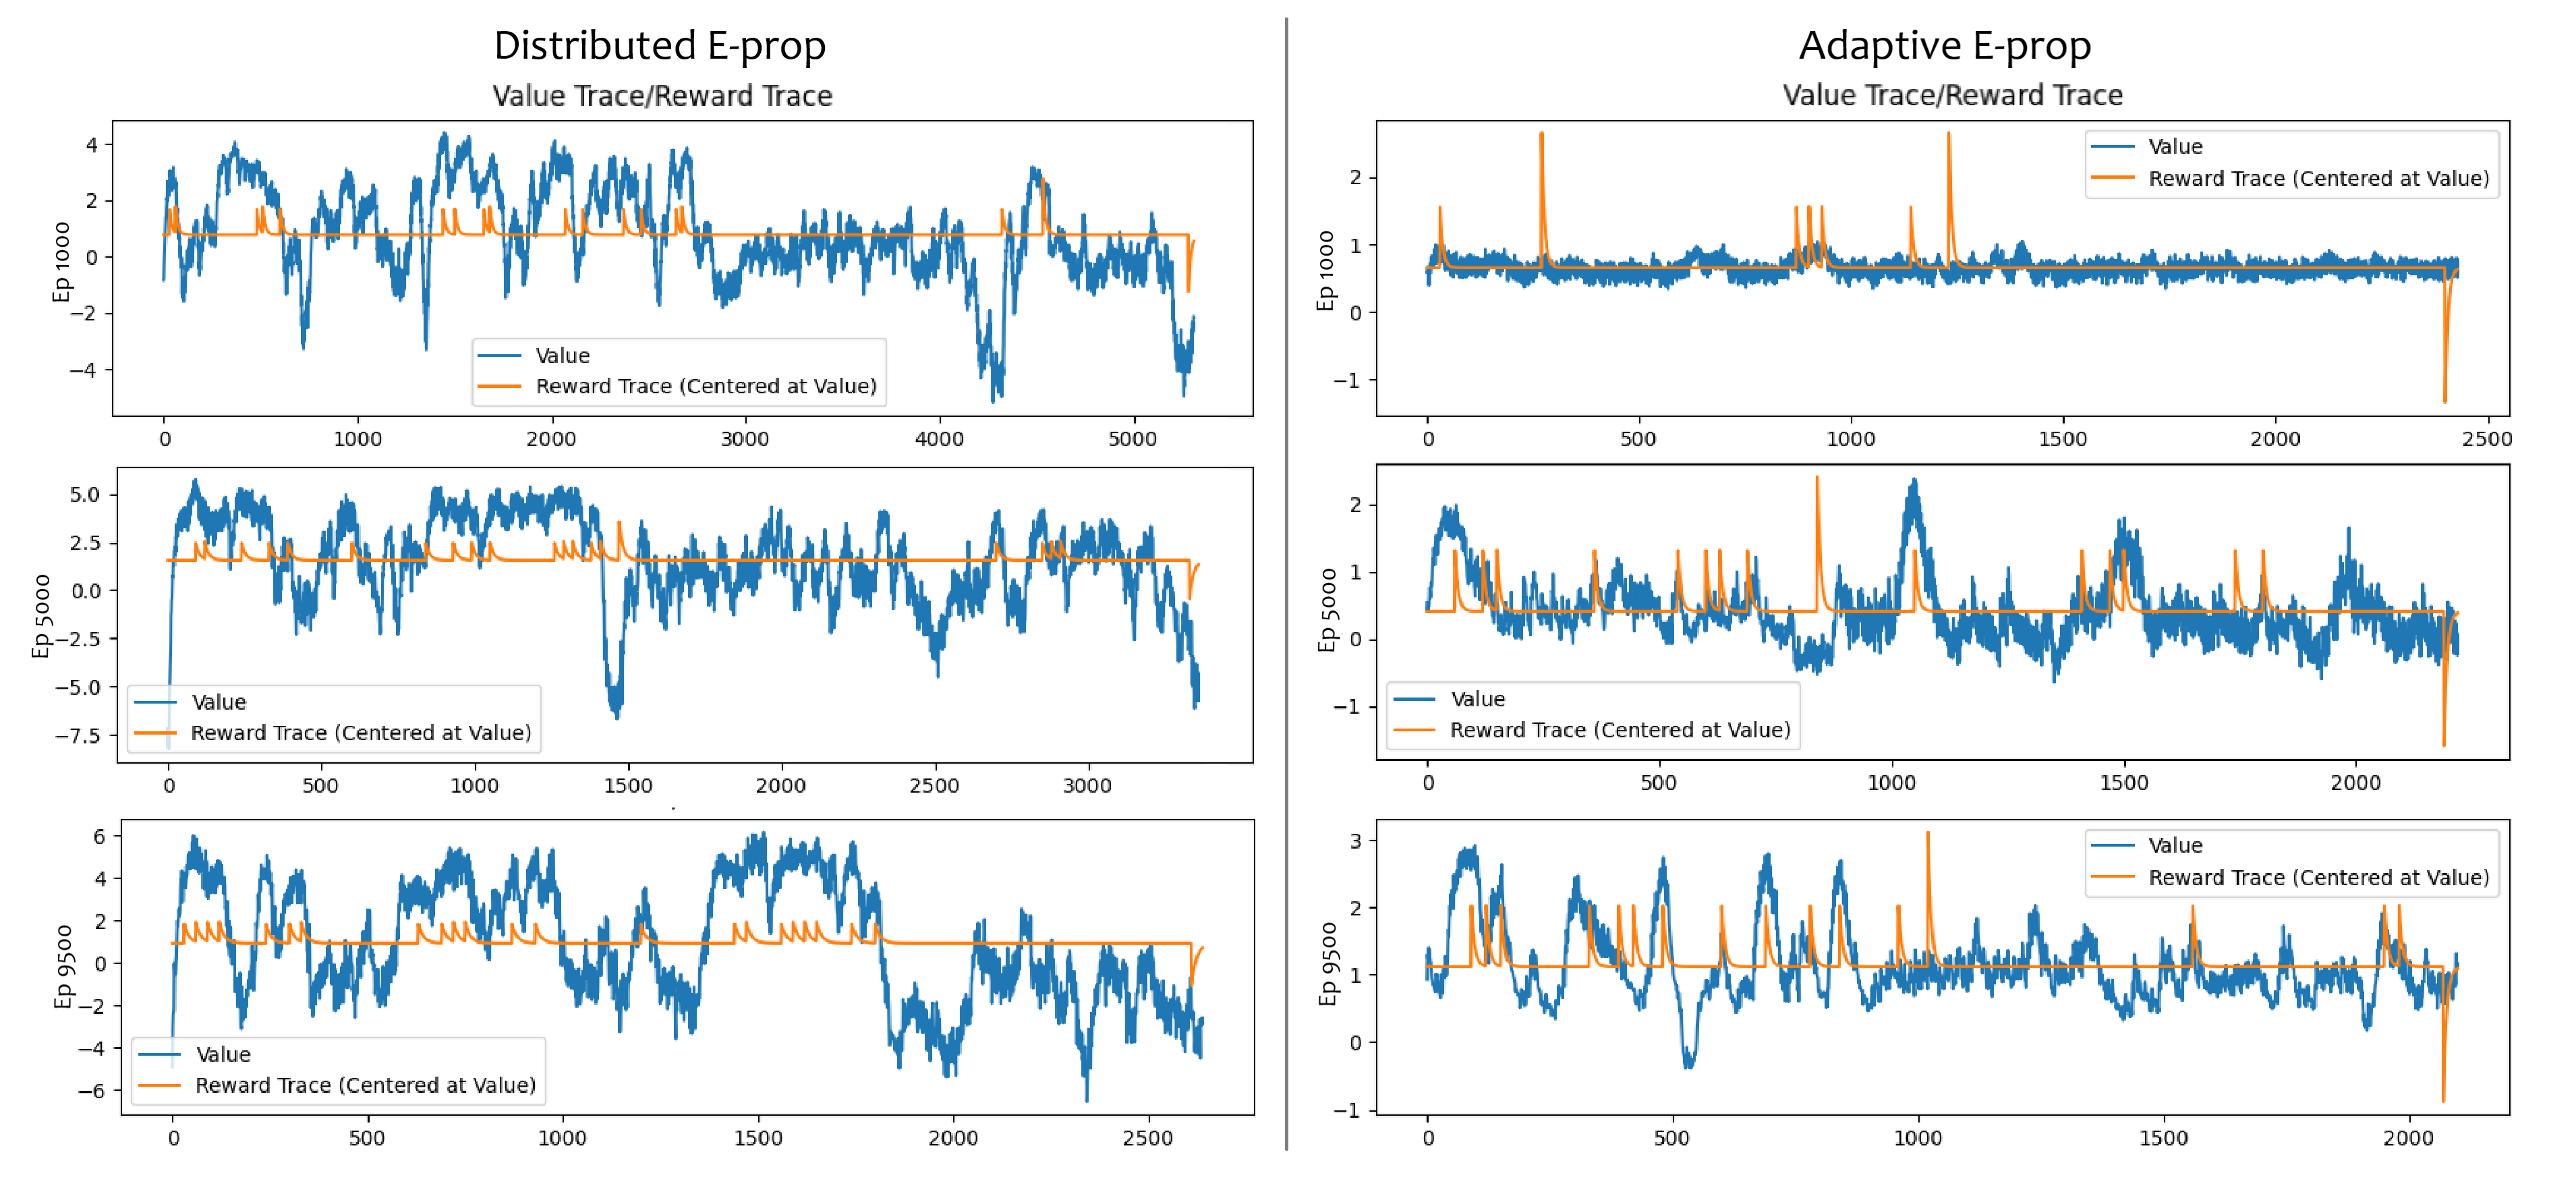
\includegraphics[width=\linewidth]{images/ValueFunctionPacManComparison.png}
    \end{column}
  \end{columns}
\end{frame}

% ---- 7. Nuance: lambda robustness reverses -------------------
\begin{frame}{Neither rule wins everywhere}
  \begin{columns}[T]
    \begin{column}{0.48\textwidth}
      \begin{block}{$\lambda$-robustness reverses}
        On \textbf{Snake}, adaptive seems more invariant to $\lambda$; on
        \textbf{Pac-Man} it reverses.
        Robustness is \emph{task-dependent}, not intrinsic.
      \end{block}
    \end{column}
    \begin{column}{0.48\textwidth}
      \begin{block}{Possible budget artifact}
        This could be due to a budget artifact, as we have seen, adaptive takes more time to learn, and can learn better configurations with time.
      \end{block}
    \end{column}
  \end{columns}
  \vfill
  \begin{columns}[T]
    \begin{column}{0.6\textwidth}
      \centering
      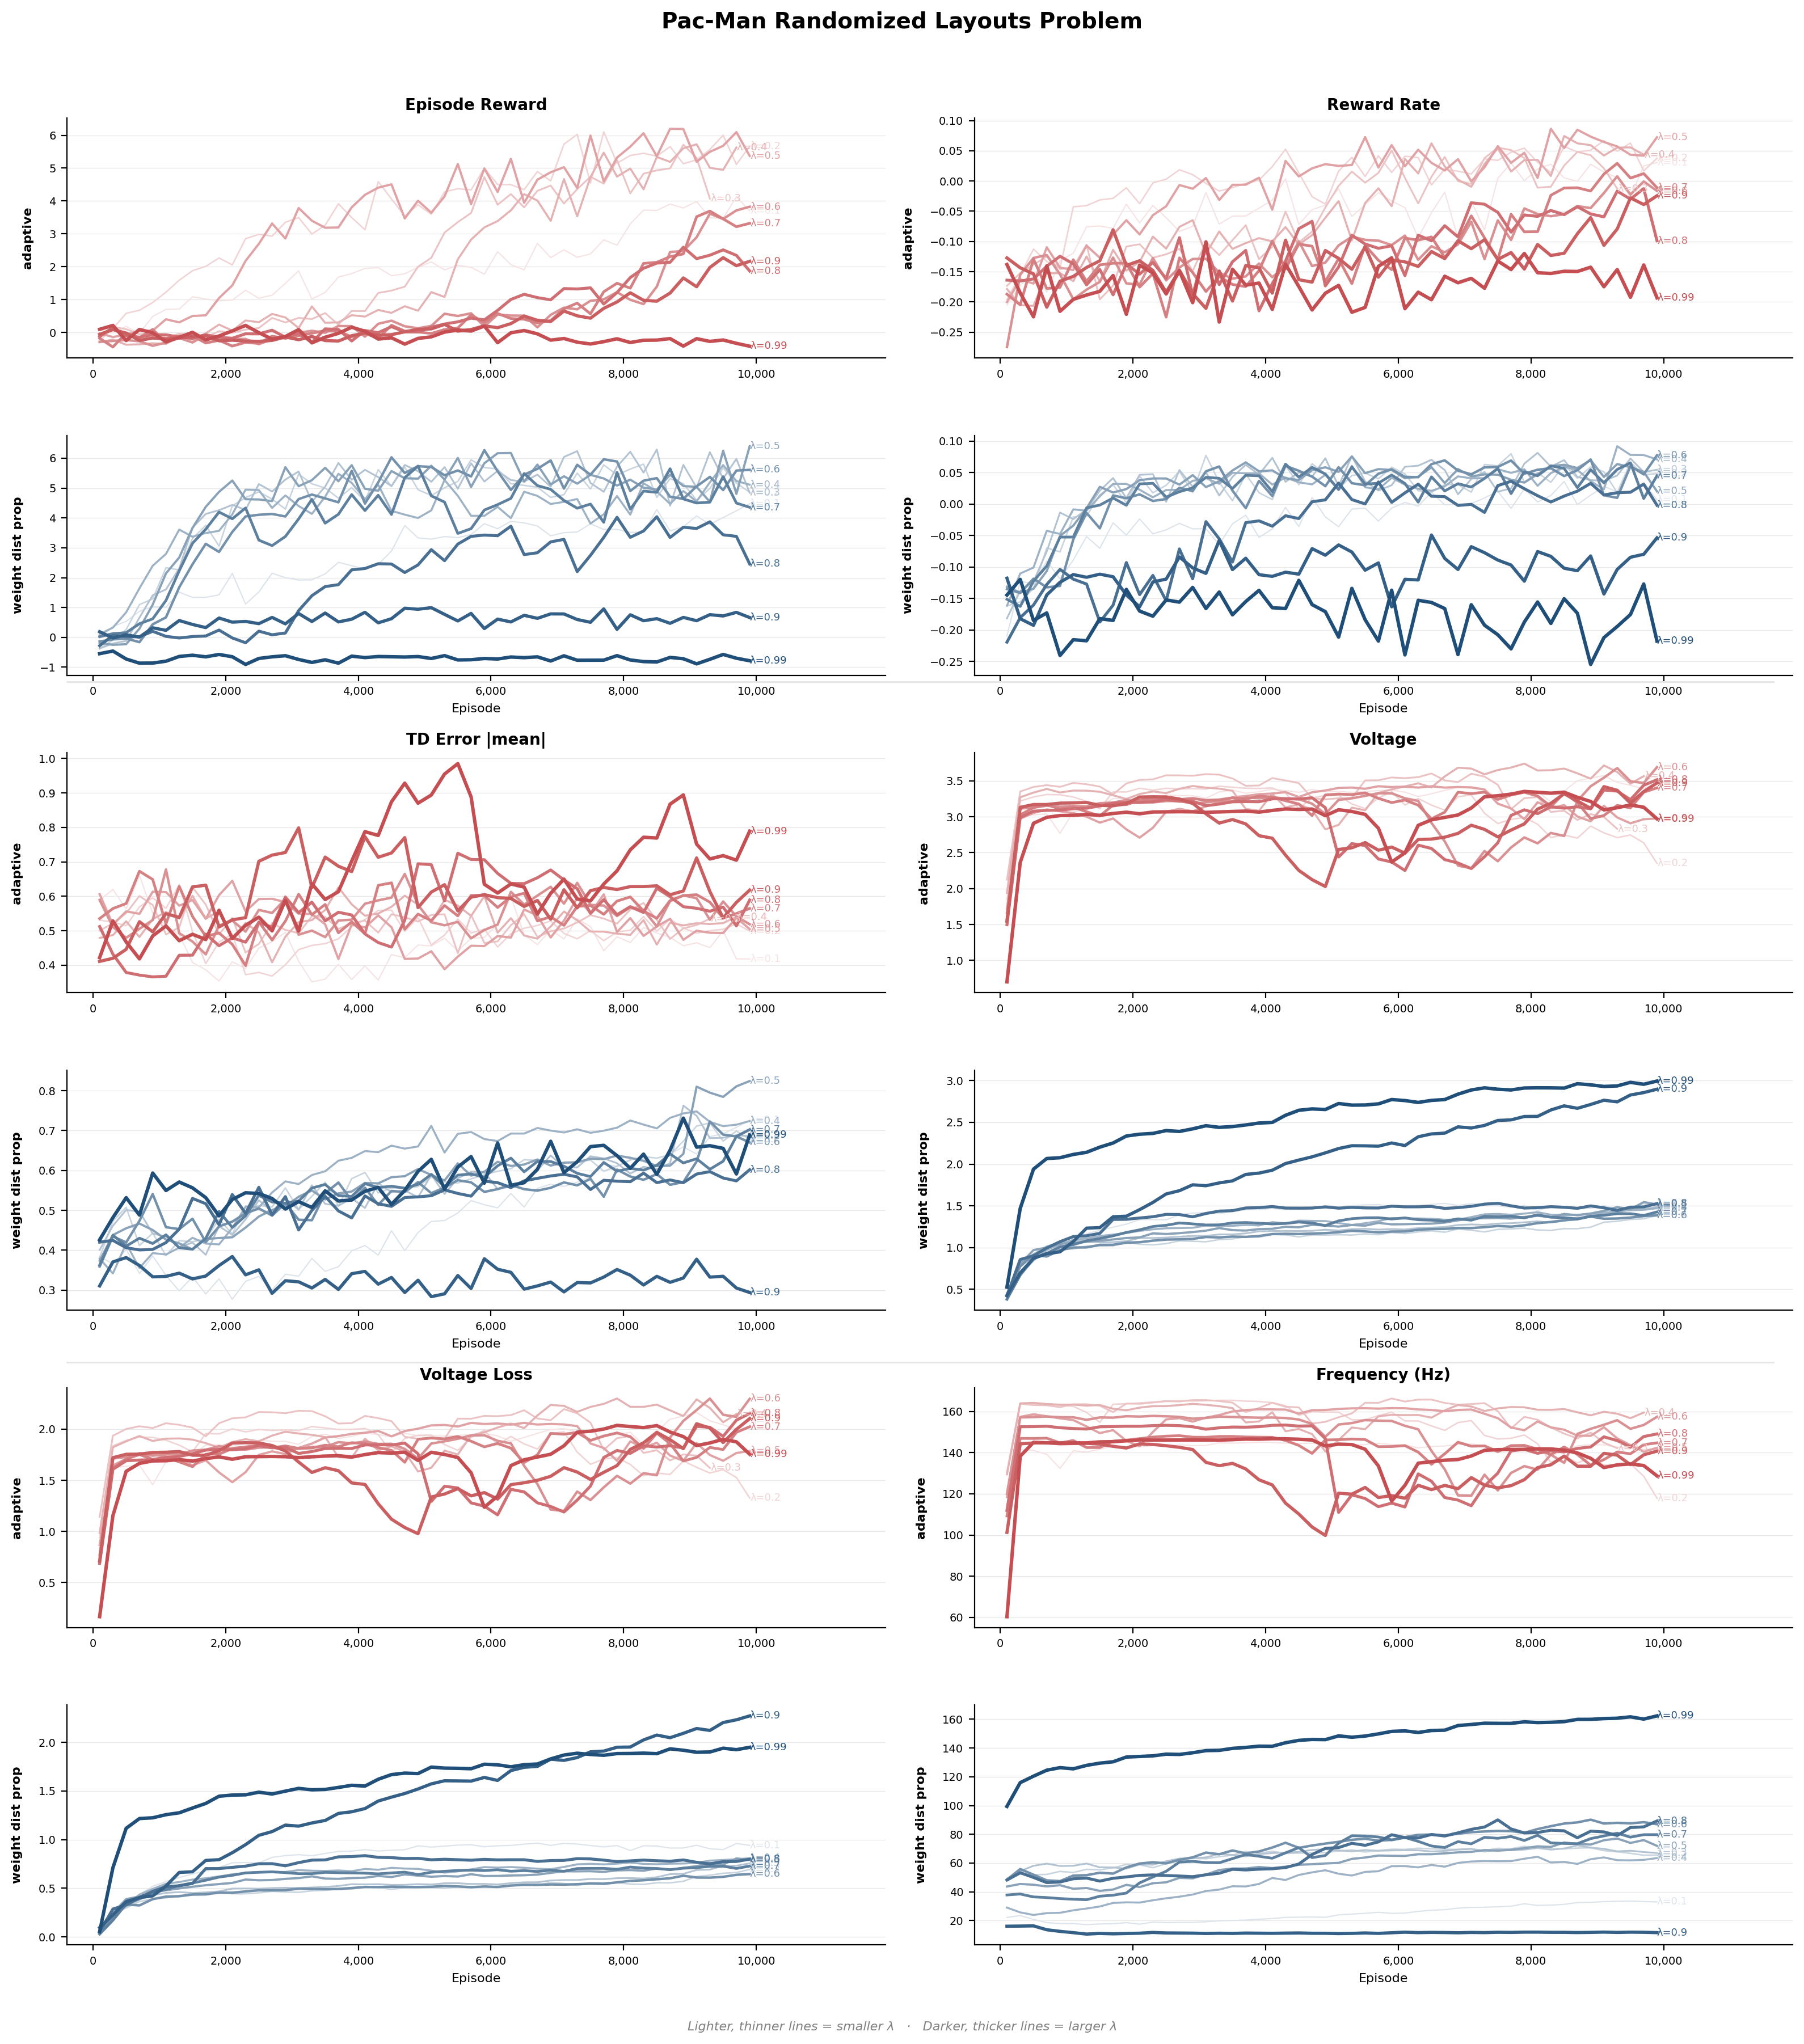
\includegraphics[width=\linewidth,clip,trim=0 29cm 0 0]{images/PacManComparisonLambdaGroups.png}
    \end{column}
  \end{columns}
\end{frame}

\begin{frame}{Neither rule wins everywhere}
  \begin{columns}[T]
    \begin{column}{0.4\textwidth}
      \begin{block}{Adaptive e-prop instability}
        As seen from previous results, adaptive e-prop seems to be more unstable during learning. With worse voltage results and in this case worse firing 
        rate results.
      \end{block}
      \begin{block}{Two failure modes}
        A poor $\lambda$ destabilizes distributed e-prop in opposite
        directions: runaway high firing, or excessive silence.
      \end{block}
    \end{column}
    \begin{column}{0.6\textwidth}
      \centering
      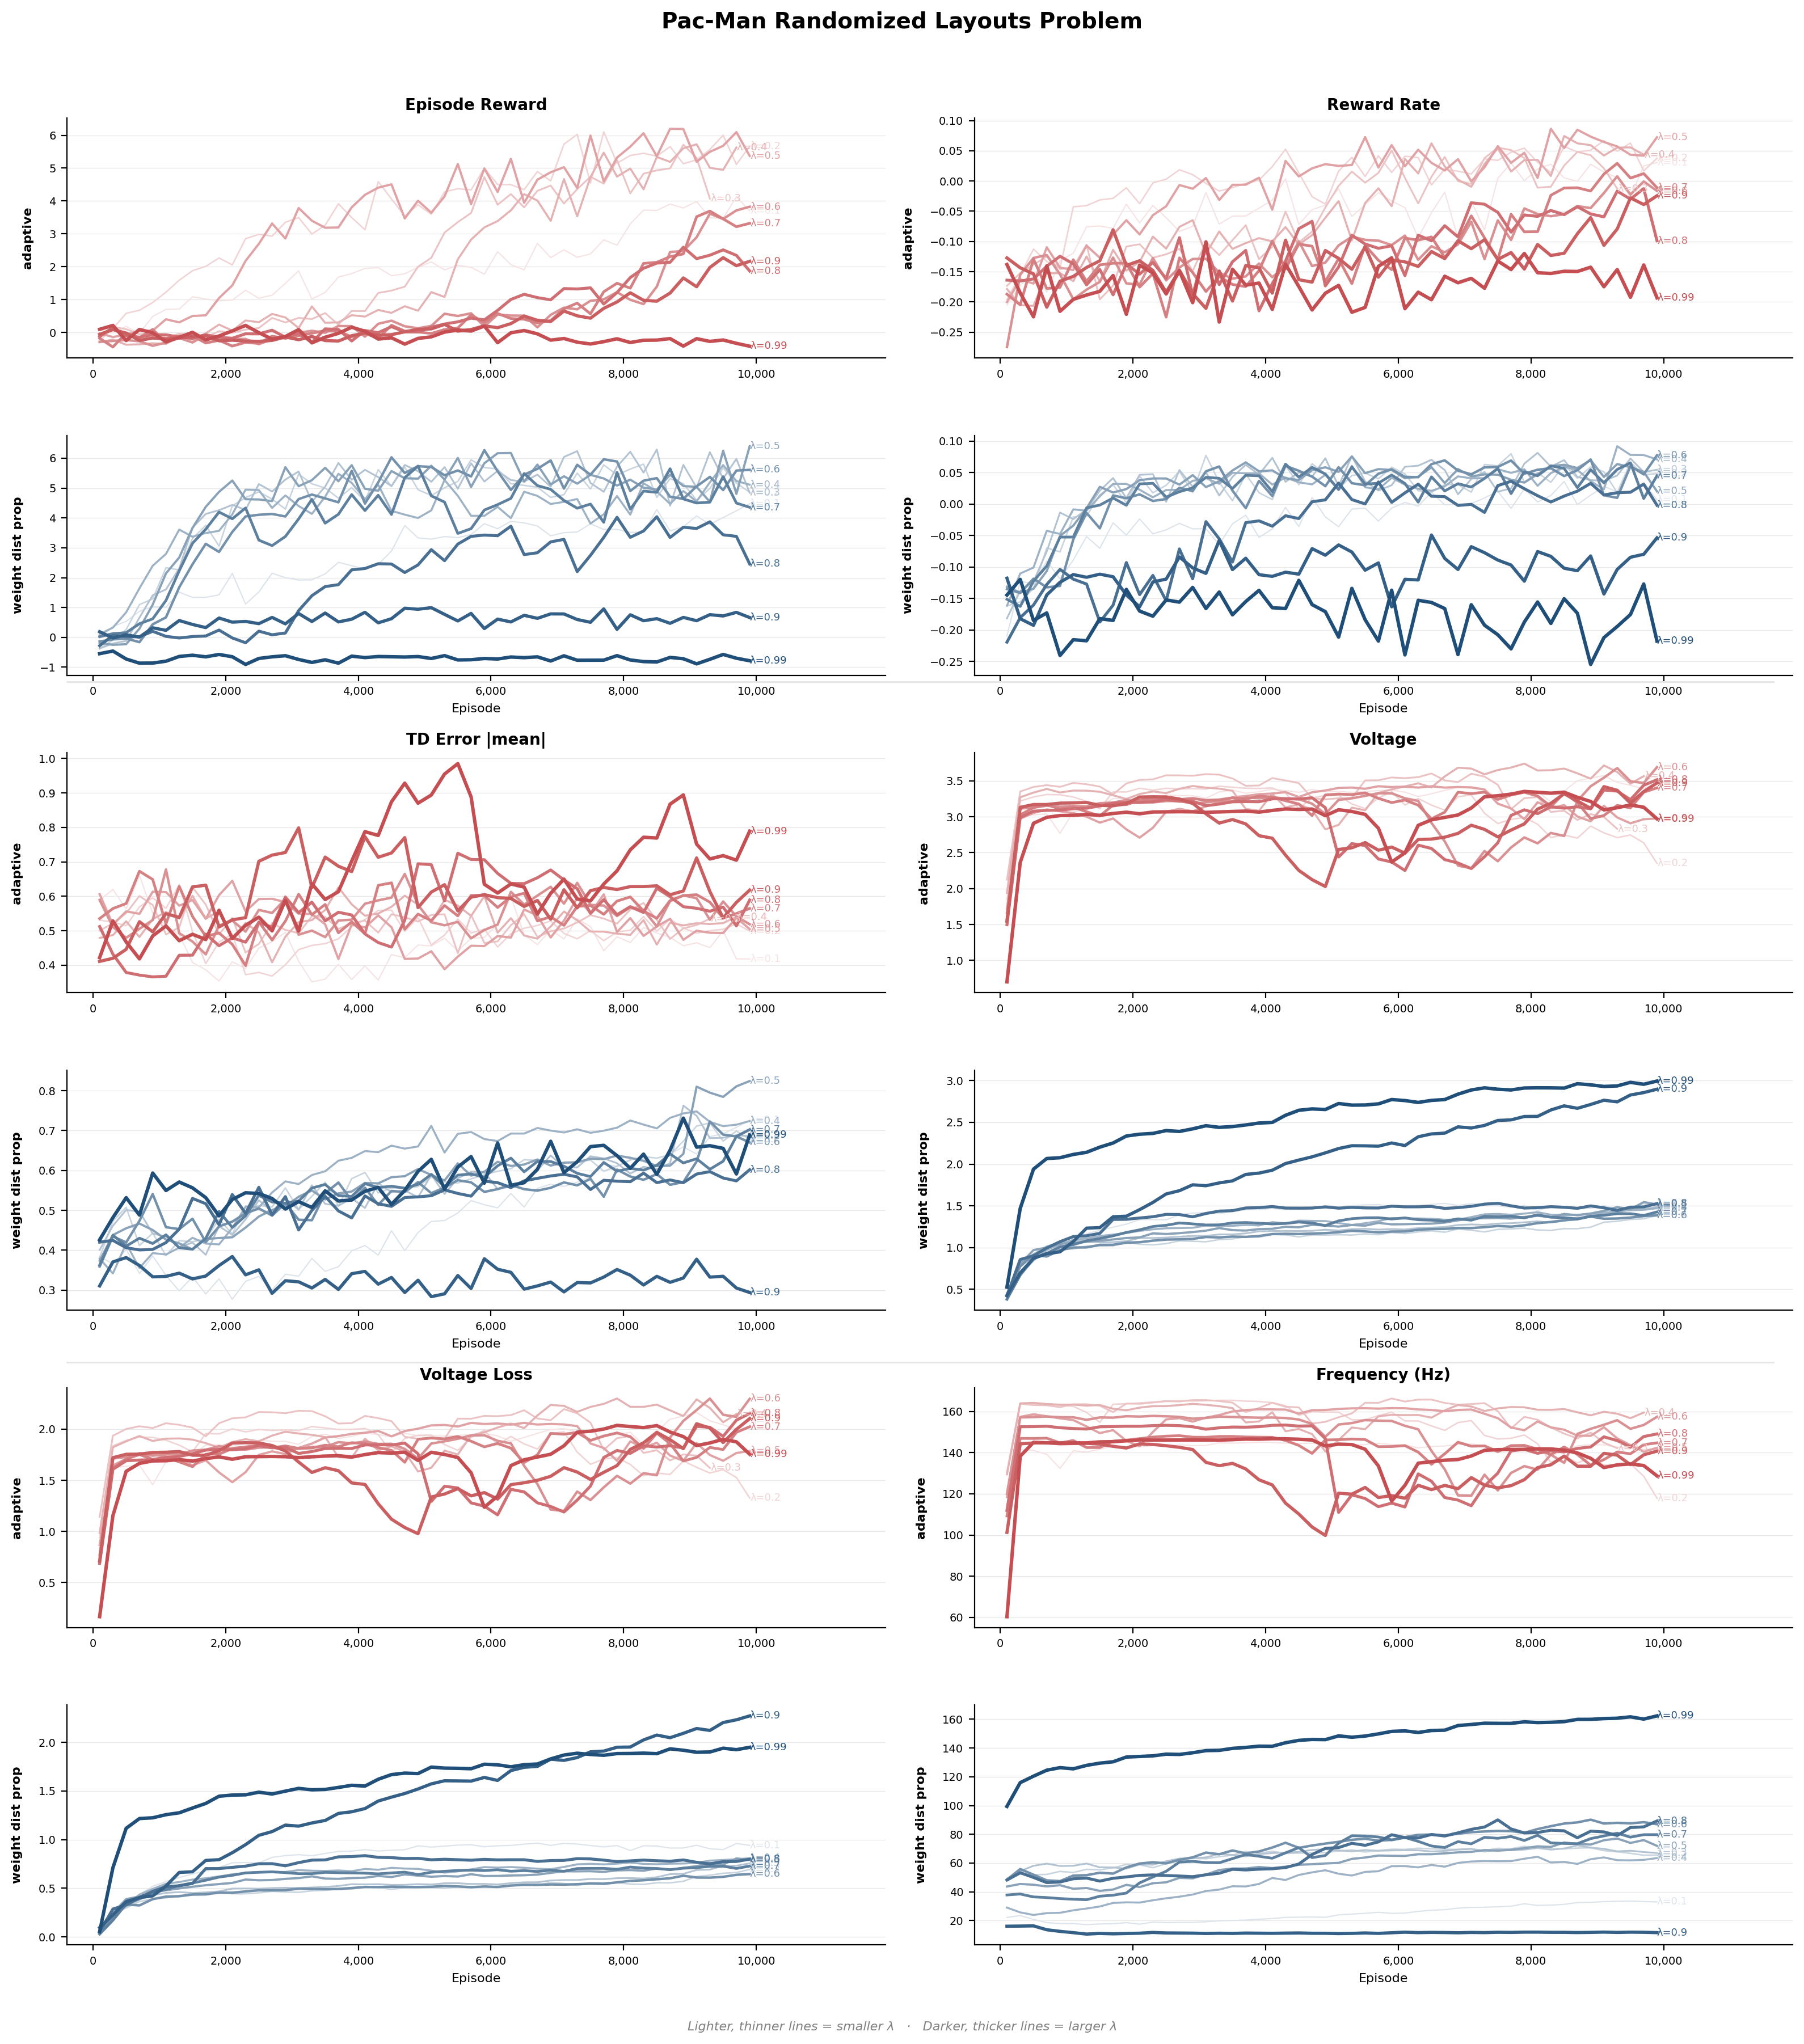
\includegraphics[width=\linewidth,clip,trim=0 0 0 16cm]{images/PacManComparisonLambdaGroups.png}
    \end{column}
  \end{columns}
\end{frame}

\begin{frame}{Best individual runs on Pac-Man}
  \scriptsize
  \setlength{\tabcolsep}{6pt}\renewcommand{\arraystretch}{1.1}
  \begin{tabular}{l r r r r}
    \toprule
    Run & Best100 RewardRate & Best100 Score & Wins\\
    \midrule
    weight dist (1)              & 0.1039 & \textbf{8.203} & 10 \\
    weight dist (3)              & 0.1106 & 8.144 & 9 \\
    weight dist (4)              & \textbf{0.1400} & 7.989 & 8 \\
    combined (NIDRP)(3)          & 0.1075 & 7.942 & 10 \\
    weight dist (2)              & 0.1050 & 7.827 & 4 \\
    adaptive (2)                 & 0.1214 & 7.809 & 6 \\
    adaptive (1)                 & 0.1195 & 7.753 & \textbf{14} \\
    weight dist prop $\lambda{=}0.3$ & 0.1173 & 7.649 & 8 \\
    combined (1)                 & 0.1090 & 7.614 & 7 \\
    adaptive $\lambda{=}0.5$     & 0.1228 & 7.603 & 3 \\
    combined (NIDRP)(2)          & 0.1046 & 7.482 & 5 \\
    combined (NIDRP)(5)          & 0.1081 & 7.476 & 10 \\
    \bottomrule
  \end{tabular}
  \vspace{0.5em}
  \footnotesize 
  
  Dominated by distributed variants (the two best by score belong to the
  \emph{weight dist} variant), though adaptive has the single highest-winning run.
  NIDRP $=$ no integration during refractory period. (Top 12 of 26.)
\end{frame}

\begin{frame}{The sparse-reward wall on Connect Four}
  \begin{columns}[T]
    \begin{column}{0.4\textwidth}
      A single terminal reward across a whole game, the hardest credit problem.
      \vfill
      \textbf{No rule reaches a positive reward} ($\sim$300k episodes).
      Variant \aeprop{} alone shows a slow upward trend, but, at the cost of steadily
      growing voltage and voltage loss. The \emph{baseline} stays
      inert.
    \end{column}
    \begin{column}{0.6\textwidth}
      \centering
      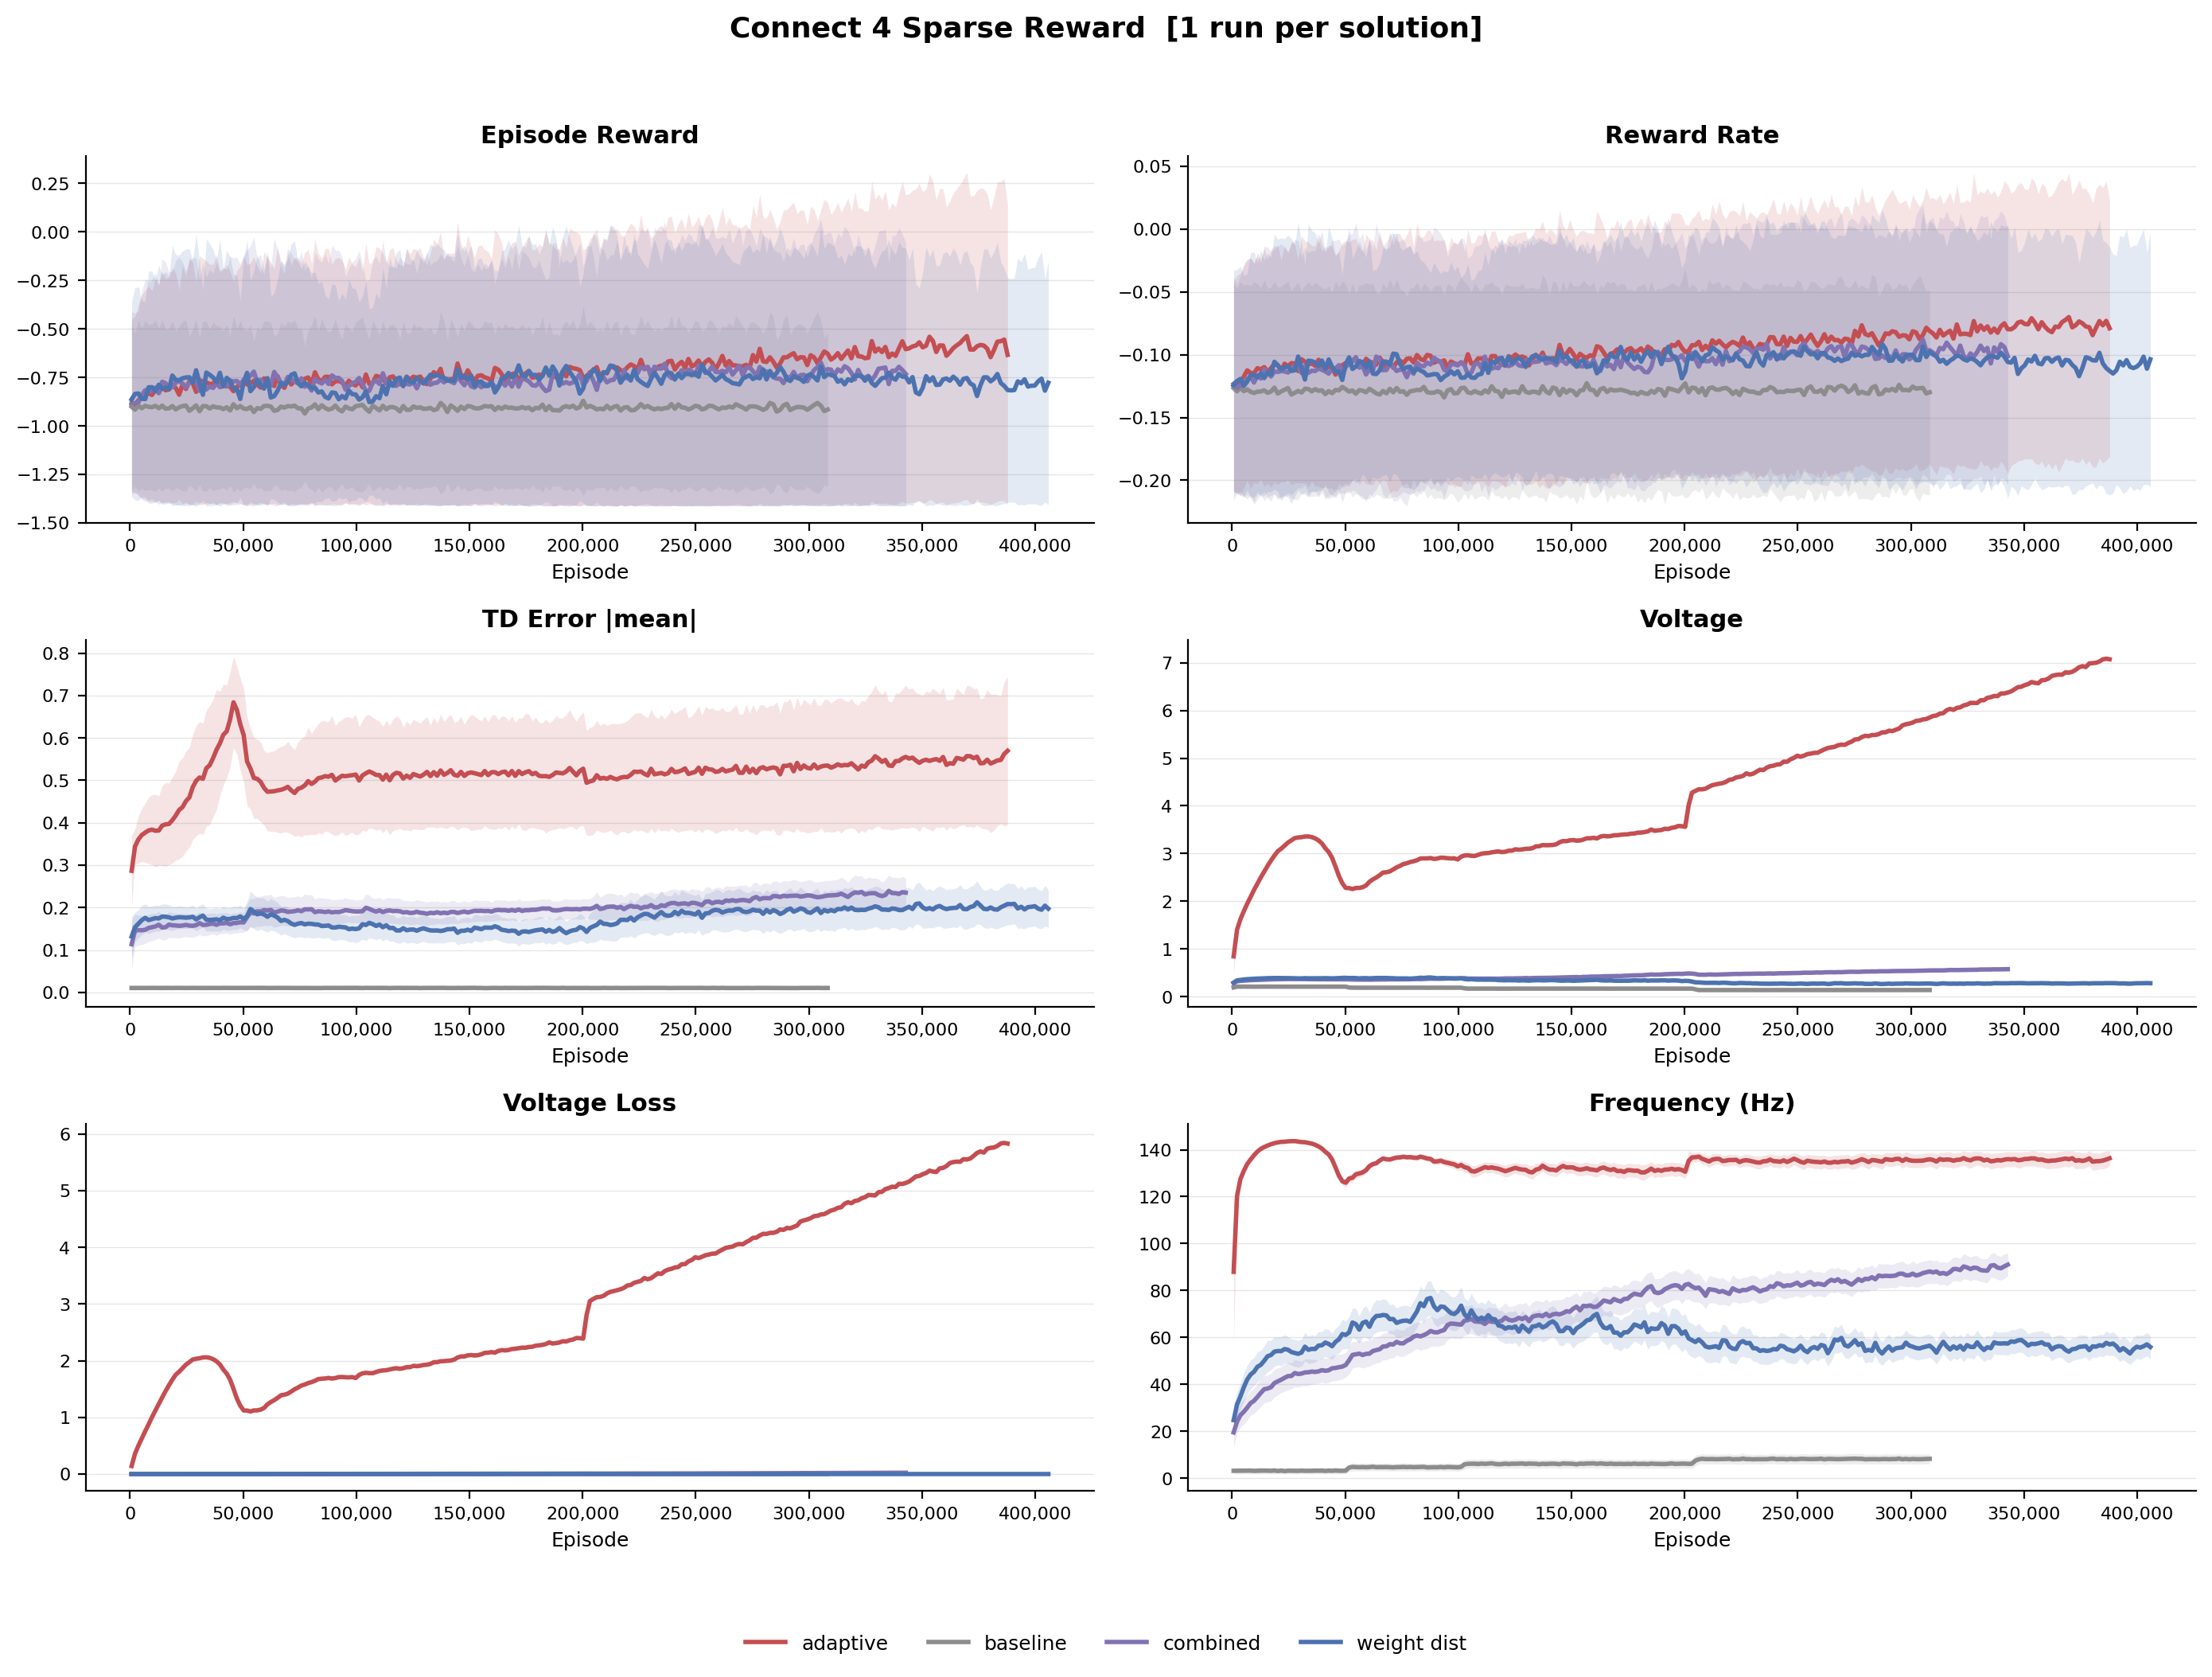
\includegraphics[width=\linewidth]{images/comparison_misc_1_runs.png}\\
    \end{column}
  \end{columns}
\end{frame}

% ============================================================
%  CHUNK 5 / 6 : Conclusions
% ============================================================
\section{Conclusions}

% ---- 1. What we found ---------------------------------------
\begin{frame}{What we found}
  \begin{columns}[T]
    \begin{column}{0.45\textwidth}
      \begin{block}{Competitive without feedback weights}
        Matches (sometimes outpaces) adaptive e-prop, despite discarding
        structured feedback entirely.
      \end{block}
      \begin{block}{Genuinely different mechanisms}
        Distinct dynamics on all experiments and depth/$\lambda$ sensitivities, not
        interchangeable variants of one rule, some hyperparameters work for one and not for the other on specific tasks.
      \end{block}
    \end{column}
    \begin{column}{0.45\textwidth}
      \begin{block}{Enables local reward shaping}
        A perturbation-gated voltage reward stabilizes dynamics, where the
        same term was found to make standard e-prop diverge.
      \end{block}
      \begin{block}{More robust to changes in the model}
        Keeps learning on a neuron model where standard e-prop fails.
      \end{block}
    \end{column}
  \end{columns}
\end{frame}

% ---- 8. Honest accounting: where it falls short --------------
\begin{frame}{Where the solutions fall short}
  \begin{enumerate}
    \item \textbf{A lower asymptotic ceiling.} Distributed variants converge
          fast, then plateau; adaptive, after a slow start, can climb past them
          over long ($\sim$100k-episode) runs.
    \item \textbf{Connect Four stays unsolved.} On the maximally sparse task,
          \emph{no} rule reached a usable policy, the adaptive variant shows the only
          positive trend.
    \item \textbf{Firing rates run high.} Across every rule and task, rates
          settle at $\approx 130$–$170$~Hz, far above the set target of
          $10Hz$. Rate regularization doesn't seem enough, or the formulation of the tasks demands these firing rates for effective learning on these architectures.
  \end{enumerate}
\end{frame}

% ---- 2. The answer ------------------------------------------
\begin{frame}{The answer}
  \begin{block}{}
    \centering\large
    A single, globally broadcast scalar \emph{is enough} to train recurrent
    spiking networks effectively, online and with constant memory.
  \end{block}
  \vfill
  \begin{alertblock}{\ldots with qualifications}
    \begin{itemize}
      \item A lower asymptotic ceiling in some settings.
      \item The usable $\lambda$ range is task-dependent.
      \item The hardest, maximally sparse task (Connect Four) is still out of
            reach.
    \end{itemize}
  \end{alertblock}
\end{frame}

% ---- 3a. Limitations ----------------------------------------
\begin{frame}{Limitations}
  \begin{itemize}
    \item A lot of experiments are single run experiments, which limits the possible           claims they can verify.
    \item No TBPTT upper-bound baseline. The online, constant-memory
          setting rules it out, so the ceiling for the architectures used is unknown.
    \item Several proposed extensions of the rule didn't work reliably enough to
          include in the main results.
    \item $\gamma$ was fixed to $0.5$ from initial exploration, its role is
          left largely uncharted (see future work).
  \end{itemize}
\end{frame}

% ---- 3b. Future work - research directions (full slide) -----
\begin{frame}{Future work}
  \small
  Beyond further sweeps, the open questions cluster around letting the network
  \emph{shape its own learning}:
  \vspace{0.4em}
  \begin{columns}[T]
    \begin{column}{0.5\textwidth}
      \begin{itemize}\setlength\itemsep{0.5em}
        \item \textbf{Self-trained learning signals.} An online-trained learning signal, online meta-learning
        ~\citep{OneShotEprop}.
        \item \textbf{Self-modulated, state-dependent exploration.} Make
              $\sigma_j$ depend on context (e.g.\ value uncertainty), a learned controller over the network's exploration, and therefore learning.
        \item \textbf{A broader family of local reward signals.} Beyond voltage
              and firing rate: spike sparsity, neighbour correlations,
              informativeness - many local rewards alongside the global task
              reward.
      \end{itemize}
    \end{column}
    \begin{column}{0.5\textwidth}
      \begin{itemize}\setlength\itemsep{0.5em}
        \item \textbf{Structural plasticity \& online rewiring.} Adapt the
              \emph{topology} itself, not just weights - potentially taming the
              pervasive high-firing regime.
        \item \textbf{Deliberate fusion of feedback signals.} Combine structured
              and perturbation-based credit dynamically (e.g.\ weight by their
              agreement), rather than a plain sum.
        \item \textbf{Tasks demanding long-term memory.} Horizons of hundreds–
              thousands of steps to stress the $\lambda$ credit window and the
              adaptive-threshold timescale.
      \end{itemize}
    \end{column}
  \end{columns}
\end{frame}

% ---- 4. Closing --------------------------------------------
\begin{frame}[plain]
  \centering
  {\color{accent}\Large\textbf{Thank you}}\\[1ex]
  Questions welcome.\\[2ex]
  \small
  Edgar Sarria Tenes\\
  Supervisor - Enrique Romero Merino\\
  FIB · UPC - BarcelonaTech
\end{frame}

% ============================================================
%  References
% ============================================================
\begin{frame}[allowframebreaks]{References}
  \bibliographystyle{plainnat}
  \bibliography{references}
\end{frame}

% (chunks 2–6 go here, before \end{document})

\end{document}